% This is the body of your document. You may copy-paste it into your main document
% (dissertation.tex, masterreport.tex, masterthesis.tex, treatise.tex), or edit it here.


% \copyrightpage  % Produces the copyright page. Optional.

% \commcertpage   % Produces the Committee Certification
			%   of Approved Version page (doctoral)
			%   or Signature page (masters).
			%		20 Mar 2002	cwm
                % Required.


\titlepage      % Produces the title page. Required.


%%%%%%%%%%%%%%%%%%%%%%%%%%%%%%%%%%%%%%%%%%%%%%%%%%%%%%%%%%%%%%%%%%%%%%
% Dedication and/or epigraph are optional, but must occur here.      %
%%%%%%%%%%%%%%%%%%%%%%%%%%%%%%%%%%%%%%%%%%%%%%%%%%%%%%%%%%%%%%%%%%%%%%
% \begin{dedication}		% Optional
% To all future Longhorn graduate students.
% \end{dedication}

% \begin{epigraph}		% Optional
% \begin{center}
%     \textit{What starts here changes the world.}
%     \\\hspace{4em}---University of Texas at Austin
% \end{center}
% \end{epigraph}

%%%%%%%%%%%%%%%%%%%%%%%%%%%%%%%%%%%%%%%%%%%%%%%%%%%%%%%%%%%%%%%%%%%%%%
% Acknowledgements and/or preface are optional, but must occur here. %
%%%%%%%%%%%%%%%%%%%%%%%%%%%%%%%%%%%%%%%%%%%%%%%%%%%%%%%%%%%%%%%%%%%%%%
\begin{acknowledgments}		% Optional
I would like to express my gratitude to all of the numerous people who have shaped my undergraduate experience into such a remarkable journey.

Foremost, I would like to thank Prof. Deepa Thomas, my advisor, for guiding me wonderfully through my research over the last two years. I am grateful for all her insights as we studied the hundreds of plots I made, for her interest in all the things I tried, and for the many opportunities she has created for me to present my project,
% from small updates at group meetings to presentations for the ePIC Collaboration, 
which has shown me how rewarding it can be to carry on a multi-stage project and to share my work with others.

I would like to thank Dr. Shyam Kumar, Dr. Rongrong Ma, and others in the ePIC Collaboration for lending me the data samples, analysis codes, and research expertise necessary to complete this project. I would also like to thank everyone in the UT Relativistic Heavy Ion Group for providing me with such a supportive space to learn and grow.

Beyond this project, I have also been so fortunate to receive the support of many peers and mentors across biology, chemistry, and physics. I would like to thank them all---the Microbe Hackers group, the Sessler group, my REU cohort at Notre Dame, the JAM Collaboration, my fellow interns at Jefferson Lab, among others---for extending a hand to me and inspiring my passion for research. I am also grateful to my fellow members of Texas Wushu, past and present, and my friends from Katy for keeping me in touch with life outside of academics.

Finally, I would like to thank my family---especially my mom and grandma who have always made sure I was warm, fed, and grounded, and my brother who has kept me company in Austin---for being my constant source of care and comfort throughout this nonlinear journey.

% Thank you all for this remarkable experience!


\end{acknowledgments}

% \begin{preface}		% Optional
% Readers, this document represents a great deal of time and effort. Enjoy. Cheers, \theauthor.
% \end{preface}

% The abstract is required. Note the use of ``utabstract'' instead of
% ``abstract''! This was necessary to fix a page numbering problem.
% The abstract heading is generated automatically.
% Do NOT use \begin{abstract} ... \end{abstract}.
%
\utabstract
The Electron-Ion Collider (EIC) will further our understanding of the quarks and gluons which constitute visible matter by imaging the internal structure of protons and nuclei with greater precision than ever achieved. High-energy collisions at the EIC will lead to the production of heavy flavor particles such as $D^0$-mesons, which serve as probes to the gluon distributions within the colliding protons and neutrons. In order to develop efficient methods of analyzing these $D^0$-mesons, we explore the application of boosted decision trees (BDTs), a type of machine learning model, to separate $D^0$ signals from background based on features of the $D^0\rightarrow\pi+K$ decay topology. We present a preliminary analysis in which we apply an existing BDT framework to new simulated data, which demonstrates the negative impacts of machine-background effects on the $D^0$ analysis. We then optimize the BDT framework by limiting the kinematic range of the data, selecting more effective topological features, and tuning the hyperparameters which govern the BDT model structure. Finally, we demonstrate the advantage of BDT based analysis over the topological cuts determined through non-machine learning methods.    % this includes the text from `abstract.tex`

\tableofcontents   % Table of Contents will be automatically
                   % generated and placed here. Required.

\listoftables      % Optional.
\listoffigures     % Optional.
% \listofillustrations     % Optional.
% \listofmaps      % Optional.
% \listofslides    % Optional.


%%%%%%%%%%%%%%%%%%%%%%%%%%%%%%%%%%%%%%%%%%%%%%%%%%%%%%%%%%%%%%%%%%%%%%
% Actual text starts here.					     %
%%%%%%%%%%%%%%%%%%%%%%%%%%%%%%%%%%%%%%%%%%%%%%%%%%%%%%%%%%%%%%%%%%%%%%
%
% Including external files for each chapter makes this document simpler,
% makes each chapter simpler, and allows for generating test documents
% with as few as zero chapters (by commenting out the include statements).
% Can even change the chapter order by merely interchanging the order
% of the include statements (something past contributors found helpful in their own
% dissertations =) ).
%

% \chapter{Introduction}
\section{Nuclear physics: understanding the fundamental constituents of matter}
All ordinary matter is made of atoms. Named after the Greek word {\it atomos}, meaning ``indivisible," atoms were once thought to be the most basic building blocks of nature. Today, we know that atoms are composite structures built from electrons, protons, and neutrons. Furthermore, protons and neutrons, collectively called ``nucleons," are themselves composed of quarks and gluons. The electron, quarks, and gluons are examples of elementary particles, the truly irreducible {\it atomos} of the universe. They are members of the Standard Model of particle physics, which is currently the best physical theory capable of describing three of the four fundamental forces: electromagnetism, the strong force, and the weak force. (The fourth force, gravity, is described by the theory of general relativity.) 

Although the existence of quarks and gluons has been experimentally verified, many aspects of their behavior remain elusive. How are the quarks and gluons distributed inside of protons and neutrons? How do these extremely light particles generate nearly all the mass in the visible universe? How do their interactions give rise to both ordinary and exotic forms of matter, from everyday nucleons and nuclei to the primordial quark-gluon plasma (QGP) that existed in the early universe? These are examples of the fundamental questions we study in high-energy nuclear physics.

At the frontier of these pursuits today is the Electron-Ion Collider (EIC). Currently being built at Brookhaven National Lab on Long Island, the EIC will allow us to probe the quarks and gluons within nucleons with greater precision than previously possible. To support these future experiments, in this thesis we explore the application of machine learning towards the development of efficient data analysis for $D^0$-mesons produced during high-energy collisions, through which we can image the behavior of gluons inside the proton.

%----------------------------------------------------------
\section{Outline of this thesis}

This thesis was completed as part of the Jets and Heavy Flavor Working Group of the ePIC Collaboration \cite{ePIC}, which works on the development and evaluation of techniques for heavy flavor analysis at the future EIC \cite{EIC}. Codes and example results for our analyses can by found in the GitHub repository \texttt{ML\_D0\_analysis\_for\_ePIC} \cite{github}. These are adapted from the frameworks by Shyam Kumar \cite{Shyam_analysis,Shyam_ml} and Rongrong Ma \cite{Rongrong_jobs} located in the ePIC \texttt{snippets} repository.

We begin in Ch. \ref{ch.bkg} with background on the strong force and nuclear phenomena, the study of proton structure through deep-inelastic scattering, and the role of EIC experiments and heavy flavor probes. We then begin our analysis of $D^0$-mesons in Ch. \ref{ch:d0_top} with the examination of the $D^0\rightarrow\pi+K$ decay topology, observing the dependence of topological features on $D^0$ kinematics and motivating the use of topological cuts in the separation of $D^0$ signals from background. In Ch. \ref{ch.ml}, we introduce the machine learning concepts behind boosted decision trees and the aspects we consider in our BDT applications. Then in Ch. \ref{ch.results}, we describe and present results of our analyses. These include a preliminary analysis using an existing BDT framework to examine the impacts of machine-background effects on $D^0$ analysis, discussions of steps taken to improve the BDT methodology, and a comparison of our BDT methods to non-machine learning based topological cuts. 
% \include{chapters/main}

% \chapter{Outline}

\begin{enumerate}
    \item Introduction
    \begin{enumerate}
        \item History of studying atoms and subatomic particles
        \item Standard Model
        \item Nuclear physics and QCD
    \end{enumerate}
    
    \item Background
    \begin{enumerate}
        \item QCD, confinement, hadron structure
        \item DIS and PDFs
        \item EIC goals
        \item Heavy flavor production
    \end{enumerate}
    
    % \item Methods
    % \begin{enumerate}
    %      \item D0 decay topology
    %     \item Machine learning and BDT
    % \end{enumerate}
    
    % \item Work
    % \begin{enumerate}
    %     \item Topological distributions
    %     \item BDT training without machine bkg
    %     \item Challenge of adding machine bkg
    %     \item Optimization of BDT
    % \end{enumerate}

    \item D0 decay topology
    \begin{enumerate}
        \item Definitions of topological variables
        \item Dependence of top. distributions on y, pT, and Q2
    \end{enumerate}

    \item Machine learning for signal and background separation
    \begin{enumerate}
        \item Background on ML and BDT
        \item BDT methods
        \begin{enumerate}
            \item ML classification: https://www.geeksforgeeks.org/machine-learning/getting-started-with-classification/
            \item decision trees: https://www.geeksforgeeks.org/machine-learning/decision-tree/
        \end{enumerate}
        \item BDT optimization and results different for y and pT slices
        \item BDT results for machine background study
    \end{enumerate}
        
\end{enumerate}
\chapter{Introduction}
\section{Nuclear physics: understanding the fundamental constituents of matter}
All ordinary matter is made of atoms. Named after the Greek word {\it atomos}, meaning ``indivisible," atoms were once thought to be the most basic building blocks of nature. Today, we know that atoms are composite structures built from electrons, protons, and neutrons. Furthermore, protons and neutrons, collectively called ``nucleons," are themselves composed of quarks and gluons. The electron, quarks, and gluons are examples of elementary particles, the truly irreducible {\it atomos} of the universe. They are members of the Standard Model of particle physics, which is currently the best physical theory capable of describing three of the four fundamental forces: electromagnetism, the strong force, and the weak force. (The fourth force, gravity, is described by the theory of general relativity.) 

Although the existence of quarks and gluons has been experimentally verified, many aspects of their behavior remain elusive. How are the quarks and gluons distributed inside of protons and neutrons? How do these extremely light particles generate nearly all the mass in the visible universe? How do their interactions give rise to both ordinary and exotic forms of matter, from everyday nucleons and nuclei to the primordial quark-gluon plasma (QGP) that existed in the early universe? These are examples of the fundamental questions we study in high-energy nuclear physics.

At the frontier of these pursuits today is the Electron-Ion Collider (EIC). Currently being built at Brookhaven National Lab on Long Island, the EIC will allow us to probe the quarks and gluons within nucleons with greater precision than previously possible. To support these future experiments, in this thesis we explore the application of machine learning towards the development of efficient data analysis for $D^0$-mesons produced during high-energy collisions, through which we can image the behavior of gluons inside the proton.

%----------------------------------------------------------
\section{Outline of this thesis}

This thesis was completed as part of the Jets and Heavy Flavor Working Group of the ePIC Collaboration \cite{ePIC}, which works on the development and evaluation of techniques for heavy flavor analysis at the future EIC \cite{EIC}. Codes and example results for our analyses can by found in the GitHub repository \texttt{ML\_D0\_analysis\_for\_ePIC} \cite{github}. These are adapted from the frameworks by Shyam Kumar \cite{Shyam_analysis,Shyam_ml} and Rongrong Ma \cite{Rongrong_jobs} located in the ePIC \texttt{snippets} repository.

We begin in Ch. \ref{ch.bkg} with background on the strong force and nuclear phenomena, the study of proton structure through deep-inelastic scattering, and the role of EIC experiments and heavy flavor probes. We then begin our analysis of $D^0$-mesons in Ch. \ref{ch:d0_top} with the examination of the $D^0\rightarrow\pi+K$ decay topology, observing the dependence of topological features on $D^0$ kinematics and motivating the use of topological cuts in the separation of $D^0$ signals from background. In Ch. \ref{ch.ml}, we introduce the machine learning concepts behind boosted decision trees and the aspects we consider in our BDT applications. Then in Ch. \ref{ch.results}, we describe and present results of our analyses. These include a preliminary analysis using an existing BDT framework to examine the impacts of machine-background effects on $D^0$ analysis, discussions of steps taken to improve the BDT methodology, and a comparison of our BDT methods to non-machine learning based topological cuts. 
\chapter{Background}
\label{ch.bkg}

% In this section, we introduce concepts central to the study of proton structure. The theoretical discussions will touch upon some concepts in quantum mechanics (e.g. probability amplitudes) special relativity (e.g. four-vectors), and particle physics (e.g. Feynman diagrams). Appendices \ref{app.quantum}, \ref{app.relativity}, and \ref{app.feynman} provide a quick review of such topics, intended for readers with some prior knowledge. For undergraduates interested in learning about the theory, below are a few textbook recommendation:
% \begin{itemize}
%     \item {\it Introduction to Quantum Mechanics} by Griffiths \& Schroeter \cite{Griffiths_Schroeter}
%     \item {\it Introduction to Elementary Particles} by Griffiths \cite{Griffiths}
%     \item {\it A Standard Model Workbook} by Moore \cite{Moore}
%     % \item {\it Quarks \& Leptons: An Introductory Course in Modern Particle Physics} by Halzen \& Martin \cite{Halzen_Martin}
% \end{itemize}

In this chapter, we introduce concepts central to the study of proton structure. We begin in Ch. \ref{sec.bkg_QCD} by describing the characteristics of quantum chromodynamics (QCD), the theory which describes the strong force responsible for nuclear phenomena. In Ch. \ref{sec.bkg_DIS}, we discuss the theoretical background of deep-inelastic scattering (DIS) experiments used to study proton structure. We then introduce the Electron-Ion Collider in Ch. \ref{sec.bkg_EIC}, its experimental goals, and the role flavor physics in Ch. \ref{sec.bkg_heavy_flavor}.

% Some of the theoretical discussions will touch upon some concepts in special relativity, such as four-vectors and Lorentz-invariance, although with minimal depth. For reference, we have defined and discussed the relevant concepts in Appendix \ref{sec.relativity}. 

(All formulas here will be expressed in natural units, with $\hbar=c=1$, which simplifies expressions for quantum and relativistic calculations. This choice sets the units of time and distance equal to each other, and also sets the units of mass, energy, momentum, equal to one another.)


%---------------------------------------------------------
\section{Quantum Chromodynamics (QCD)}
\label{sec.bkg_QCD}

%--------------------------
\subsection{The Standard Model and the strong force}

The Standard Model of particle physics is currently the best theoretical framework for understanding three of the four fundamental forces in nature: 
\begin{itemize}
    \item electromagnetism, responsible for the electric and magnetic phenomena we are most familiar with;
    \item the weak force, responsible for certain types of decays, such as the $\beta$-decay of radioactive nuclei; and
    \item the strong force, responsible for holding together atomic nuclei.
\end{itemize}
The backbone of the Standard Model is quantum field theory, which combines quantum mechanics and special relativity to accurately describe the interactions of highly energetic elementary particles. The last force, gravity, is described by the theory of general relativity and currently not able to be formulated in the language of quantum field theory.

%
\begin{figure}[h!]
    \centering
    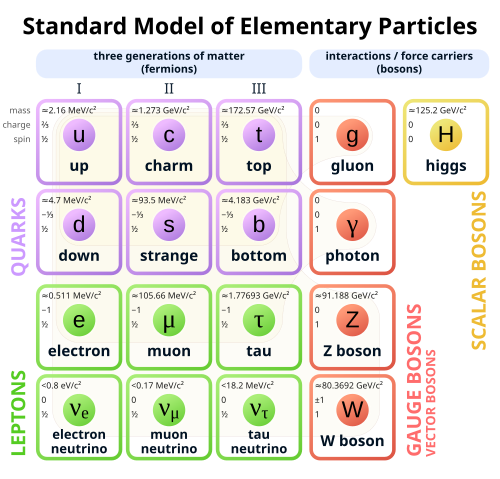
\includegraphics[width=0.6\linewidth]{gallery/background/standard_model.png}
    \caption{Particles of the Standard Model. Figure from \cite{sm}.}
    \label{f.sm}
\end{figure}
%
The particles in the Standard model are tabulated in Fig. \ref{f.sm}. The fermions are the particles which compose all visible matter, and the bosons are the ones which mediate the three fundamental forces between the particles. Nuclear physics is mainly concerned with the strong force, formulated through the theory of quantum chromodynamics (QCD), which describes the interactions between quarks and gluons. The particles which participate in strong-force interactions carry a property known as {\it color charge}, which is analogous to the electric charge in electromagnetism but comes in three values: ``red", ``blue", and ``green". Unlike the photons which mediate the electromagnetic force, the gluons which mediate the strong force also carry color charge themselves. Thus, gluons interact with each other, leading to highly complex and nonlinear dynamics.

%--------------------------
\subsection{The strong coupling constant}

For each force in the Standard Model, there is a characteristic {\it coupling} ``constant" which describes the strength of the associated interactions. For electromagnetism, the coupling is the fine structure constant $\alpha\approx 1/137$, which is a very small number and remains relatively constant across energy scales. In contrast, the strong coupling $\alpha_S$ is large at the low energies of our everyday experience and decreases as energy increases. This leads to the phenomena of {\it color confinement} at low energies and  {\it asymptotic freedom}. Color confinement describes the phenomenon in which the QCD interactions are so strong that at low energies, quarks are always found in color-neutral bound states called {\it hadrons}. Bound states of three quarks, such as protons and neutrons, are known as baryons, and bound states of two quarks (one quark and one antiquark) are known as mesons. On the opposite end of the energy spectrum, {\it asymptotic freedom} describes the phenomenon in which $\alpha_S$ becomes weak enough at high energies to allow quarks and gluons to exist as nearly free particles. This results in the production of quark-gluon plasma, a hot and dense ``soup" of free quarks and gluons, in extremely high energy collisions.

Due to the peculiar behavior of $\alpha_S$, studying the behavior of quarks and gluons within hadrons is challenging. It is impossible to resolve individual quarks and gluons at low energies, and in high energy collisions, we tend to break apart the hadrons we wish to study. Thus, there is still much we do not know about how quarks and gluons are distributed inside of hadrons, and how the hadron properties, such as mass and spin, arise from the interactions of the internal quarks and gluons. In the next section, Ch. \ref{sec.bkg_DIS}, we discuss the process of deep-inelastic scattering, the most common method for studying the structure of protons (and other hadrons).

%---------------------------------------------------------
\section{Imaging the proton through deep-inelastic scattering (DIS)}
\label{sec.bkg_DIS}

We can probe the structure of the proton by scattering an electron beam off a proton target and measuring what happens to the scattered electrons. In general scattering experiments, many measurements relate to an observable known as the cross section $\sigma$, which describes the probability of interaction between the scattering particles. In this section, we introduce the concept of cross sections in high energy experiments, and we discuss how such measurements for deep-inelastic electron-proton scattering can reveal information about proton structure.

%-----------------------------
\subsection{Cross sections in particle physics}
\label{sec.bkg_cross_section}
%
\begin{figure}[h!]
    \centering
    
\includegraphics[width=0.5\linewidth]{gallery/background/cross_section.png}
    \caption{Scattering of two particle beams.}
    \label{f.cross_section}
\end{figure}
%
To illustrate the role of cross sections in particle physics, we follow the discussions in Ch. 14 of {\it A Standard Model Workbook} by Thomas Moore \cite{moore}. Imagine taking a snapshot of two particle beams traveling toward each other, as in Fig. \ref{f.cross_section}. In this snapshot of time interval $T$, beam 1 contains $N_1$ particles, beam 2 contains $N_2$, and their relative velocity is $\mathbf{v}$. Each beam can be approximated by a cylinder of volume $V$ and cross-sectional area $A$. The scattering cross section $\sigma$ relates the flux of incoming particles to the rate of scattering $\Gamma$ per volume,
\begin{equation}
    {\rm flux} \cdot \sigma = \frac{\Gamma}{V} \ .
    \label{eqn.sigma_beam}
\end{equation}

Let us consider the lab frame, in which the particles in beam 2 are at rest and the particles in beam 1 are traveling at $\mathbf{v}$. Here, the length of beam 1 is $|\mathbf{v}|T$. The total incoming flux is
\begin{equation}
    {\rm flux} = \frac{N_1|\mathbf{v}|}{V}\frac{N_2}{V} = \frac{N_1N_2}{AVT} \ ,
    \label{eqn.flux}
\end{equation}
where $N_1|\mathbf{v}|/V = N_1/AT$ is the flux of particles in beam 1, and $N_2/V$ is the density of particles in beam 2. The rate of scattering is
\begin{equation}
    \Gamma = \frac{{\rm Prob}_{1,2\rightarrow1',2'}}{T}N_1N_2,
    \label{eqn.rate}
\end{equation}
where ${\rm Prob}_{1,2\rightarrow1',2'}$ is the probability that a particle from beam 1 and a particle from beam 2 scatter into particles 1' and 2'. Since we are dealing with quantum particles, this probability is given by the squared amplitude for the initial state (particles 1 and 2) transitioning into the final state (particles 1' and 2') via time evolution. Thus, $\Gamma$ is better known as the {\it transition rate}. Additionally, in relativistic high energy collisions, the final state particles may not be the same species as the initial particles. (For example, an electron and positron can annihilate and produce a quark-antiquark pair.)

Substituting Eq. \eqref{eqn.flux} and \ref{eqn.rate} into \ref{eqn.sigma_beam},
\begin{equation}
    \left(\frac{N_1N_2}{VT}\right) \frac{\sigma}{A} = {\rm Prob}_{1,2\rightarrow1',2'}\left(\frac{N_1N_2}{VT}\right) \ .
\end{equation}
Thus, the cross section
\begin{equation}
    \sigma = A \cdot {\rm Prob}_{1,2\rightarrow1',2'}
\end{equation}
represents the effective area of interaction and is directly proportional to the probability of scattering between two particles. 
% For further discussion on this interpretation, Griffiths Ch. 6 \cite{Griffiths} draws a more detailed analogy between $\sigma$ and the Classical cross section through a geometric description of scattering. 

In high energy experiments, we can measure the cross section in terms of {\it luminosity} $\mathcal{L}=N_1N_2/AT$, where
\begin{equation}
    \sigma = \frac{\Gamma}{\mathcal{L}} \ .
\end{equation}
In scattering calculations, we generally work with the slightly more abstract differential cross section
\begin{equation}
    d\sigma = \frac{|\mathcal{M}|^2}{{\rm flux}} d{\rm Lips} \ ,
\end{equation}
where $\mathcal{M}$, called the {\it invariant amplitude}, represents the probability amplitude for the scattering process, and the {\it Lorentz-invariant phase space} $d{\rm Lips}$ represents the density of possible final states. $d{\rm Lips}$ is commonly written in terms of angular coordinates $d\Omega$, energy $dE$, momenta $d^3\mathbf{p}$, or other physical quantities. We say that the cross section is ``differential" in energy, momenta, etc. to indicate that it is measured as a function of such quantities.

% For $2\rightarrow 2$ interactions in which 2 initial particles of four-momenta $p_1$ and $p_2$ scatter into 2 final particles with four-momenta $p_1'$ and $p_2'$, we have a formula known as {\it Fermi's Golden Rule}:
% \begin{equation}
%     d\sigma = S \frac{(2\pi)^4\delta^{(4)}(p_1+p_2-p_1'-p_2') |\mathcal{M}|^2}{4\sqrt{(p_1 \cdot p_2)^2-m_1^2m_2^2}}\frac{d^3\mathbf{p}_1'}{(2\pi)^32E_1'}\frac{d^3\mathbf{p}_2'}{(2\pi)^32E_2'} \ ,
%     \label{eqn.golden_rule}
% \end{equation}

% where
% \begin{equation}
% \begin{aligned}
%     {\rm flux} &= \frac{2E_1|\mathbf{v}|}{V}\frac{2E_2}{V} = \frac{4\sqrt{(p_1 \cdot p_2)^2-m_1^2m_2^2}}{V^2} \\
%     \dot{P} &=\frac{(2\pi)^4\delta^{(4)}(p_1+p_2-p_1'-p_2') |\mathcal{M}|^2}{V^4}  \\
%     dN' &= \frac{Vd^3\mathbf{p}_1'}{(2\pi)^32E_1'}\frac{Vd^3\mathbf{p}_2'}{(2\pi)^32E_2'} \ ,
%     \label{eqn.cross_section_pieces}
% \end{aligned}
% \end{equation}

% where $\mathbf{p}_i$ is the spatial three-momentum of particle $i$ and $m_i^2=p_i^2=E_i^2-|\mathbf{p}_i|^2$ is the mass squared of particle $i$.

% Instead of delving into the derivation of Eq. \eqref{eqn.golden_rule} (which can be found in particle physics textbooks such as Griffiths Ch. 6 \cite{Griffiths} and Moore Ch. 14 \cite{Moore}),
% % and Halzen \& Martin Ch. 4 \cite{Halzen_Martin}), 
% here we provide a qualitative explanation of the important pieces. The most interesting quantity is the invariant amplitude $\mathcal{M}$. This piece contains the process-dependent parts of ${\rm Prob}_{1,2\rightarrow 1',2'}$, thus capturing all the physics of the interaction. The $\delta$-function encodes conservation of four-momentum, requiring that the initial four-momentum $p_1+p_2$ minus the final four-momentum $p_1'+p_2'$ is zero. The factors $d^3\mathbf{p}_i'/(2\pi)^32E'_i$ represent the density of momentum states for each final state particle.
% % All the factors of $2E_i/V$ result from the conventional normalization of incoming and outgoing wavefunctions, which gives $N_i=2E_i$ particles in the total interaction volume $V$. 
% Finally, the factor $S=1/n!$ out front is a degeneracy factor to prevent double-counting, where $n$ is the number of indistinguishable final state particles.
% % (For example, if the final state consists of two electrons, then $S=1/2$.)
% In Ch. \ref{sec.bkg_ep}, we will discuss the cross section for $ep$ scattering processes and how they can capture information about proton structure.

% Imagine taking a snapshot of two particle beams traveling toward each other, as in Fig. \ref{f.cross_section}. In this snapshot of time interval $T$, beam 1 contains $N_1$ particles, beam 2 contains $N_2$, and their relative velocity is $\mathbf{v}$. Each beam can be approximated by a cylinder of volume $V$ and cross-sectional area $A$. The scattering cross section $\sigma$ relates the total number of incoming particles to the number of scattered particles (i.e. the particles that actually interacted),
% \begin{equation}
%     N_{\rm incoming} \cdot \sigma = N_{\rm scattered} \ .
%     \label{eqn.cross_section}
% \end{equation}

% Let us consider the lab frame, in which the particles in beam 2 are at rest and the particles in beam 1 are traveling at $\mathbf{v}$. Here, the length of beam 1 is $|\mathbf{v}|T$. Normalized by the volume and time interval of the interaction, the number of incoming particles is given by
% \begin{equation}
%     \frac{N_{\rm incoming}}{VT} = \frac{N_1|\mathbf{v}|}{V}\frac{N_2}{V} = \frac{N_1N_2}{AVT} \ ,
%     \label{eqn.incoming}
% \end{equation}
% where $N_1|\mathbf{v}|/V = N_1/AT$ is the flux of particles in beam 1, and $N_2/V$ is the density of particles in beam 2. The number of scattering particles is given by
% \begin{equation}
%     \frac{N_{\rm scattered}}{VT} = \dot{P}N_1N_2 = \frac{|S_{fi}|^2}{VT}N_1N_2 \ ,
%     \label{eqn.scattered}
% \end{equation}
% where $\dot{P}=|S_{fi}|^2/VT$ is the scattering probability per volume per time. $S_{fi}$, called the S-matrix element, is the amplitude for the initial states transitioning into the final states through time evolution. As with any quantum process, squaring this amplitude, $|S_{fi}|^2$, gives us the transition probability.

% Substituting equations \ref{eqn.incoming} and \ref{eqn.scattered} into Eq. \eqref{eqn.cross_section},
% \begin{equation}
%     \left(\frac{N_1N_2}{VT}\right) \frac{\sigma}{A} = |S_{fi}|^2\left(\frac{N_1N_2}{VT}\right) \ .
% \end{equation}
% Thus, the cross section $\sigma = A \cdot |S_{fi}|^2$ represents the effective area of interaction and is directly proportional to the scattering probability. In high energy experiments, we measure the cross section in terms of beam luminosity $\mathcal{L}=N_1N_2/AT$ and the total interaction rate $\Gamma_{\rm tot}=N_1N_2\cdot|S_{fi}|^2/T$ \ ,
% \begin{equation}
%     \sigma = \frac{\Gamma_{\rm tot}}{\mathcal{L}} \ .
% \end{equation}

% Generally, we work with the slightly more abstract differential cross section
% \begin{equation}
%     d\sigma = \frac{\dot{P}}{f} dN' \ ,
% \end{equation}
% where $dN'$ is the density of final states and is proportional to angular coordinates $d\Omega$, energy $dE$, or other quantities we can measure. For any $2\rightarrow 2$ interaction in which 2 initial particles of four-momenta $p_1$ and $p_2$ scatter into 2 final particles with four-momenta $p_1'$ and $p_2'$,
% \begin{equation}
%     d\sigma = \frac{1}{n!}\frac{(2\pi)^4\delta^{(4)}(p_1+p_2-p_1'-p_2') |\mathcal{M}|^2}{4\sqrt{(p_1 \cdot p_2)^2-m_1^2m_2^2}}\frac{d^3\mathbf{p}_1'}{(2\pi)^32E_1'}\frac{d^3\mathbf{p}_2'}{(2\pi)^32E_2'} \ ,
%     \label{eqn.diff_cross_section}
% \end{equation}
% where
% \begin{equation}
% \begin{aligned}
%     \dot{P} &= \frac{|S_{fi}|^2}{VT}=(2\pi)^4\delta^{(4)}(p_1+p_2-p_1'-p_2') |\mathcal{M}|^2  \\
%     f &= 2E_1|\mathbf{v}|2E_2 = 4\sqrt{(p_1 \cdot p_2)^2-m_1^2m_2^2} \\
%     \rho &= \frac{d^3\mathbf{p}_1'}{(2\pi)^32E_1'}\frac{d^3\mathbf{p}_2'}{(2\pi)^32E_2'} \ ,
%     \label{eqn.cross_section_pieces}
% \end{aligned}
% \end{equation}
% with $\mathbf{p}_i$ being the spatial three-momentum of particle $i$ and $m_i^2=p_i^2=E_i^2-|\mathbf{p}_i|^2$ being the mass squared of particle $i$. The most interesting quantity in Eq. \eqref{eqn.diff_cross_section} is $\mathcal{M}$, called the invariant amplitude, which is essentially the non-trivial part of $S_{fi}$ and contains all the physics of the interaction. The $1/n!$ out front is a degeneracy factor to prevent double-counting, where $n$ is the number of indistinguishable final state particles. (For the $ep$ scattering processes we will consider, all final state particles will be distinguishable, so $1/n!=1$.) The $\delta$-function piece encodes conservation of four-momentum, requiring that the initial four-momentum $p_1+p_2$ minus the final four-momentum $p_1'+p_2'$ is zero. We will not delve further into the derivations for the expressions in Eq. \eqref{eqn.cross_section_pieces}, but these can be found in particle physics textbooks such as Griffiths Ch. 6 \cite{Griffiths} and Aitchison \& Hey Ch. 6 \cite{Aitchison_Hey}. In the next subsection \ref{sec.bkg_ep}, we will discuss the invariant amplitude $\mathcal{M}$ for various $ep$ scattering processes.

%-----------------------------
\subsection{Elastic $e\mu$ scattering: a first look at Feynman diagrams}
\label{sec.bkg_feynman}
Before delving into the details $ep$ scattering, let us first introduce {\it Feynman diagrams}, an essential tool for calculating cross sections in particle physics, and the common kinematic variables (Ch. \ref{sec.bkg_emu}). As an example, we will consider a simpler but related process: elastic electron-muon scattering $e^-\mu^-\rightarrow e^-\mu^-$.

%
\begin{figure}[h!]
    \centering
    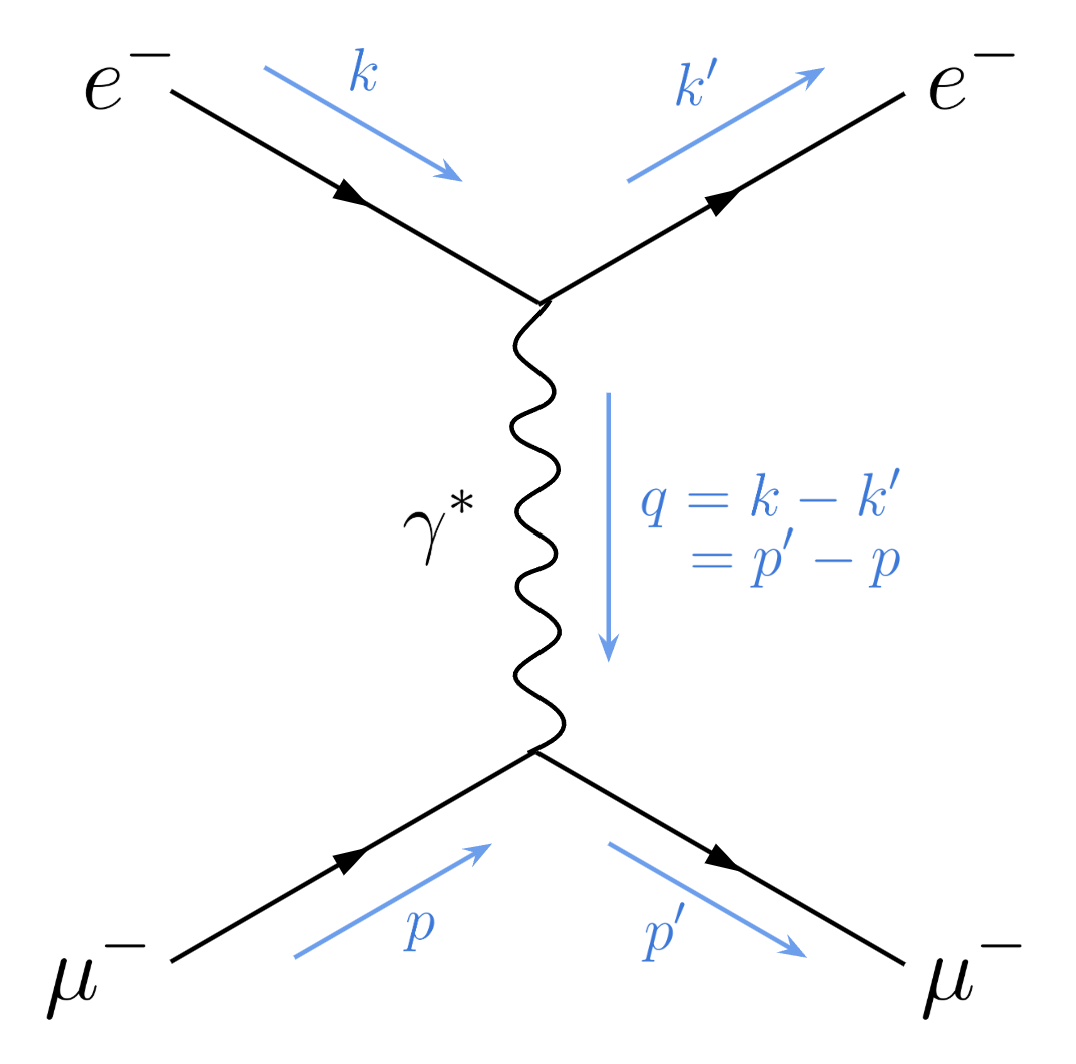
\includegraphics[width=0.4\linewidth]{gallery/background/emu_emu.png}
    \caption{Leading order Feynman diagram for elastic electron-muon scattering, $e^-(k) + \mu^-(p) \rightarrow e^-(k') + \mu^-(p')$. Four-momenta are labeled in blue.}
    \label{f.emu_emu}
\end{figure}
%
The Feynman diagram for the $e\mu$ scattering is shown in Fig. \ref{f.emu_emu}. We read the diagram from left to right, with the initial state particles on the left and final state particles on the right. Conventionally, fermions like electrons and muons are drawn as 
\begin{tikzpicture}
\begin{feynman}
\diagram {
  a -- [fermion] b
};
\end{feynman}
\end{tikzpicture} \ ,
and photons are drawn as 
\begin{tikzpicture}
\begin{feynman}
\diagram {
  a -- [photon] b
};
\end{feynman}
\end{tikzpicture} \ .
These particle lines are called {\it propagators}. The blue arrows in Fig. \ref{f.emu_emu} denote the four-momentum of each particle. (A four-momentum is an object that combines the energy $E$ and three-dimensional momentum vector $\mathbf{p}$ into a single vector, $p\equiv(E,\mathbf{p})=(E,p_x,p_y,p_z)$. For more background on four-momenta and four-vectors, see Appendix \ref{sec.relativity}). 

Altogether, the diagram depicts an electron with four-momentum $k$ and a muon with four-momentum $p$ traveling toward each other, exchanging a photon with four-momentum $q$, then scattering off with new four-momenta $k'$ and $p'$. We can see that this is an electrodynamic interaction, since it is mediated by the exchange of a photon.

To clarify, Feynman diagrams do not illustrate what the interaction physically looks like in space, so we should avoid interpreting the particles as interacting at some location or at some particular time. Instead, the diagrams serve as mathematical tools for calculating cross sections. From quantum field theory, there are a set of {\it Feynman rules} that associate a specific factor with every vertex and propagator, which multiply together to produce an expression for the invariant amplitude $\mathcal{M}$.

%
\begin{figure}[h!]
    \centering
    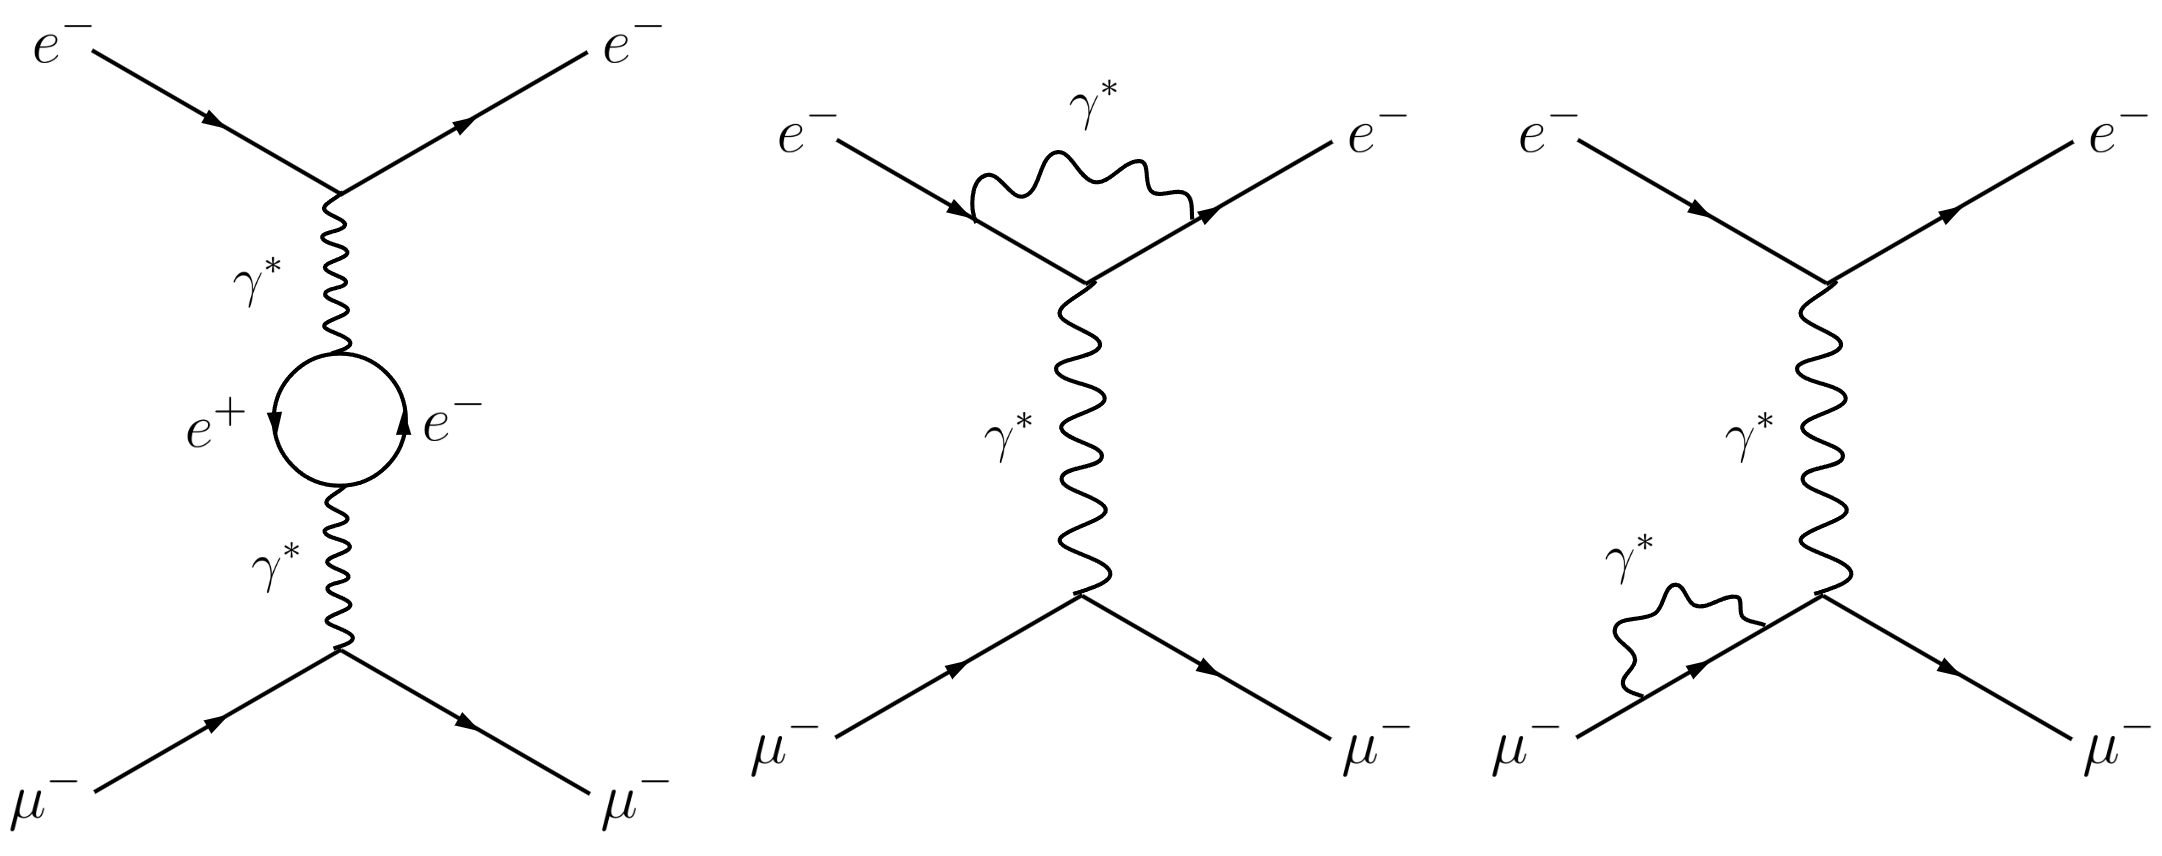
\includegraphics[width=0.8\linewidth]{gallery/background/emu_nlo.png}
    \caption{Examples of next-to-leading order Feynman diagrams for $e^-\mu^-\rightarrow e^-\mu^-$.}
    \label{f.emu_nlo}
\end{figure}
%
Actually, Fig. \ref{f.emu_emu} is the first term in an infinite series of Feynman diagrams for $e
\mu$ scattering, and the true invariant amplitude $\mathcal{M}$ is the sum of all their contributions. We refer to Fig. \ref{f.emu_emu} as the {\it leading order} diagram, which means that it contains the lowest number of vertices (two in this case) needed for the interaction to occur. All other diagrams are of higher order, containing more vertices. Fig. \ref{f.emu_nlo} shows a few examples of Feynman diagrams for $e\mu$ scattering at next-to-leading order, which all involve four vertices.

The Feynman rules tell us that every vertex comes with a factor proportional to the {\it electromagnetic coupling}, $\alpha=e^2/4\pi\approx1/137$, which determines the interaction strength in electrodynamic processes. Summing all the possible diagrams, we have
\begin{equation}
    \mathcal{M} = \mathcal{M}^{(1)}(\alpha^2) + \mathcal{M}^{(2)}(\alpha^4) + \mathcal{M}^{(3)}(\alpha^8) + \cdots \ ,
\end{equation}
where $\mathcal{M}^{(i)}$ is the $i$-th term in a {\it perturbative} expansion in powers of $\alpha^2$. Since the value of $\alpha$ is very small ($\alpha^2\approx5.3\times10^{-5}\ll1$), higher-order terms become progressively smaller ($\mathcal{M}^{(i+1)}\ll \mathcal{M}^{(i)}$), so they act like incremental corrections (or perturbations) to the previous terms. For electrodynamic processes like $e\mu$ scattering, the leading order term alone is enough to give a reasonable approximation of $\mathcal{M}$.

%-----------------------------
\subsection{Elastic $e\mu$ scattering: the lab frame view}
\label{sec.bkg_emu}

In these next sections, Ch. \ref{sec.bkg_emu}-\ref{sec.bkg_dis_partons}, we walk through the pedagogical approach of Francis Halzen and Alan Martin in {\it Quarks and Leptons} \cite{Halzen_Martin} to develop our understanding of deep-inelastic scattering from the starting point of $e\mu$ scattering.

%
\begin{figure}[h!]
    \centering
    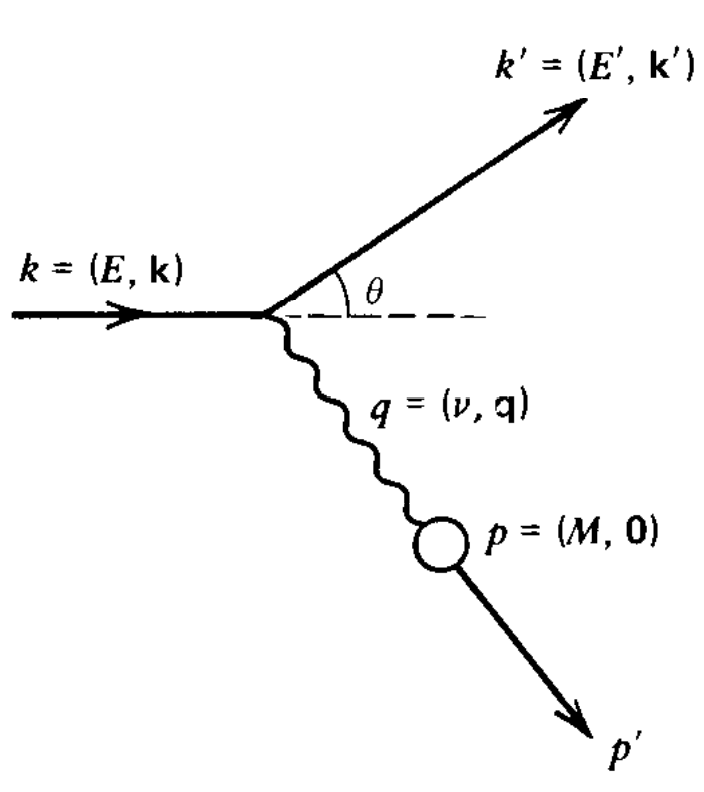
\includegraphics[width=0.4\linewidth]{gallery/background/emu_lab.png}
    \caption{Cartoon depiction of $e^-\mu^-\rightarrow e^-\mu^-$ scattering in the lab frame. Figure from Halzen \& Martin \cite{Halzen_Martin}.}
    \label{f.emu_lab}
\end{figure}
%
In determining particle collisions and cross-sections, our main objective is to calculate the invariant amplitude $\mathcal{M}$, which encodes the physics of the interaction. Since $\mathcal{M}$ is Lorentz-invariant, we can choose a reference frame that is easy to work with. One common choice is the lab frame, in which the muon is initially at rest. We can also assume that the electron mass is negligible, i.e. $m_e\approx 0$, since it is much smaller than all other energy scales in the interaction. Fig. \ref{f.emu_lab} illustrates how this interaction looks in the lab frame. The electron hits a stationary muon, then scatters off at an angle $\theta$ with respect to its initial direction of motion. A photon is exchanged, transferring some four-momentum from the electron to the muon, which then recoils. The four-momenta are
\begin{center}
\begin{equation}
\begin{aligned}
    & k = (E,\mathbf{k}) \\ 
    & k' = (E,\mathbf{k'}) \\
    & q \equiv (\nu, \mathbf{q}) = k-k' \\
    & p = (M,\mathbf{0}) \\ 
    & p' = p+q \ ,
    \label{eqn.k_p_q}
\end{aligned}
\end{equation}
\end{center}
where $M$ is the muon mass. It follows from the relativistic mass-energy-momentum relation, $m^2=E^2-|\mathbf{p}|^2$, that if the electron is approximately massless, $E^2\approx|\mathbf{k}|^2$ and $(E')^2\approx|\mathbf{k'}|^2$. Then $\mathbf{k}\cdot\mathbf{k'}=|\mathbf{k}||\mathbf{k'}|\cos{\theta}\approx EE'\cos{\theta}$.

Let us bring our attention to the exchanged photon. Unlike the electron and muon, which are {\it external} particles, the photon does not appear in the initial nor final state, but is a completely {\it internal} propagator. Its role is to mediate the interaction, carrying four-momentum between the electron and muon. In other words, the amount of four-momentum transferred from the electron to the muon, $q\equiv(\nu, \mathbf{q})=k-k'$, is precisely the four-momentum of the photon. (By conservation of four-momentum, we also have $q=p'-p$.) We can calculate $q^2$ in the lab frame:
\begin{equation}
\begin{aligned}
    q^2 &= (k-k')^2 \\
    &= k^2 + (k')^2 - 2k\cdot k' \\
    &= 2m_e^2 - 2 k\cdot k' \\
    &\approx -2k\cdot k' \ ,
\end{aligned}
\end{equation}
where $k^2=(k')^2=m_e^2\approx0$ by the relativistic mass-energy-momentum relation. Then by definition of the dot product between four-momenta, $k\cdot k'\equiv EE'-\mathbf{k}\cdot\mathbf{k'}$, and
\begin{equation}
\begin{aligned}
    q^2 &= -2(EE'-|\mathbf{k}||\mathbf{k'}|\cos{\theta}) \\
    &\approx -2EE'(1-\cos{\theta}) \ .
\end{aligned}
\end{equation}
% (For more details about manipulating four-momenta, see Appendix \ref{sec.relativity}.)

We find that $q^2$ is in general nonzero,
% Thus, $q^2\neq m_\gamma^2$, seemingly breaking the laws of relativity. Vaguely speaking, the Heisenberg uncertainty principle $\Delta E \Delta t \geq 1 / 2$ provides some leeway, allowing such particles to fluctuate into existence for an extremely brief, unobservable, amount of time. 
meaning $q^2\neq m_\gamma^2$. (Although we performed the calculation in the lab frame, $q^2$ is Lorentz-invariant, so its value is the same in every reference frame.) This photon does not obey the relativistic mass-energy-momentum relationship, and therefore it must be fundamentally unobservable. Such particles are termed {\it virtual}, or {\it off-shell}. In general, all internal propagators are virtual particles. (They are sometimes labeled with a $*$ symbol, like $\gamma^*$ in Fig. \ref{f.emu_emu}.)

In processes like $e^-\mu^-\rightarrow e^-\mu^-$, we use the square of the four-momentum transfer, $q^2$ to quantify the energy of the scattering interaction. Since $q^2<0$, we define the positive variable 
\begin{equation}
    Q^2 \equiv -q^2 \ .
\end{equation} 
In Ch. \ref{sec.bkg_dis_dsigma}-\ref{sec.bkg_dis_partons}, we will apply these kinematics to examine $ep$ scattering.

%-----------------------------
% \subsection{$ep$ scatterings and proton structure}
% \label{sec.bkg_ep}
% %
% In this section, we will discuss the cross sections of $ep$ scattering interactions and how they relate to proton structure....

% %
% \begin{figure}[h!]
%     \centering
%     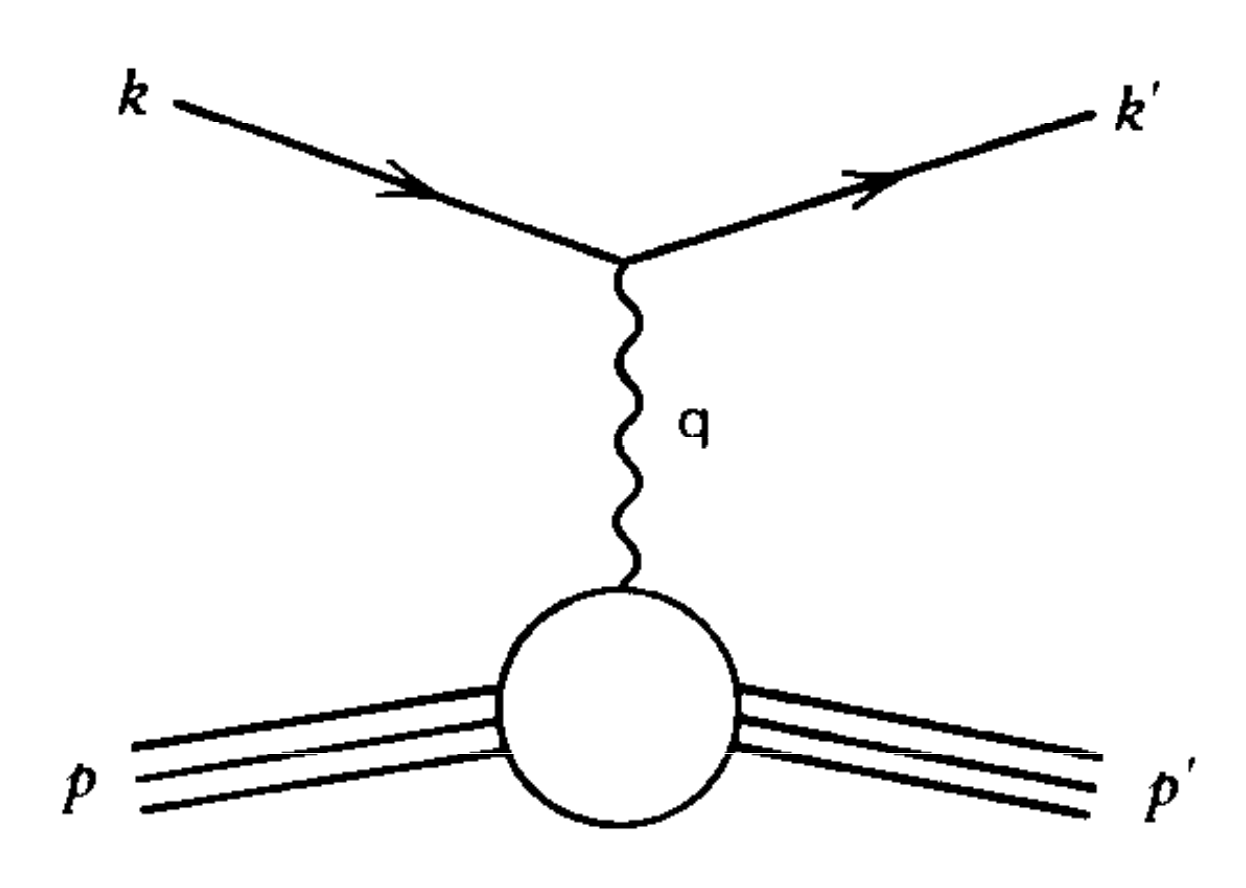
\includegraphics[width=0.5\linewidth]{gallery/background/ep_ep.png}
%     \caption{Leading order Feynman diagram for elastic electron-proton scattering, $e^-(k) + p(p) \rightarrow e^-(k') + p(p')$. Figure from Halzen \& Martin \cite{Halzen_Martin}.}
%     \label{f.ep_ep}
% \end{figure}
% %
% The Feynman diagram for $e^-+p\rightarrow e^-+p$, shown in Fig. \ref{f.ep_ep}, has the same general structure as the diagram for $e^-+\mu^-\rightarrow e^-+\mu^-$ in Fig. \ref{f.emu_emu}. In fact, the top half of the diagrams, which deals with the electron, are identical. However, in the bottom half of Fig. \ref{f.ep_ep}, we now have a proton, which is a complex hadron composed of quarks and gluons. We draw the proton propagator with multiple lines and the proton-photon vertex as a blob, representing the ambiguity about what the particles are inside the proton and how they interact with the photon. In the following discussion, we will parametrize how the proton, being a particle with nontrivial structure, affects the scattering cross section.

% As for the $e\mu$ scattering example in Ch. \ref{sec.bkg_emu}, let us consider the $ep$ scattering in the lab frame, with the proton is initially at rest, and assume that the electron is approximately massless. The $ep$ interaction looks exactly like the illustration in Fig. \ref{f.emu_lab}, with the same four-momenta as those listed in Eq. \eqref{eqn.k_p_q}. 
% % The electron travels toward the proton with initial four-momentum $k=(E,\mathbf{k})$, exchanges a virtual photon with four-momentum $q\equiv(\nu,\mathbf{q})=k-k'$, then scatters off with a new four-momentum $k'=(E',\mathbf{k'})$ such that $\mathbf{k}\cdot \mathbf{k'}=|\mathbf{k}||\mathbf{k'}| \cos{\theta}=EE'\cos{\theta}$. The proton has an initial four-momentum $p=(M,\mathbf{0})$, where $M$ is its mass, and recoils with final four-momentum $p'=p+q$.

% If the proton were a point particle, like the muon, then the differential cross section would be
% \begin{equation}
%     \left(\frac{d\sigma}{d\Omega} \right)_{\rm point} = \left( \frac{\alpha}{2E\sin^2\frac{\theta}{2}} \right)^2 \frac{E'}{E} \left[ \cos^2\frac{\theta}{2}-\frac{q^2}{2M^2}\sin^2\frac{\theta}{2} \right] \ ,
%     \label{eqn.ep_ep_point}
% \end{equation}
% where $d\Omega=r^2\sin{\theta}drd\theta d\phi$ is the solid-angle where the scattered particles are measured, $\theta$ is the polar angle with respect to the particle beam axis (the $z$-axis), and $\alpha$ is the electromagnetic coupling. $k=(E,\mathbf{k})$ is the four-momentum of the incoming electron, $k'=(E',\mathbf{k'})$ is that of the outgoing electron, and $q=(\nu,\mathbf{q})$ is that of virtual photon (see Eq. \eqref{eqn.k_p_q}).

% However, because the proton has some structure, the cross section is given by the more complicated {\it Rosenbluth formula}:
% \begin{equation}
%     \left(\frac{d\sigma}{d\Omega} \right)_{ep\rightarrow ep} = \left( \frac{\alpha}{2E\sin^2\frac{\theta}{2}} \right)^2 \frac{E'}{E} \left[ {\color{purple}\frac{G_E^2(q^2)+\tau G_M^2(q^2)}{1+\tau} }\cos^2\frac{\theta}{2}-{\color{purple}2\tau G_M^2(q^2)}\sin^2\frac{\theta}{2} \right] \ ,
%     \label{eqn.ep_ep_dsigma}
% \end{equation}
% where $M$ is the proton mass, $\tau=-q^2/4M^2$, and $G_E(q^2)$ and $G_M(q^2)$ are two independent functions of $q^2$. The function $G_E$ and $G_M$ essentially modify Eq. \eqref{eqn.ep_ep_point} to account for the effects of proton structure on the scattering interaction. At leading order, $e^-+p\rightarrow e^-+p$ is also an electrodynamic interaction, since it is mediated by a virtual photon. Thus, $G_E$ and $G_M$ are called the electric and magnetic {\it form factors}. They encode information about the electric charge density and magnetic current density of the proton, which we can probe through elastic $ep$ scattering experiments.

%-----------------------------
\subsection{Deep-inelastic scattering: the $ep\rightarrow eX$ cross section}
\label{sec.bkg_dis_dsigma}
In 1969, Richard Feynman proposed the idea that nucleons are composed of point-like {\it partons}, which we now identify as the quarks and gluons of the Standard Model.
In this section and the next, we discuss the characteristics of deep-inelastic scattering (DIS) and how such experiments allow us to probe the partons within the proton. 

% In general, $ep$ collisions can be elastic, with the electron and proton scattering off each other similarly to $e^-\mu^-\rightarrow e^-\mu^-$. They can also be inelastic, in which the proton breaks apart and new particles are produced. The most relevant interaction for this work is deep-inelastic scattering (DIS), $ep\rightarrow eX$ (where $X$ represents any particles).

%
\begin{figure}[h!]
    \centering
    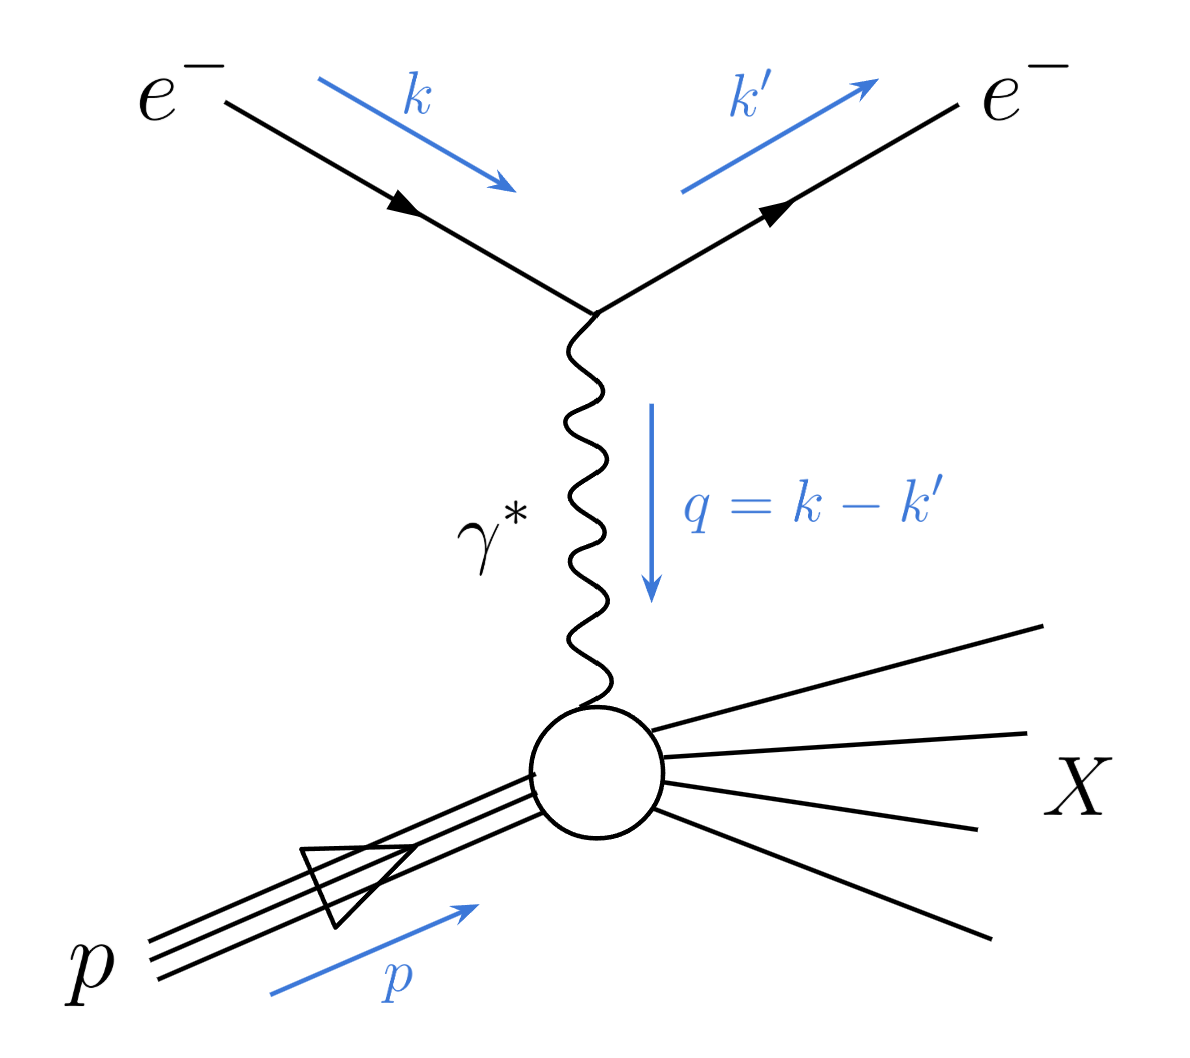
\includegraphics[width=0.4\linewidth]{gallery/background/ep_eX.png}
    \caption{Leading order Feynman diagram for the inelastic scattering $e^-(k) + p(p) \rightarrow e^-(k') + X$. Four-momenta are labeled in blue.}
    \label{f.ep_eX}
\end{figure}
%
The leading order Feynman diagram for DIS, $ep\rightarrow eX$ (where $X$ refers to any particles), is shown in Fig. \ref{f.ep_eX}. The process is similar to that for $e^-\mu^-\rightarrow e^-\mu^-$ in Fig. \ref{f.emu_emu}. In fact, the top half of the diagrams, which deals with the electron, are identical. In the bottom half, we now have an incoming proton, which is subsequently broken up during the interaction, and an array of new particles $X$ is produced.

Unlike the muon, the proton is a complex hadron with internal structure. We draw the proton propagator with multiple lines and its interaction vertex as a blob to represent ambiguity about what exactly the particles are inside the proton and how they interact. In order to examine proton structure, it is not necessary to measure all the particles produced, and we simply denote them collectively as $X$. We refer to such measurements as {\it inclusive}, meaning that we remain agnostic about the final state particles $X$ and, in our calculations, simply sum over all the possible final states. (Measurements can also be semi-inclusive, if we measure one or a few of the particles produced.)

As we did for the $e\mu$ scattering example in Ch. \ref{sec.bkg_emu}, let us consider $ep\rightarrow eX$ in the lab frame, with the proton is initially at rest, and assume that the electron is approximately massless. If the proton were a point particle, the interaction would look exactly like the illustration in Fig. \ref{f.emu_lab}, with the same four-momenta as those listed in Eq. \eqref{eqn.k_p_q}. 
% For the electron,
% \begin{equation}
% \begin{aligned}
%     k &= (E,|\mathbf{k}|) \\
%     k' &= (E'|\mathbf{k'}|) \ ,
% \end{aligned}
% \end{equation}
% with $\mathbf{k}\cdot\mathbf{k'}\approx EE'(1-\cos{\theta})$. For the virtual photon,
% \begin{equation}
%     q=(\nu, \mathbf{q}) = k-k' ,
% \end{equation}
% and for the proton,
% \begin{equation}
% \begin{aligned}
%     p &=(M,\mathbf{0}) \\
%     p' &= p+q \ ,
% \end{aligned}
% \end{equation}
% where $M$ is the proton mass.
The differential cross section would be \cite{Halzen_Martin}
\begin{equation}
    \left(\frac{d\sigma}{d\Omega dE'} \right)_{\rm point} = \left( \frac{\alpha}{2E\sin^2\frac{\theta}{2}} \right)^2 \frac{E'}{E} \left[ \cos^2\frac{\theta}{2}+\frac{Q^2}{2M^2}\sin^2\frac{\theta}{2} \right] \delta\left(\nu - \frac{Q^2}{2M} \right) \ ,
    \label{eqn.ep_point}
\end{equation}
where $d\Omega=r^2\sin{\theta}drd\theta d\phi$ is the solid-angle where the scattered particles are measured, $\theta$ is the polar angle with respect to the particle beam axis (the $z$-axis), and $\alpha$ is the electromagnetic coupling. $k=(E,\mathbf{k})$ is the four-momentum of the incoming electron, $k'=(E',\mathbf{k'})$ is that of the outgoing electron, and $q=(\nu,\mathbf{q})$ is that of the virtual photon, with $Q^2=-q^2$. The delta-function $\delta\left(\nu -{Q^2}/{2M} \right)$ restricts the values of the photon energy to $\nu=Q^2/2M$.

However, because the proton has some structure, the differential cross section involves a bit more complexity \cite{Halzen_Martin}:
\begin{equation}
    \left(\frac{d\sigma}{d\Omega dE'} \right)_{\rm DIS} = \left( \frac{\alpha}{2E\sin^2\frac{\theta}{2}} \right)^2 \frac{E'}{E} \left[ {\color{purple}\frac{F_2(Q^2,\nu)}{\nu}}\cos^2\frac{\theta}{2}-{\color{purple}\frac{2F_1(Q^2,\nu)}{M}}\sin^2\frac{\theta}{2} \right] \ ,
    \label{eqn.ep_eX}
\end{equation}
where $F_1$ and $F_2$ are {\it structure functions} that modify Eq. \eqref{eqn.ep_point} to account for the effects of proton structure on the scattering interaction. In addition, $\nu$ is now independent of $Q^2$, as reflected by the absence of the delta-function term.

%-----------------------------
\subsection{Deep-inelastic scattering: from proton to partons}
\label{sec.bkg_dis_partons}
What do the structure functions $F_1$ and $F_2$ reveal about the proton? In the $ep\rightarrow eX$ Feynman diagram of Fig. \ref{f.ep_eX}, we can think of the virtual photon as our probe into the proton. For very high energy collisions, the energy of the photon is large, so its wavelength is small. Thus, the higher the energy, the smaller the distance scales the experiment can resolve. In the regime of deep-inelastic scattering, the energy is high enough for the photon to probe individual partons. 

In fact, in the {\it Bjorken limit}, in which $Q^2\rightarrow\infty$ and $\nu\rightarrow\infty$ while their ratio remains finite, we can model DIS as elastic scatterings of the electron with a single quark inside the proton. In this regime, $F_1$ and $F_2$ no longer scale separately with $Q^2$ and $\nu$, but only depend on the ratio
\begin{equation}
    x \equiv \frac{Q^2}{2M\nu} \ , \label{eqn.bjorken}
\end{equation}
called {\it Bjorken-$x$}.

% To interpret this Bjorken-$x$ variable, let us consider deep-inelastic scattering $ep$ scattering in the limit where the motion of all particles is along the particle beams. 
% This is known as the infinite-momentum frame, in which the proton has momentum $|\mathbf{p}|\equiv p_z\rightarrow\infty$. In this limit, all partons inside the proton have such large momenta in the $z$-direction, that we can assume their motion to be collinear to the proton and neglect any transverse momentum.
%
\begin{figure}[h!]
    \centering
    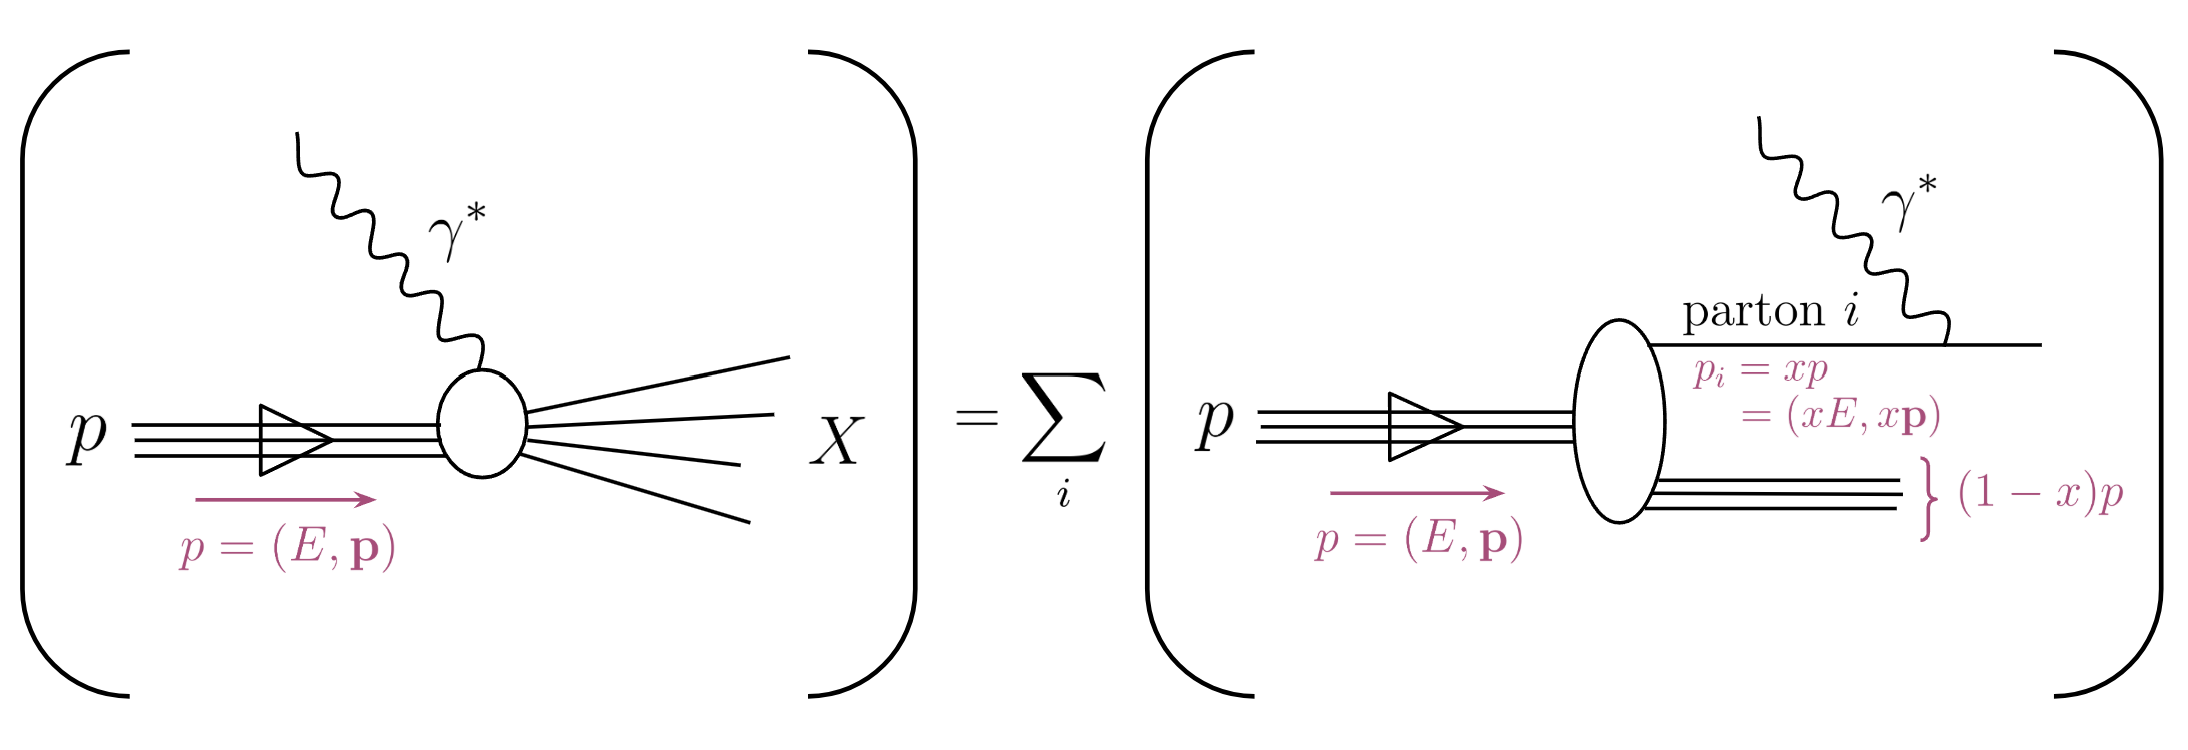
\includegraphics[width=0.95\linewidth]{gallery/background/ep_parton.png}
    \caption{Cartoon depiction of the $\gamma^*p$ interaction in $ep\rightarrow eX$ as the sum of $\gamma^*$-parton interactions in the infinite momentum frame. Four-momenta are labeled in magenta. Figure adapted from Halzen \& Martin \cite{Halzen_Martin}.}
    \label{f.ep_parton}
\end{figure}
%
Figure \ref{f.ep_parton} depicts the $\gamma^*p$ interaction in $ep\rightarrow eX$ (the lower half of Fig. \ref{f.ep_eX}) as the sum of all possible interactions between $\gamma^*$ and a parton $i$ inside the proton. (For simplicity, let us assume all partons are traveling in the same direction as the proton.) For a proton with four-momentum $p=(E,\mathbf{p})$, a given parton $i$ has four-momentum $p_i=xp$. In other words, Bjorken-$x$ is the parton {\it momentum fraction}, the fraction of the proton momentum carried by a given parton. 

The structure functions are given by \cite{Halzen_Martin}
\begin{equation}
    2xF_1(x) = F_2(x) = \sum_i e_i^2xf_i(x) \ ,
    \label{eqn.F1_F2}
\end{equation}
where $e_i$ is the electric charge of parton $i$ in units of the proton charge (e.g. $e=2/3$ for up quarks, $e=-1/3$ for down quarks, and $e=0$ for gluons), and $f_i(x)$ is known as the {\it parton distribution function}. The parton distribution function, defined by
\begin{equation}
\begin{aligned}
    dP_i &= f_i(x) \ dx \\
    1 = \sum_idP_i &= \sum_i \int_0^1 f_i(x) \ dx \ ,
    \label{eqn.pdf}
\end{aligned}
\end{equation}
is the probability density of finding a parton of flavor $i$ with momentum fraction $x$. In other words, $f_i(x)$ describes the momentum-space distribution of partons inside the proton. (Technically, only the quarks contribute to Eq. \eqref{eqn.F1_F2}, since gluons have no electric charge. The gluons contribute to $ep\rightarrow eX$ through higher order terms, such as in the photon-gluon fusion process in Fig. \ref{f.ccbar}.)

Beyond the collinear parton distribution functions (PDFs) described in Eq. \eqref{eqn.pdf}, a variety of more complex observables have been formulated to capture various aspects of quark and gluon dynamics. For example, transverse-momentum dependent (TMD) PDFs account for both the collinear and transverse motion of partons, generalized parton distributions (GPDs) describe the parton distributions in three-dimensional position-space, and polarized versions of these functions describe the distribution of spin among the partons \cite{pdfs}.


% We can check that this parton model makes some sense if we consider the $x\rightarrow 1$ limit (as if the proton were one large parton). If $x=1$ and $e=1$ (the proton charge), then $f(x)=1$ and $\nu=Q^2/2M$ (see Eq. \eqref{eqn.bjorken}), which means 
% \begin{equation}
% \begin{aligned}
%     F_2(x) &= 1 \\
%     2F_1(x) &= \frac{1}{x} = \frac{2M\nu}{Q^2}
% \end{aligned}
% \end{equation}
% This reduces Eq. \eqref{eqn.ep_eX} for the $ep\rightarrow eX$ cross section to Eq. \eqref{eqn.ep_point}, the cross section for a hypothetical point-like proton.

%---------------------------------------------------------
\section{The Electron-Ion Collider (EIC) and the search for Color Glass Condensate (CGC)}
\label{sec.bkg_EIC}

The Electron-Ion Collider (EIC) \cite{EIC} is a new particle collider currently being built at Brookhaven National Lab, designed to image protons and nuclei with unprecedented precision. Through high energy deep-inelastic scattering experiments with electron-proton ($ep$) and electron-ion ($eA$) collisions, the EIC will reveal detailed information about the spatial and momentum distributions of quarks and gluons within protons and nuclei. Measurements of these various parton distributions will bring us closer to understanding the complex dynamics responsible for the generation of mass and spin in nuclear matter.

In particular, the high energies of the EIC will allow us to more effectively study the gluons, which are thought to carry significant contributions to proton mass and spin, yet whose distributions and dynamics are much less understood than those of the quarks. One major phenomena of interest is the existence of a {\it Color Glass Condensate (CGC)}, a theorized state of nuclear matter characterizing the internal structure of protons at very high energies. In this high energy regime---or more precisely, in the regime of small Bjorken-$x$ (defined in Eq. \eqref{eqn.bjorken})---proton structure is dominated by gluons. This is because gluons, being massless particles that can self-interact due to their color charge, will tend to split into more gluons with infinitesimal momentum fraction, forming a highly dense ``condensate" of ``colored" bosons. However, when two gluons meet, they can also recombine into a single gluon, so the gluon density cannot continue to grow unchecked as Bjorken-$x$ approaches 0. Eventually, the rate of gluon splitting ($g\rightarrow gg$) and recombination ($gg\rightarrow g$) will reach an equilibrium, causing the gluon density to {\it saturate}. Additionally, because the gluons are also extremely time-dilated after being accelerated to high energies, they form Classical ``glass"-like fields that evolve very slowly in time. 

Previous experiments at the HERA Collider at DESY in Germany, operational from 1992 to 2007, found signatures consistent with the presence of Color Glass Condensate, but the data did not extend to low enough Bjorken-$x$ to observe true gluon saturation. At the EIC, which is set to begin operations in the 2030s, one overarching goal is to obtain more direct evidence of saturation and study the dynamics of the CGC.

%---------------------------------------------------------
\section{Heavy flavor probes}
\label{sec.bkg_heavy_flavor}

%
\begin{figure}[h!]
    \centering
    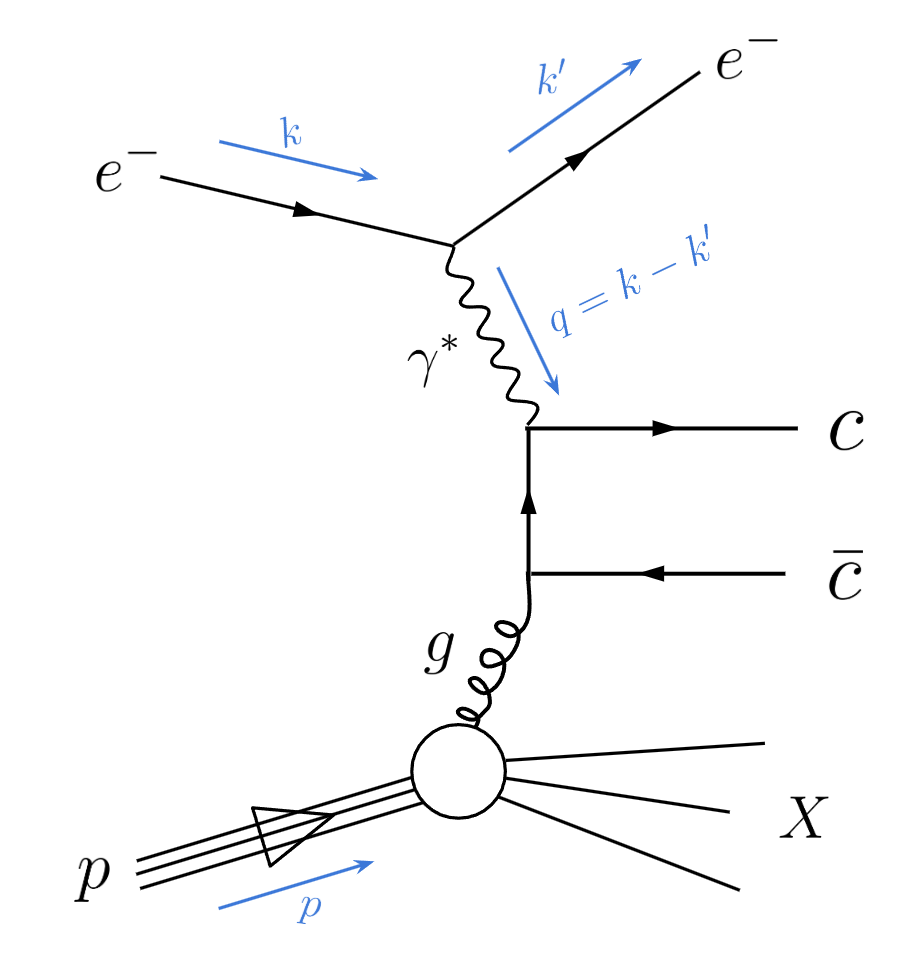
\includegraphics[width=0.4\linewidth]{gallery/background/ccbar.png}
    \caption{Photon-gluon fusion in deep-inelastic scattering, leading to the production of a charm and anti-charm pair.}
    \label{f.ccbar}
\end{figure}
%
During electron-proton and electron-ion collisions at the EIC, interactions involving gluons can lead to the production of {\it heavy flavor} quarks: charm ($c$) and beauty ($b$). The most common of such processes is photon-gluon fusion, depicted in Fig. \ref{f.ccbar}, in which the electron emits a virtual photon, which then interacts with a gluon inside a proton (or neutron) to produce a quark-antiquark pair. Because heavy flavor quarks are so massive, they can only be produced in gluon interactions during the initial high-energy $ep$ collisions. (The masses are around $1~{\rm GeV/c^2}$ for $c$ and $4~{\rm GeV/c^2}$ for $b$, vs. only $1~{\rm GeV/c^2}$ and $5~{\rm GeV/c^2}$ for the most common $u$ and $d$ quarks, respectively.) Thus, heavy flavor quarks carry information about the initial collision conditions, serving as high-sensitivity probes to the gluon distributions and dynamics we wish to study.

After being produced, quarks will immediately hadronize into color-neutral bound states. Consequently, we must study heavy flavor quarks through the hadrons they form, such as the $D^0$-meson, which is the subject of this analysis. In Chapter \ref{ch:d0_top}, we will discuss our method of analyzing these short-lived $D^0$-mesons in $ep$ collisions at the EIC.
\chapter{Topology of the $D^0 \rightarrow \pi+K$ decay}
\label{ch:d0_top}

This chapter begins our discussion of the work conducted for this thesis. Here, we first discuss the topology of the $D^0\rightarrow\pi+K$ decay, which we use to distinguish true $D^0$ signals from background. We introduce the topological variables in Ch. \ref{sec.d0_intro}-\ref{sec:def_top_vars}, then examine the distributions of these variables and their dependence on $D^0$ kinematics in Ch. \ref{sec.d0_kinematics}. Finally in Ch. \ref{sec.d0_strategy}, we outline our plan for utilizing these topological distributions in our $D^0$ analysis.

All of the data used in this thesis come from PYTHIA-8 simulations of $ep$ collisions, provided by the ePIC Collaboration (ref. in Appendix \ref{app.samples}).

%------------------------------------------------------
\section{$D^0$ production and decay}
\label{sec.d0_intro}

In high energy experiments, such as electron-proton collisions at the EIC, charm quarks are produced and hadronize into heavy flavor particles. $D^0$-mesons, containing one charm quark and one up quark, are the lightest and thus most abundant of these heavy flavor particles. However, the $D^0$ cannot be directly detected due to their short lifetime and neutral electric charge. Thus, we must reconstruct the $D^0$ from the tracks left by its decay daughters. In this analysis, we focus on the $D^0 \rightarrow \pi+K$ decay channel, in which a $D^0$-meson decays into a pair of oppositely charged pion and kaon daughters, either $\pi^++K^-$ or $\pi^-+K^+$. Fig. \ref{f.ep_d0_pik} provides a cartoon illustration to summarize this channel of $D^0$ production and decay.
%
\begin{figure}[h!]
    \centering
    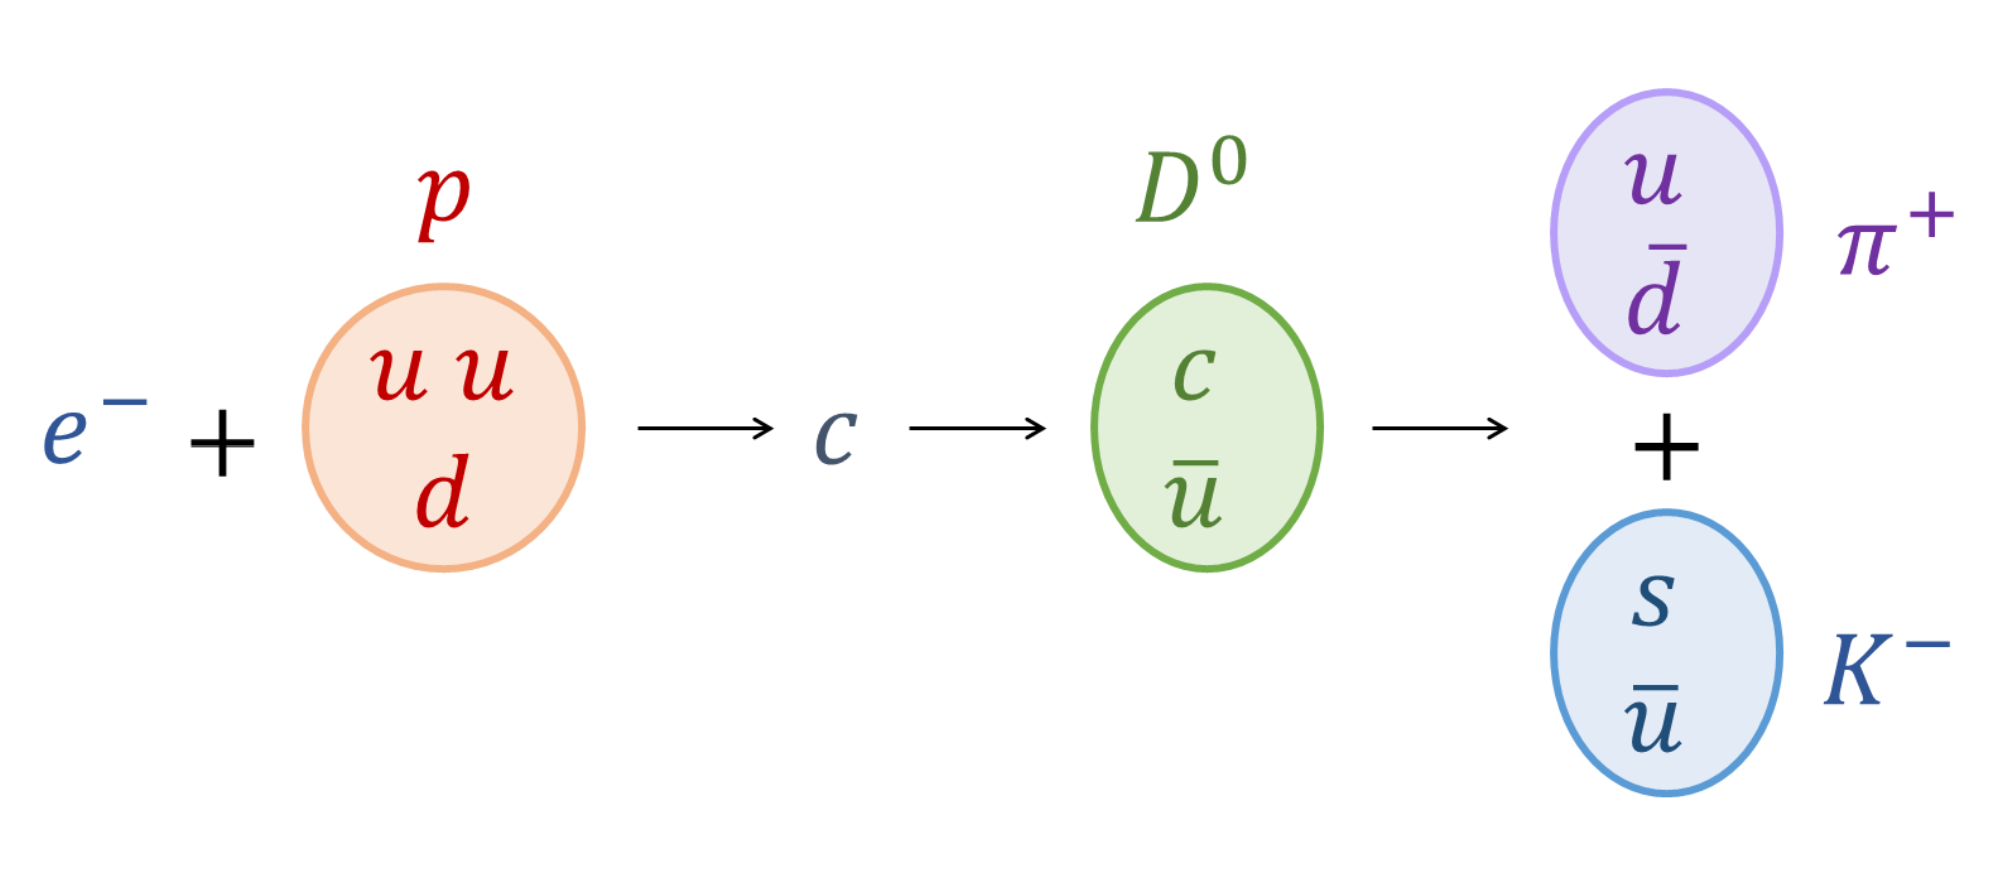
\includegraphics[width=0.7\linewidth]{gallery/D0_topology/ep_d0_pik.png}
    \caption{Production and decay of a $D^0$-meson in an $ep$ collision.}
    \label{f.ep_d0_pik}
\end{figure}
%

A major challenge in reconstructing $D^0$-mesons is identifying the correct $\pi K$ pairs. Pions and kaons, being the lightest hadrons, are constantly produced through a variety of processes. In contrast, due to the high mass of the charm quark (1.27 GeV/c$^2$), heavy flavor particles like the $D^0$ are rarely produced. Consequently, most of the measured pions and kaons do not originate from a $D^0$ decay, and random $\pi K$ combinations form a large {\it background} that can obscure the true $D^0$ signals we are looking for.

Fortunately, the $D^0\rightarrow \pi+K$ decay occurs with a specific {\it topology}, or geometric pattern, which we can leverage to distinguish $D^0$ signals from background. If we measure the topological variables associated with each reconstructed $\pi K$ pair, we can expect the distributions of true $D^0$-decayed pairs to look different from those of random background pairs. The strategy then is to apply a set of {\it topological cuts}, or selection criteria on the topological variables, to help separate the signal and background candidates. 

%------------------------------------------------------
\section{Topological variables defined}
\label{sec:def_top_vars}

Fig. \ref{f.d0_decay_diagram} depicts the particle trajectories associated with $D^0 \rightarrow \pi+K$ in the transverse plane, forming the two-dimensional decay topology. The {\it primary vertex} marks the location at which the $ep$ collision occurs and the $D^0$ is produced. The $D^0$ travels for some distance and then decays at the $D^0$ decay vertex, a type of {\it secondary vertex}. The pion and kaon daughters then travel away from the decay vertex, their paths bent in opposite directions due to the presence of a magnetic field. Passing through the detectors, they leave hits that are fitted into tracks (represented by the solid blue curves.)

%
\begin{figure}[h!]
    \centering
    \includegraphics[width=0.6\linewidth]{gallery/D0_topology/d0_decay.png}
    \caption{$D^0\rightarrow \pi^+ + K^-$ decay in the transverse plane. Solid blue lines indicate the directly detected pion and kaon tracks. Dashed lines indicate reconstructed particle trajectories. Figure from the STAR Collaboration \cite{STAR}.}
    \label{f.d0_decay_diagram}
\end{figure}
%

Based on knowledge of the magnetic field strength and particle momenta, we can extrapolate the detected $\pi K$ tracks backward in space and time (dashed curves), forming a {\it helix} trajectory for each particle. (The transverse trajectories are circular due to the magnetic field, but motion in the $z$-direction is constant. Thus in three-dimensions, the particle paths are helical.) We then measure the {\it distance of closest approach (DCA)} between the $\pi K$ pair (${\rm DCA}_{12}$), defined as the perpendicular distance between the two helices, and reconstruct the $D^0$ decay vertex at the midpoint. The primary vertex is reconstructed similarly, but using particles originating from the initial $ep$ collision. Using conservation of momentum, we can also reconstruct the $D^0$ momentum vector $\overrightarrow{P}$. Since the $D^0$ is electrically neutral, its trajectory is a straight line in the direction of $\overrightarrow{P}$.

Following a previous $D^0$ analysis by the STAR Collaboration \cite{STAR}, we use the following topological variables to characterize the $D^0\rightarrow\pi+K$ decay:
\begin{itemize}
    \item ${\rm DCA}_{12}$: distance of closest approach between $\pi K$ pair
    \item ${\rm DCA_\pi}$: distance of closest approach of $\pi$ to primary vertex
    \item ${\rm DCA_K}$: distance of closest approach of $K$ to primary vertex
    \item ${\rm DCA_{D0}}$: distance of closest approach of $D^0$ (or $\overrightarrow P$) to primary vertex
    \item Decay Length: distance between primary vertex and secondary vertex
    \item $\theta$: angle between $\overrightarrow{P}$ and the line connecting primary vertex to secondary vertex
\end{itemize}
Note that Fig. \ref{f.d0_decay_diagram} visualizes the decay topology projected onto the transverse plane, so all variables in the picture are technically the two-dimensional components, ${\rm DCA}_{{\rm \pi}{(xy)}}$,  ${\rm DCA}_{{\rm K}{(xy)}}$, $\theta_{xy}$, etc.


%------------------------------------------------------
\section{Dependence of topological variables on $D^0$ kinematics}
\label{sec.d0_kinematics}

%--------------------------
\subsection{Kinematic variables: rapidity ($y$) and transverse momentum ($p_T$)}
\label{sec:dep_of_top_dists}
%
\begin{figure}[h!]
    \centering
    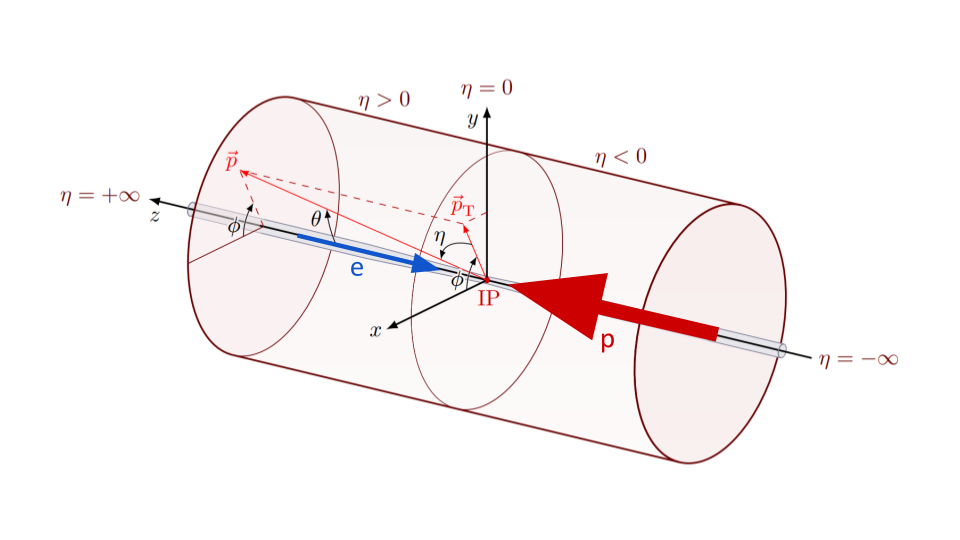
\includegraphics[width=0.65\linewidth]{gallery/D0_topology/coordinates.png}
    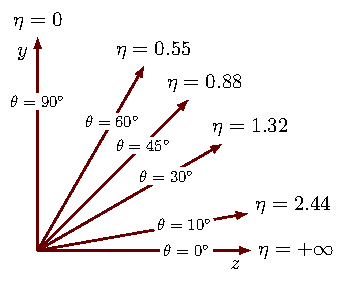
\includegraphics[width=0.3\linewidth]{gallery/D0_topology/pseudorapidity.pdf}
    \caption{Coordinate system for collider experiments. The red arrow indicates the proton beam, and the blue arrow indicates the electron beam, both pointing in the particles' direction of travel. Figures adapted from \cite{tikz}.}
    \label{f.coordinates}
\end{figure}
%
In high energy collisions, particles are accelerated to relativistic speeds. Thus, we describe their motion using a ``relativistic version" of velocity known as {\it rapidity}  (see Appendix \ref{sec.relativity}), defined
\begin{align}
    y \equiv \tanh^{-1}(v_z)\equiv \frac{1}{2}\ln \left[ \frac{E+p_z}{E-p_z} \right] \ , \label{eqn.rapidity}
\end{align}
where $v_z$ is the velocity of the particle, $E$ is its total energy, and $p_z$ is its momentum. By convention, we take the particles' direction of motion to be along the $z$-axis, which defines the beam axis. In $ep$ collisions, we define the proton beam to travel toward the $(+z)$-direction, or the forward direction, and the electron beam to travel toward the $(-z)$-direction, or the backward direction.

In high energy experiments, we measure the closely related {\it pseudorapidity},
\begin{equation}
    \eta \equiv -\ln\left[\tan\left(\frac{\theta}{2}\right) \right] \equiv \frac{1}{2}\ln \left[\frac{|\mathbf{p}|+p_z}{|\mathbf{p}|-p_z} \right] \ ,
\end{equation}
where $\theta$ is the polar angle with respect to the beam axis, and $\mathbf{p}$ is the three-dimensional momentum vector of a particle. The pseudorapidity has a nice geometric interpretation, as depicted in Fig. \ref{f.coordinates}. Particles with $\eta \approx 0$ are detected in the central region of the collision and have $p_L\approx0$. Particles with $\eta>0$ are found in the forward region while particles with $\eta<0$ are found in the backward region, with larger $|\eta|$ being closer to the ends of the collision region and corresponding to larger $|p_z|$. For particles traveling near the speed of light, $E\gg m$. They become near-massless, $|\mathbf{p}|\approx E$, and thus $\eta \approx y$. In this thesis, we use the terms ``pseudorapidity" and ``rapidity" interchangeably.

{\color{brown} Define/introduce transverse momentum.}

%
\begin{figure}[h!]
    \centering
    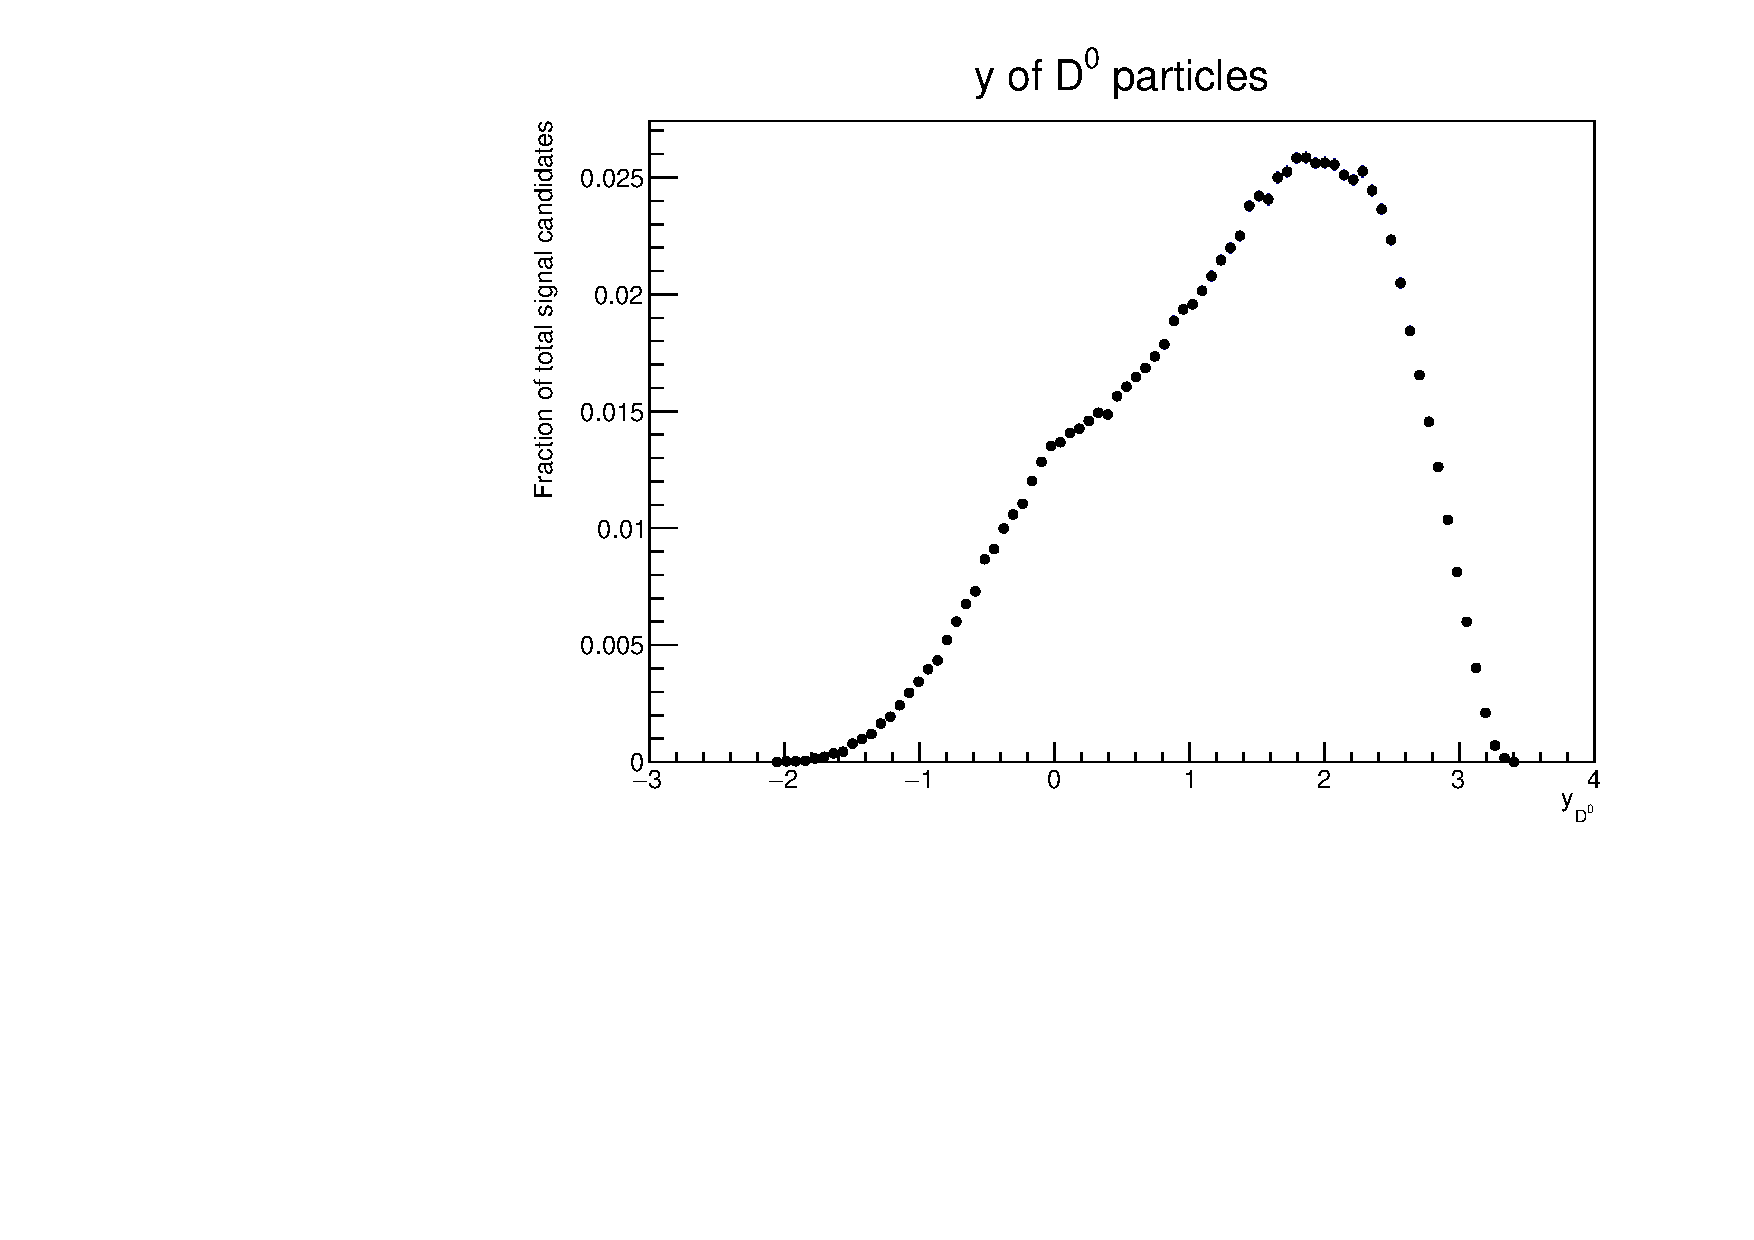
\includegraphics[width=0.45\linewidth]{gallery/D0_topology/D0_y.pdf}
    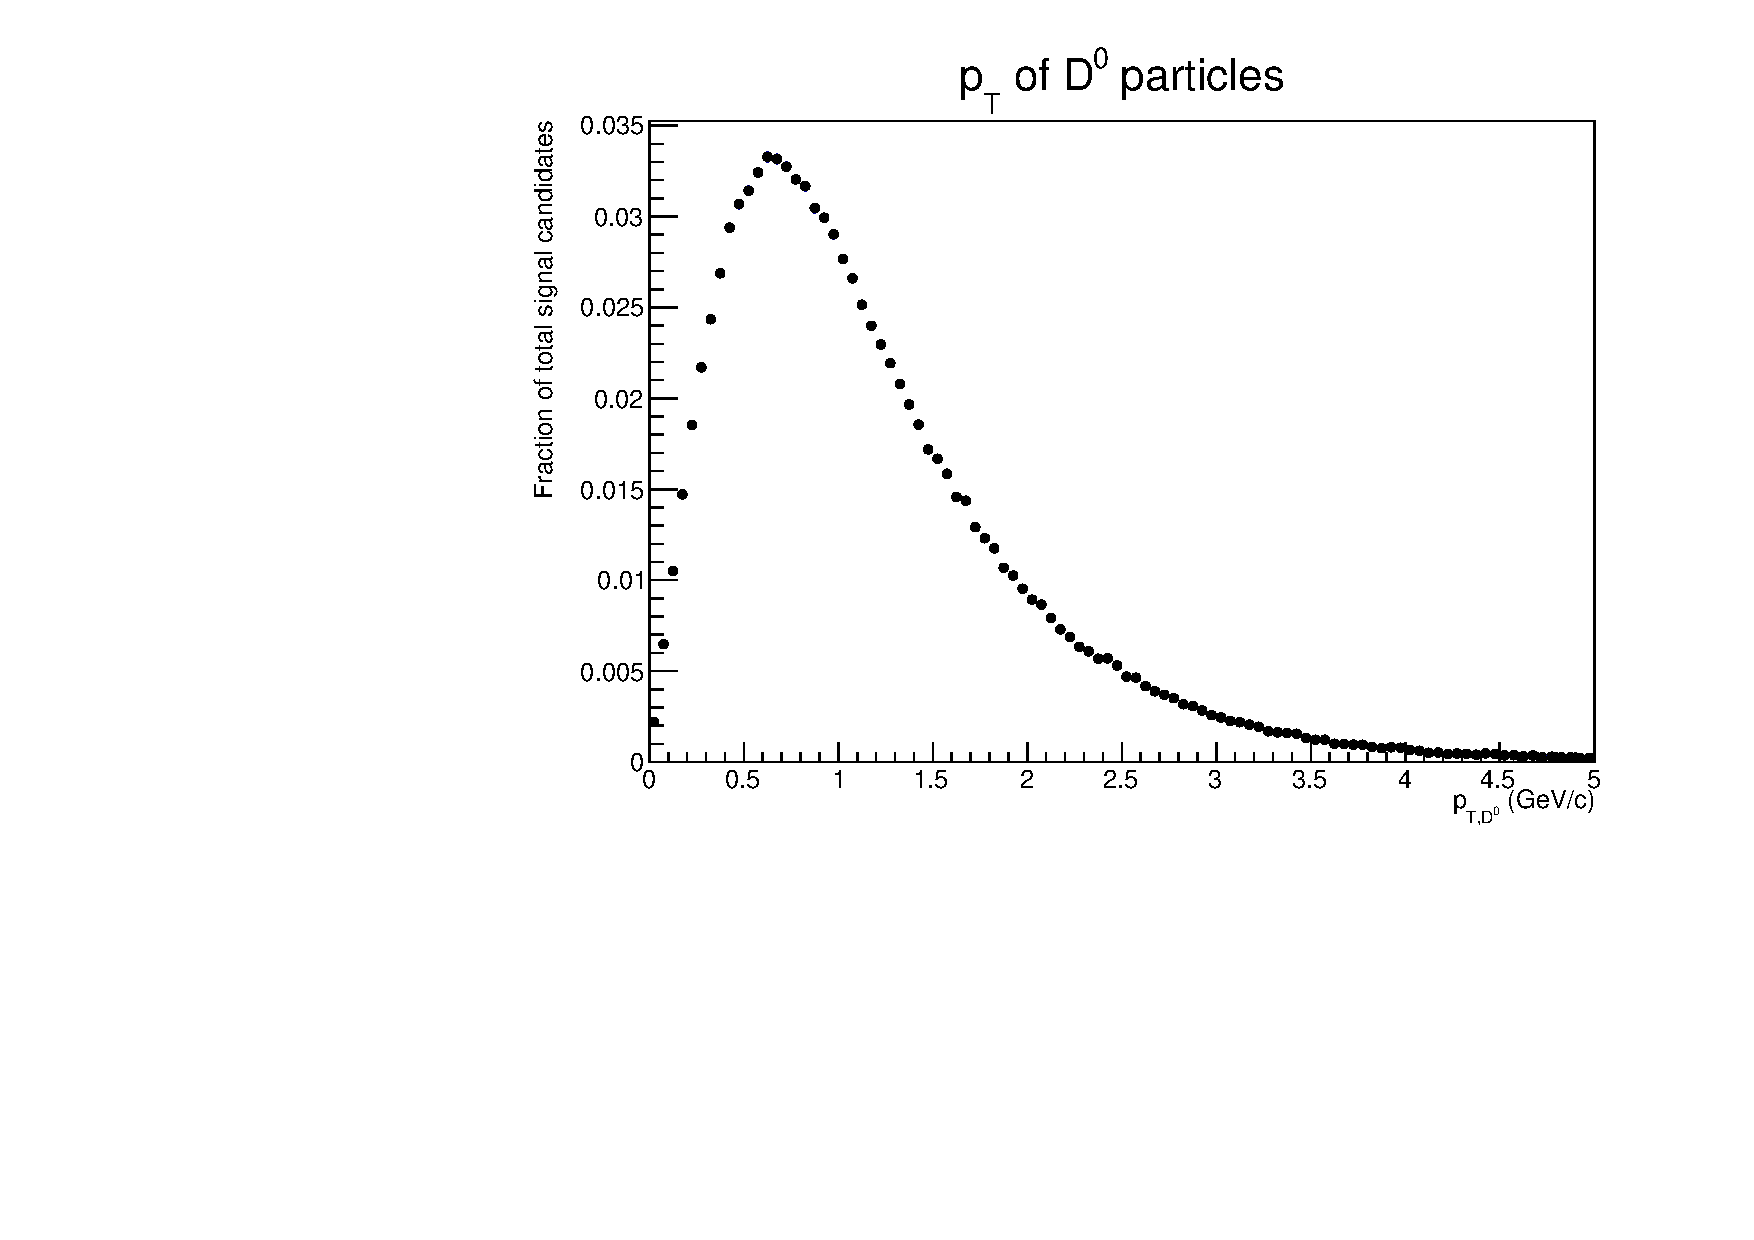
\includegraphics[width=0.45\linewidth]{gallery/D0_topology/D0_pT.pdf}
    \caption{Rapidity ($y$) and transverse momentum ($p_T$) distributions of reconstructed $D^0$-mesons in simulated $ep$ collisions with $Q^2>1~\text{GeV}^2$.}
    \label{f.y_pT}
\end{figure}
%
Fig. \ref{f.y_pT} shows the $y$ and $p_T$ distributions of $D^0$-mesons produced in simulated $ep$ collisions with $Q^2>1$. Here, it is interesting to see that the $y$ distribution is skewed toward the forward (positive) side, reflecting the asymmetry of the collision system. Because the proton has much more mass ($0.938~{\rm GeV/c^2}$) than the electron ($0.511~{\rm GeV/c^2}$), the net momentum is in the proton's direction of motion. Thus, most particles are produced at forward rapidity, with $y>0$ and $\eta>0$. The $p_T$ distribution peaks near $0.7~{\rm GeV/c}$ then falls off, with relatively few $D^0$-mesons exhibiting $p_T>2~{\rm GeV/c}$.

% We divide the analysis into  mid-rapidity $-1<y~(\eta)<1$ and forward rapidity $1<y~(\eta)<3$. However, the shapes of the $D^0 \rightarrow \pi+K$ topological distributions (as we will see in the next section \ref{sec.top_y_pt_slices}).

% Fig. \ref{f.y_pT} also shows the $p_T$ distributions of the $D^0$-mesons, which peaks around 0.7 GeV/c. High-$p_T$ $D^0$-mesons, which results in high-$p_T$ pions and kaons, travel with straighter trajectories and are therefore more easily reconstructed.  

%--------------------------
\subsection{$D^0$ topological distributions in various $y$ and $p_T$ slices}
\label{sec.top_y_pt_slices}

Let us first consider how we might expect the $D^0\rightarrow\pi+K$ topology to depend on $y$ and $p_T$ of the $D^0$. From a physics perspective, the $D^0$ momentum affects its lifetime and the trajectories of its $\pi K$ daughters. According to special relativity, $D^0$-mesons with a larger momentum (or velocity) experience greater time dilation, which means that they travel farther before decaying. Furthermore, the $\pi K$ daughters will also have larger momenta, which means that their trajectories are less bent by the magnetic field. Thus, we can expect higher $p_T$ to be correlated with larger decay length and smaller ${\rm DCA_\pi}$ and ${\rm DCA_K}$.

In addition to the physics, there are also reconstruction effects at play. In general, because higher $p_T$ tracks are straighter, they can be fitted and extrapolated with better precision. As for rapidity, detector performance tends to be better at mid-$y$ (mid-$\eta$), far away from the particle beams, so reconstruction is also better at mid-rapidity compared to forward and backward rapidity. Thus, high $p_T$ and mid-$y$ yield the most accurate and precise results. For the $D^0 \rightarrow\pi+K$ topology, this could mean smaller ${\rm DCA}_{12}$, ${\rm DCA_{D0}}$, and $\theta$ in these regions. (If reconstruction were perfect, then these values would be 0, since the $D^0$ should originate at the primary vertex and decay at the decay vertex, where the pion and kaon then originate together.)
%
\begin{figure}[h!]
    \centering
    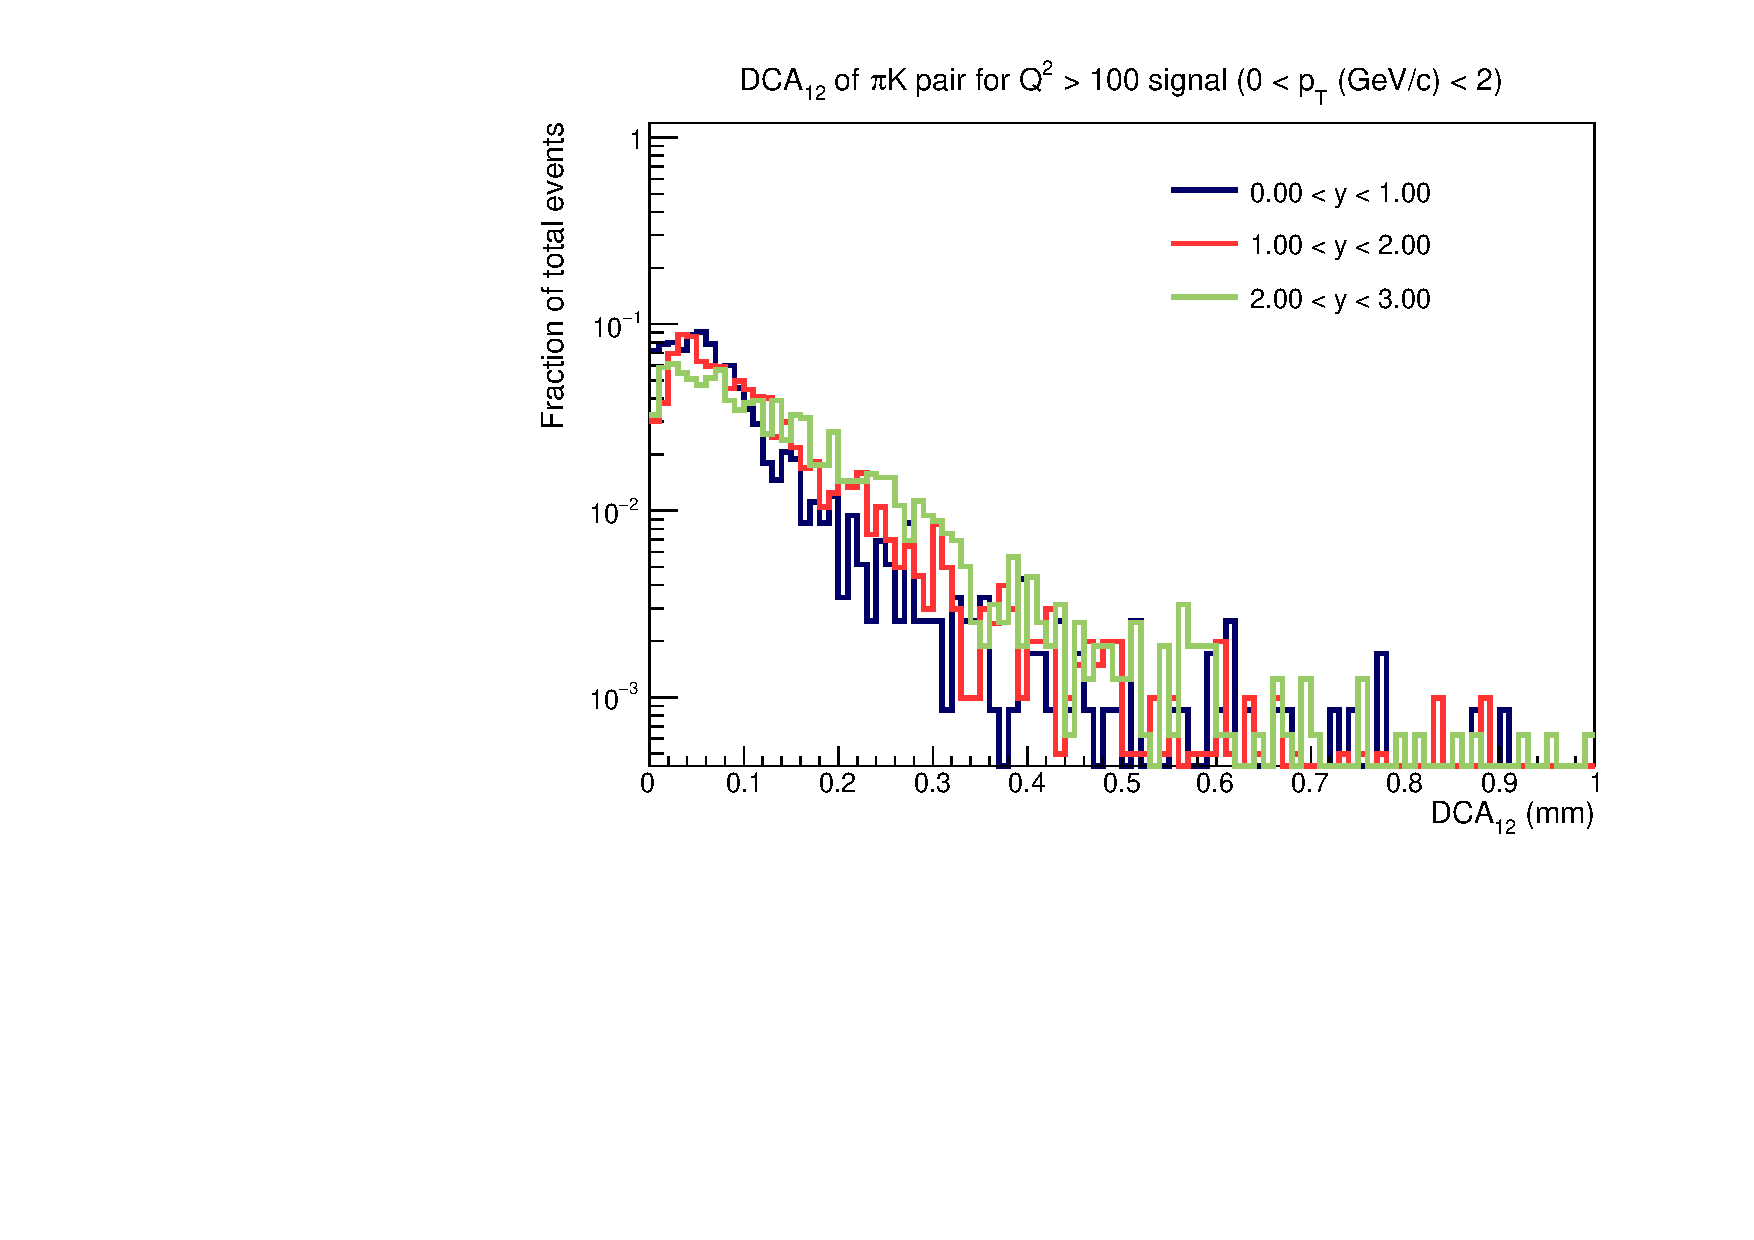
\includegraphics[width=0.55\linewidth]{gallery/D0_topology/DCA12_by_y.pdf}
    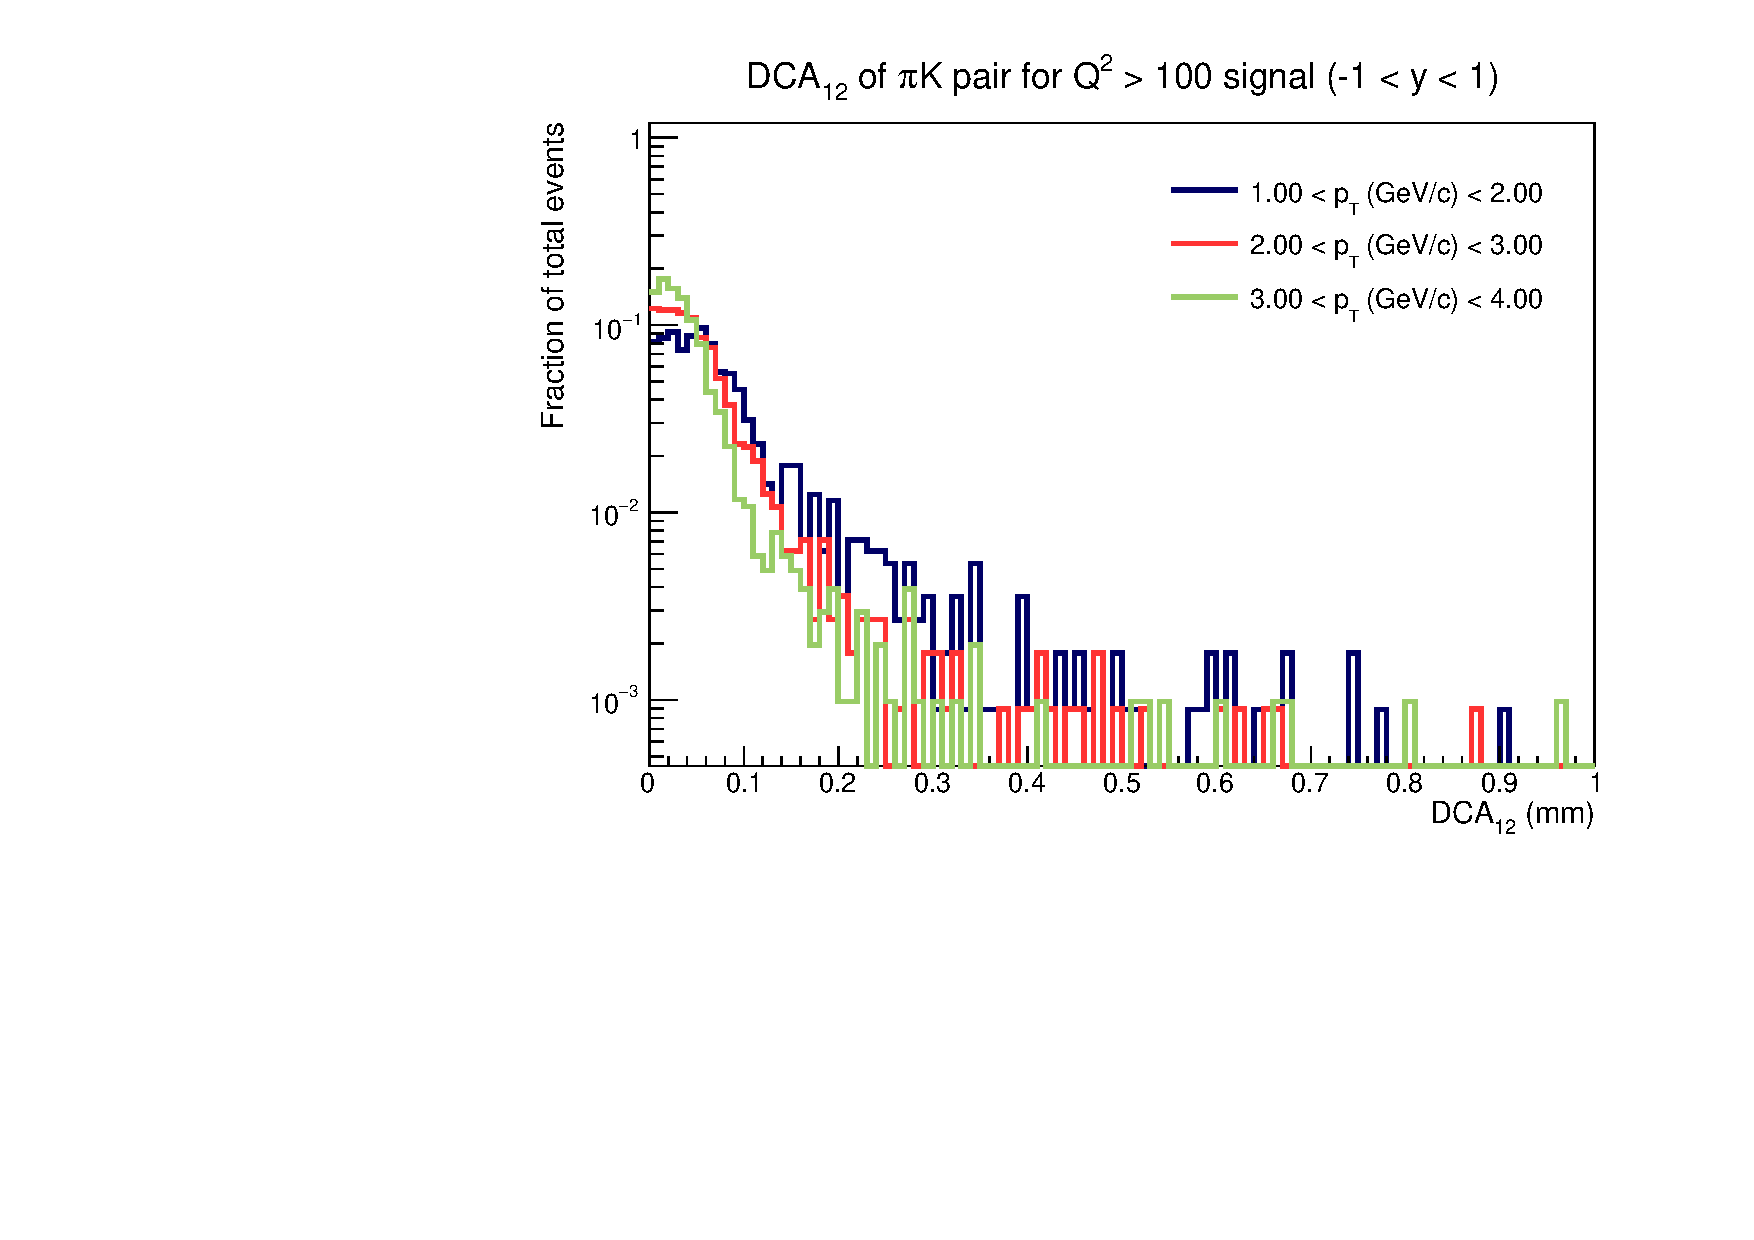
\includegraphics[width=0.55\linewidth]{gallery/D0_topology/DCA12_by_pt.pdf}
    \caption{Examples of the $y$- and $p_T$-dependence of $\text{DCA}_{12}$ of reconstructed $D^0$-mesons in simulated $Q^2>100~\text{GeV}^2$ $ep$ collisions. The top plot compares distributions in various $y$ ranges for $0<p_T<2$ GeV/c, and the bottom plot compares distributions in various $p_T$ ranges for $-1<y<1$.}
    \label{f.top_by_y_pt}
\end{figure}
%

With these effects in mind, we examined the topological variables for reconstructed $D^0$-mesons from simulated $ep$ collisions in different slices of $y$ and $p_T$.  Fig. \ref{f.top_by_y_pt} illustrates these kinematic dependences for the $\text{DCA}_{12}$. As expected, we observe that forward $y$ (green line in the top plot) and low $p_T$ (blue line in the bottom plot) result in wider distributions, which indicate a larger degree of uncertainty in the true value of the topological variables in these regions. This suggests worsening reconstruction performance as we move toward forward $y$ low $p_T$. The distributions for ${\rm DCA_{D0}}$, ${\rm DCA_{\pi}}$, ${\rm DCA_{K}}$, and $\theta$ exhibit the same trends, as expected.

%
\begin{figure}[h!]
    \centering
    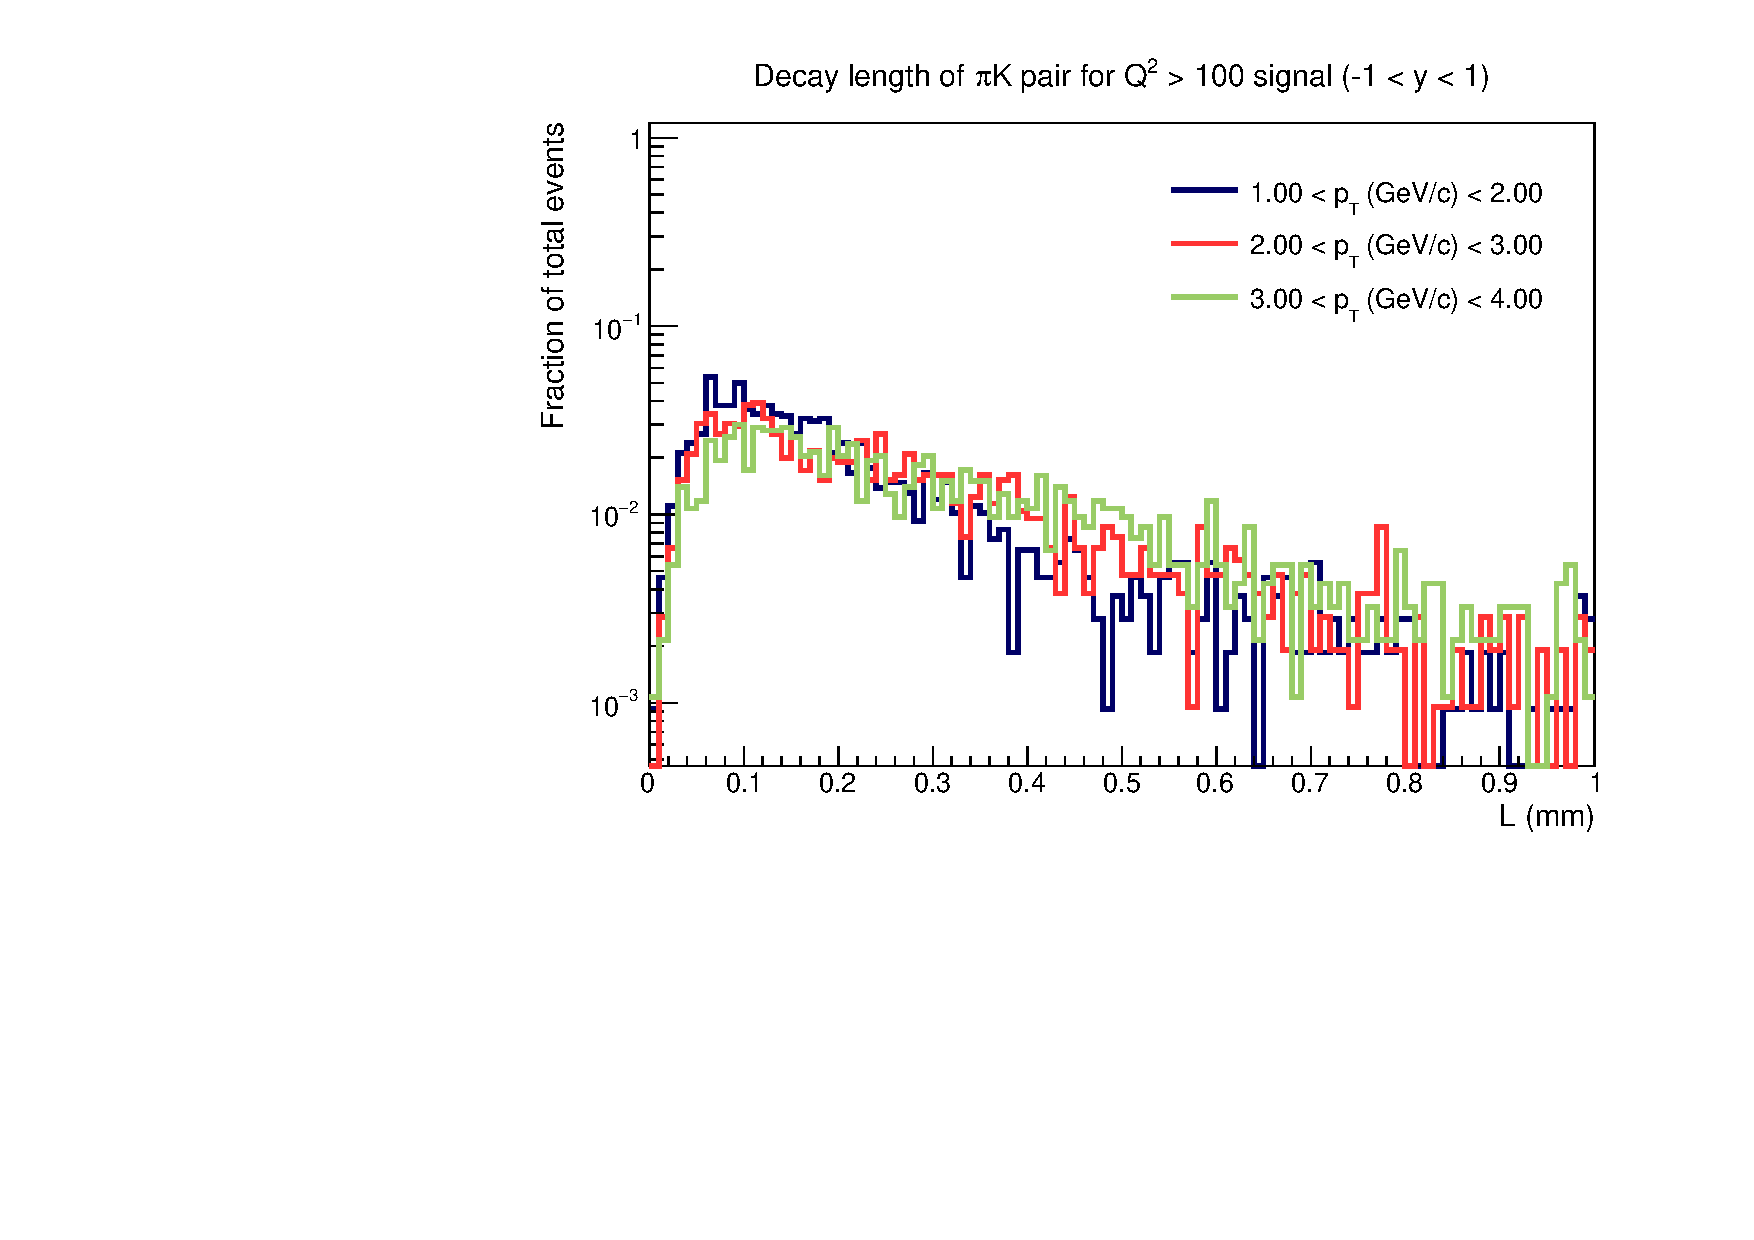
\includegraphics[width=0.55\linewidth]{gallery/D0_topology/dl_pt.pdf}
    \caption{$p_T$-dependence of the decay length of reconstructed $D^0$-mesons in simulated $Q^2>100~\text{GeV}^2$ $ep$ collisions, comparing various $p_T$ ranges for $01<y<1$.}
    \label{f.dl}
\end{figure}
%
As shown in Fig. \ref{f.dl}, the decay length exhibits the opposite dependence on $p_T$, in which the distribution seem wider at high $p_T$ (green line). This can be explained by higher-$p_T$ $D^0$-mesons traveling farther before decaying, which results in the decay length distribution peaking at a higher value.

%
\begin{figure}[h!]
    \centering
    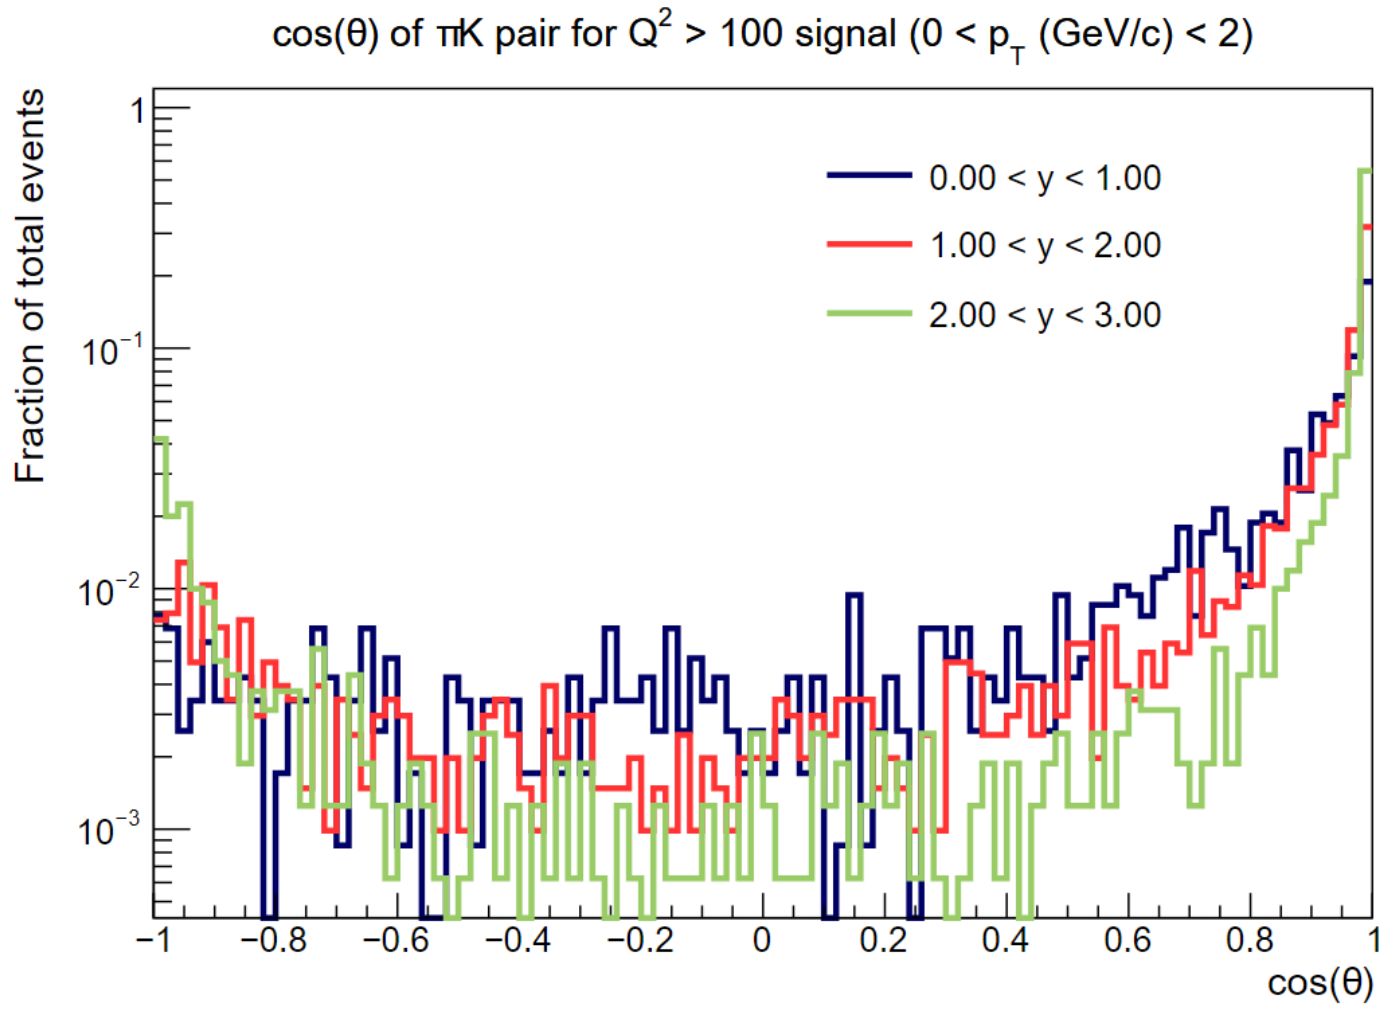
\includegraphics[width=0.55\linewidth]{gallery/D0_topology/costheta_y.png}
    \caption{$y$-dependence of $\cos{\theta}$ of reconstructed $D^0$-mesons in simulated $Q^2>100~\text{GeV}^2$ $ep$ collisions, comparing various $y$ ranges for $0<p_T<2$ GeV/c.}
    \label{f.costheta}
\end{figure}
%
When examining the topological distributions, we found that the deterioration of reconstruction performance at forward $y$ is especially apparent in plots of $\cos{\theta}$, as shown in Fig. \ref{f.costheta}. We expect the $\theta$ distribution to be centered around 0, which corresponds to the peak at $\cos{\theta}=1$. However, at forward $y$ (green line), we notice another peak at $\cos{\theta}=-1$. This second peak corresponds to $D^0$-mesons with a momentum vector $\overrightarrow{P}$ reconstructed antiparallel to its expected direction of travel, which is un-physical. This observation points toward the need for further improvements in reconstruction at forward rapidity.

% %
% \begin{figure}[hb!]
%     \centering
%     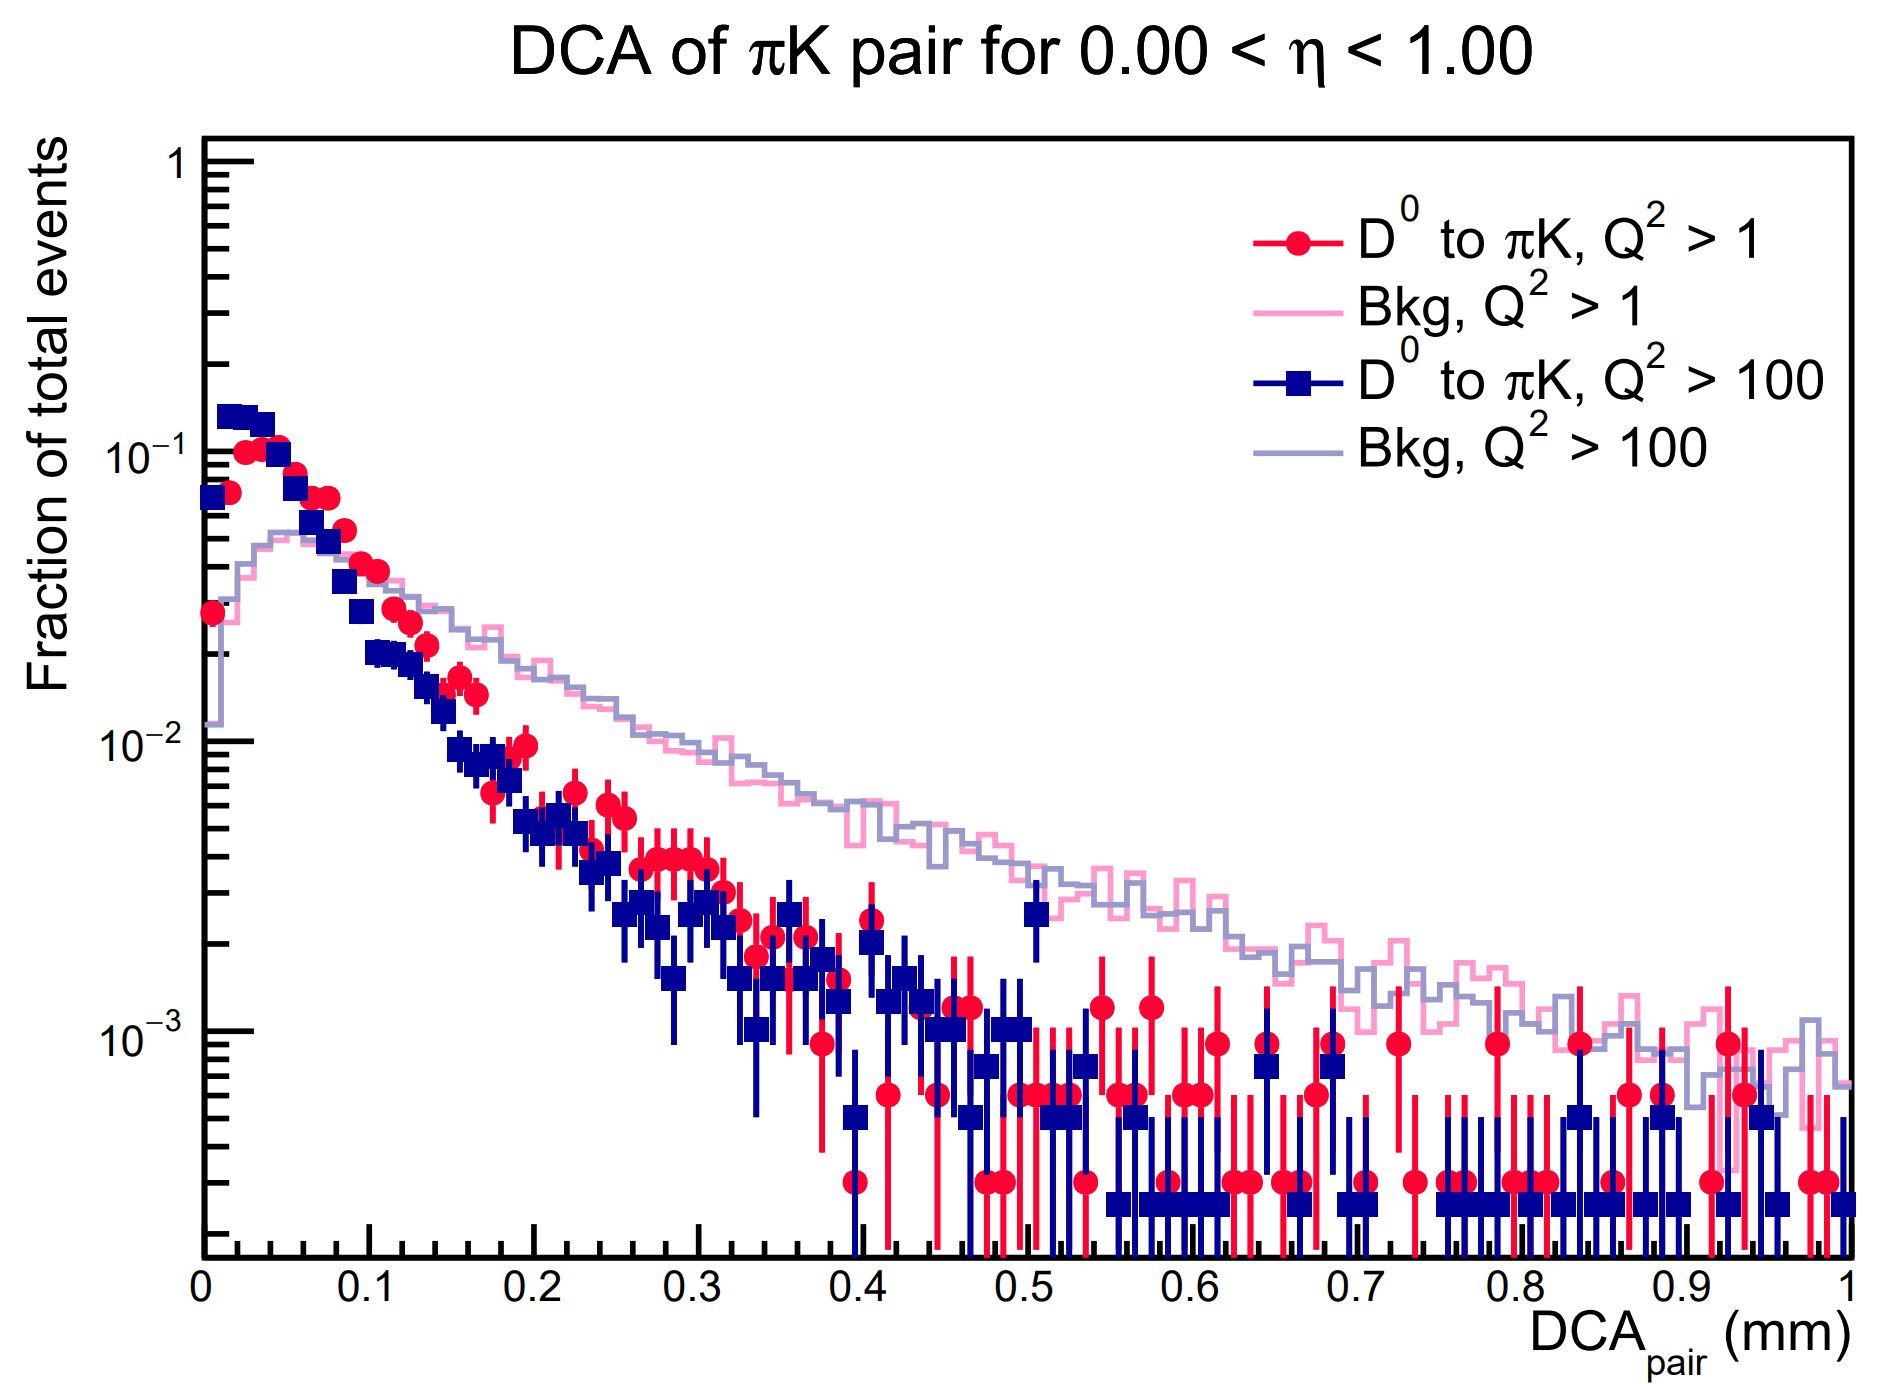
\includegraphics[width=0.45\linewidth]{gallery/D0_topology/DCA_Q2_dep.png}
%     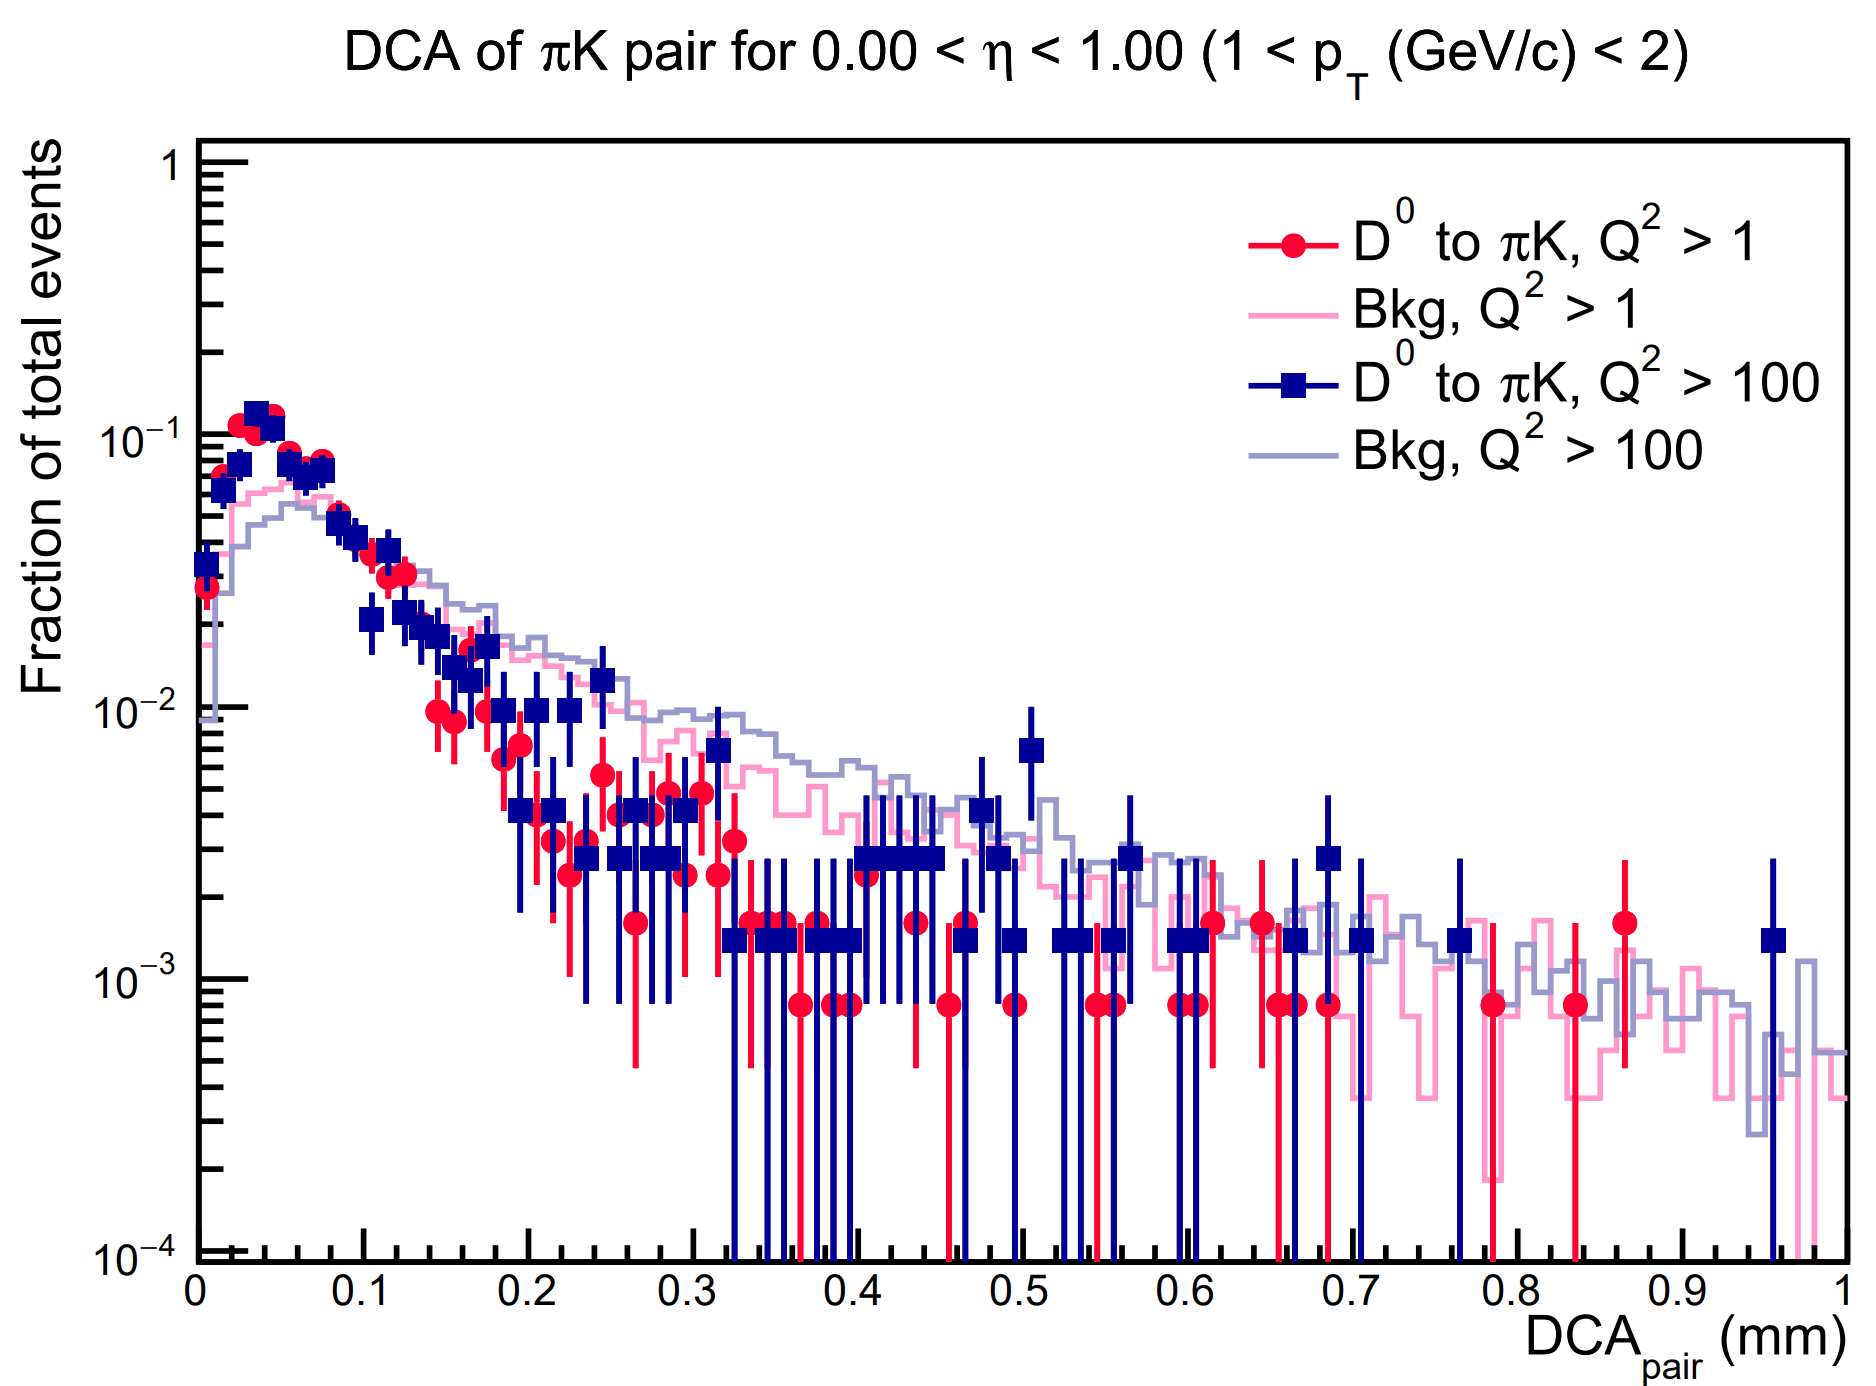
\includegraphics[width=0.45\linewidth]{gallery/D0_topology/DCA_Q2_dep_removed.png}
%     \caption{Comparison of $\text{DCA}_{D^0}$ distributions of $D^0$ signal and background candidates between $Q^2>1~\text{GeV}^2$ (red) and $Q^2>100~\text{GeV}^2$ (blue) $ep$ collisions, in the range $0<\eta<1$. The left plot shows the $p_T$-integrated distributions, and the right plot shows the distributions for the slice $1<p_T<2$.}
%     \label{f.top_by_y_pt}
% \end{figure}
% %

% %
% \begin{figure}[h!]
%     \centering
%     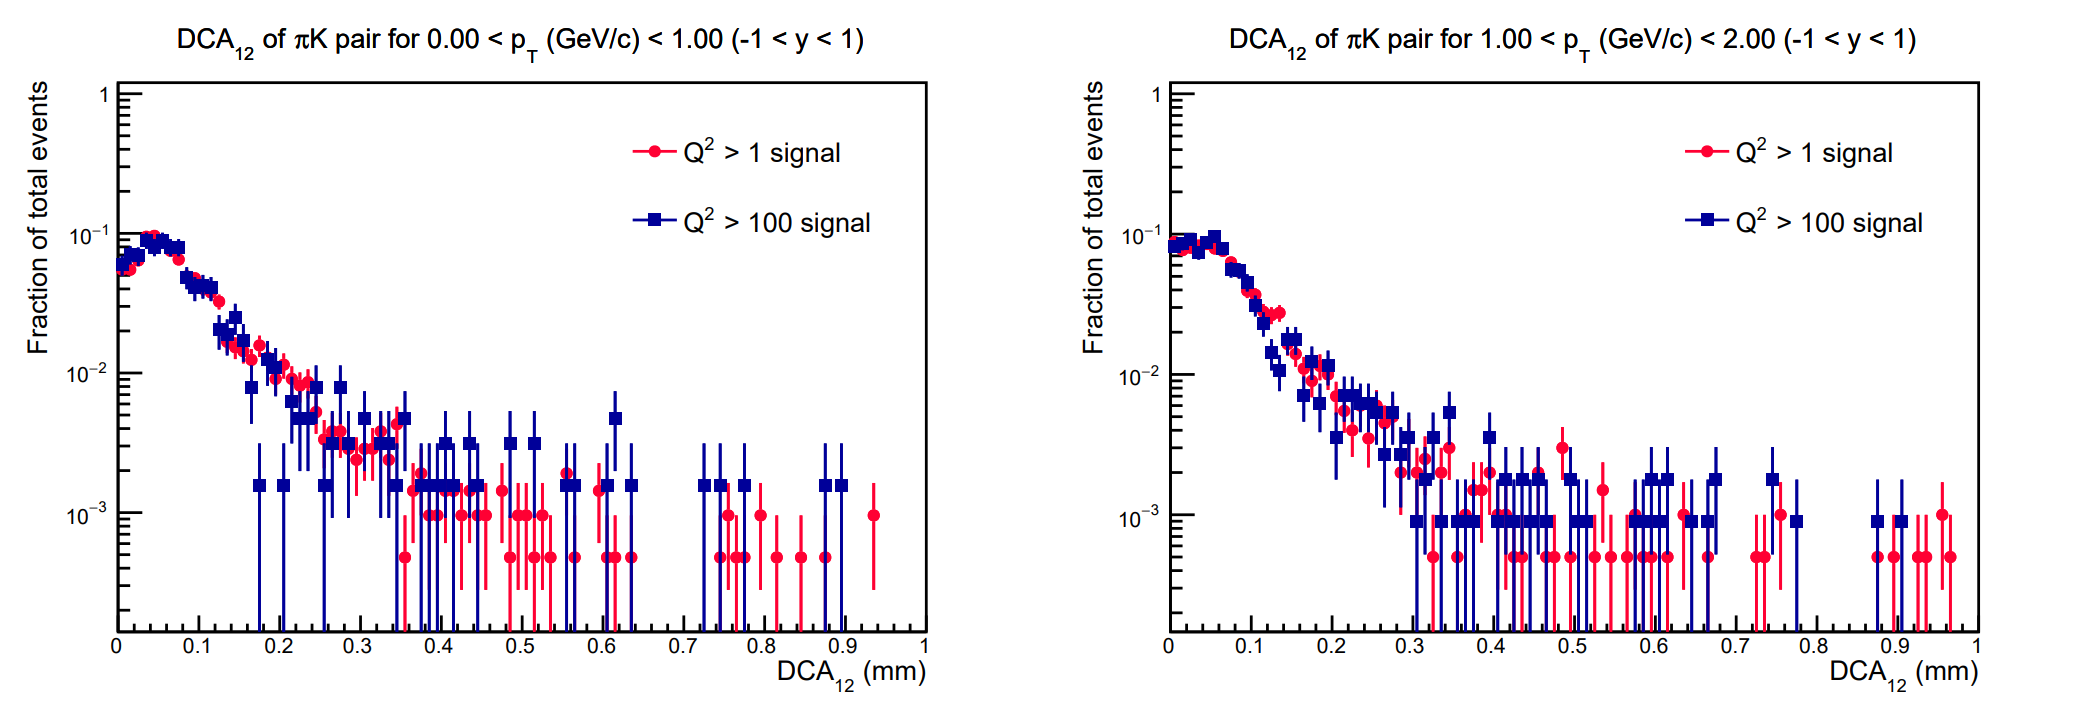
\includegraphics[width=0.95\linewidth]{gallery/D0_topology/DCA12_slices_1.png}
%     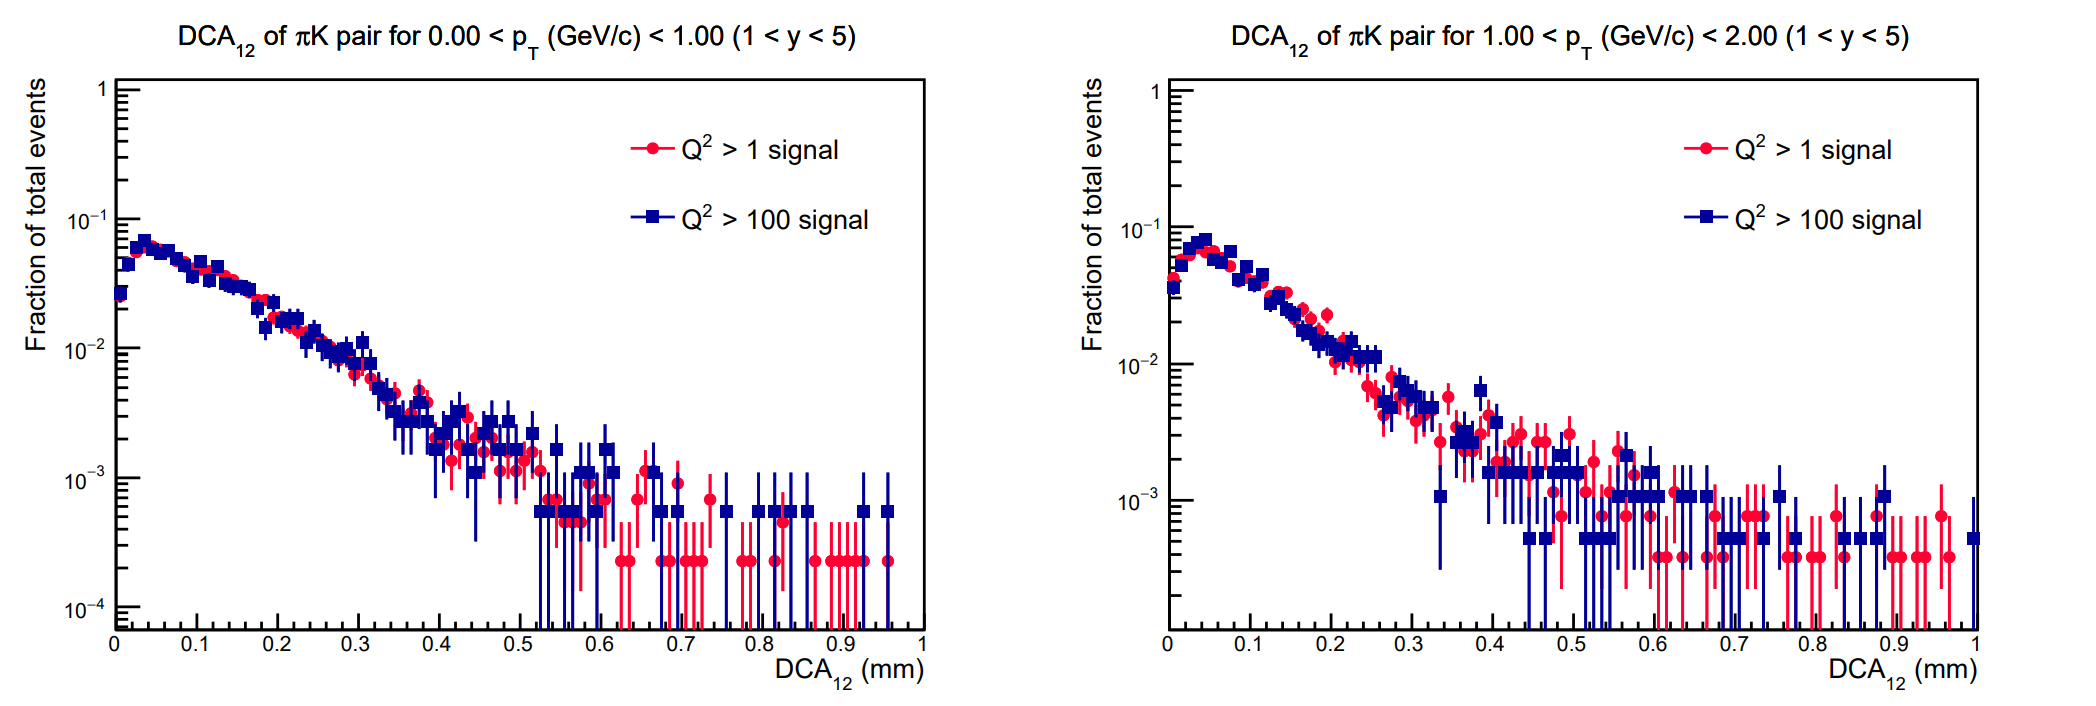
\includegraphics[width=0.95\linewidth]{gallery/D0_topology/DCA12_slices_2.png}
%     \caption{Comparison of $\text{DCA}_{12}$ distributions between $Q^2>1~\text{GeV}^2$ (red circles) and $Q^2>100~\text{GeV}^2$ (blue squares) $ep$ collisions for $D^0$ signal candidates in various slices of $y$ and $p_T$. (Can consider using a different top. var. as an example.)}
%     \label{f.top_by_Q2}
% \end{figure}
% %
%
\begin{figure}[h!]
    \centering
    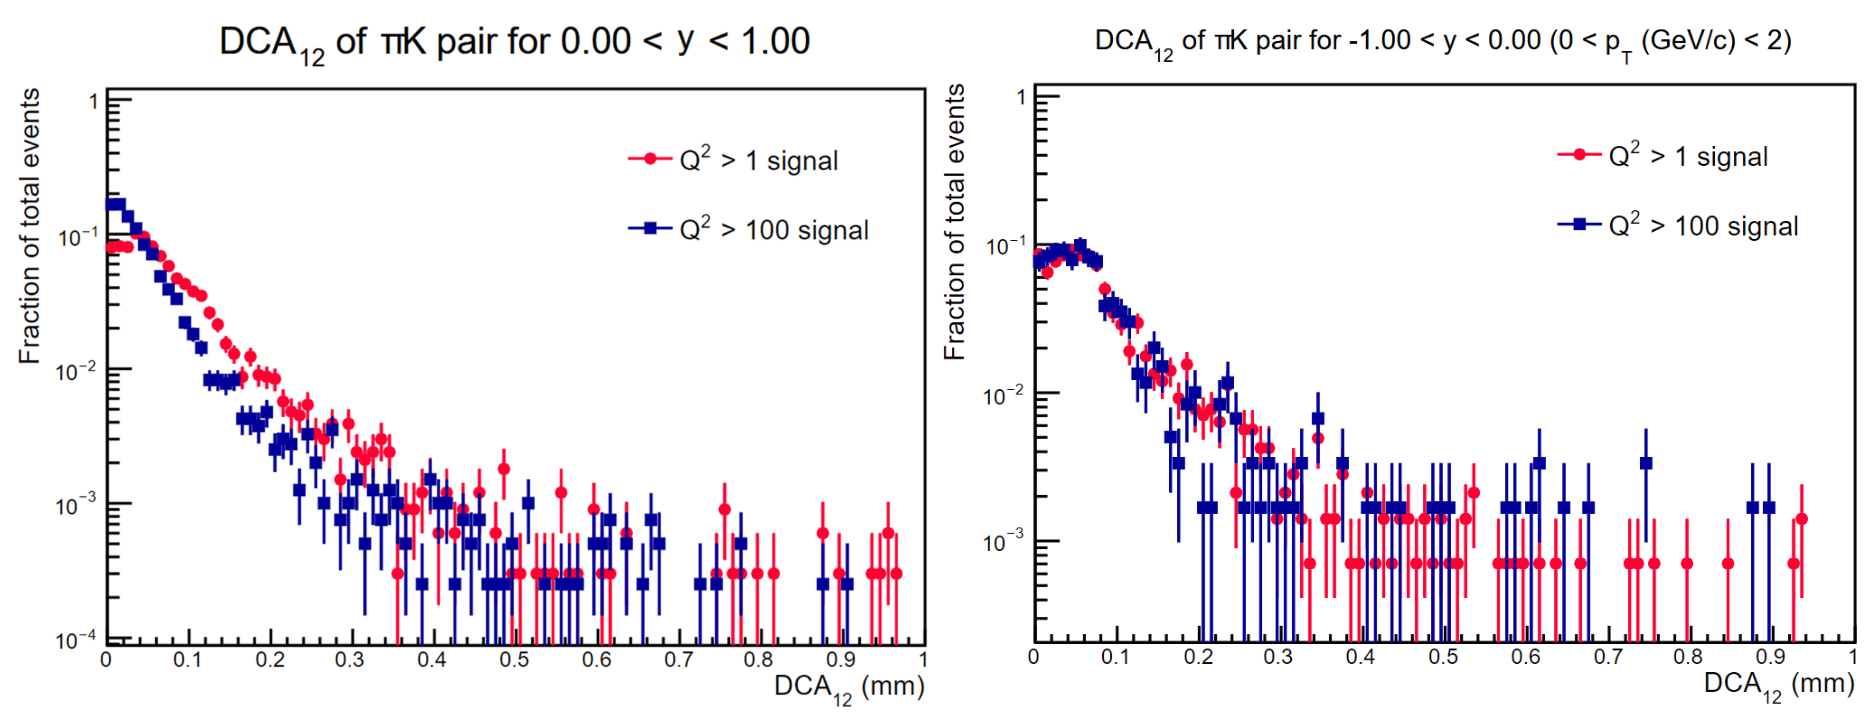
\includegraphics[width=0.9\linewidth]{gallery/D0_topology/top_q2.png}
    \caption{Comparison of $\text{DCA}_{12}$ distributions between $Q^2>1~\text{GeV}^2$ and $Q^2>100~\text{GeV}^2$$ep$ collisions for reconstructed $D^0$-mesons with any $p_T$ (left) vs. with $0<p_T<2$ GeV/c, both at mid-$y$.}
    \label{f.top_by_Q2}
\end{figure}
%
One last kinematic consideration concerns $Q^2$, defined in Ch. \ref{sec.bkg_emu}, which is the square of the four-momentum transferred in the $ep$ collision. The value of $Q^2$ determines how much energy is available for all the particles produced in the interaction. In Fig. \ref{f.top_by_y_pt}-\ref{f.costheta}, we have presented results for collisions with high four-momentum transfer, $Q^2>100~{\rm GeV^2}$. However, experiments at the EIC will also span a wide range of $Q^2$, and $ep$ collisions generally look different at various energy levels. For example, high $Q^2$ collisions tend to produce more $D^0$-mesons with large $p_T$ while low $Q^2$ collisions produce more particles with low $p_T$. Thus, we can expect the $Q^2$-dependence of topological variables to follow the same trends as their $p_T$-dependence. To examine the effects of $Q^2$ on the $D^0\rightarrow\pi+K$ topology, we compare the topological distributions of $D^0$-mesons produced in $Q^2>1~{\rm GeV^2}$ and $Q^2>100~{\rm GeV^2}$ collisions. Fig. \ref{f.top_by_Q2} shows these distributions for ${\rm DCA_{12}}$.

In the left plot, which includes all $D^0$-mesons with any $p_T$, we find that the ${\rm DCA_{12}}$ distribution is wider for $Q^2>1~{\rm GeV^2}$ collisions compared to the higher energy $Q^2>100~{\rm GeV^2}$ collisions. However, due to the correlation between $Q^2$ and $p_T$, the dependence on $Q^2$ is removed when restricting to individual $p_T$ slices. As we see in the right plot of Fig. \ref{f.top_by_Q2}, which only includes $D^0$-mesons with $0<p_T<2~{\rm GeV/c}$, there are no significant differences between the topological distributions for $Q^2>1~\text{GeV}^2$ and $Q^2>100~\text{GeV}^2$ collisions.

%--------------------------------------------------------
\section{Strategy for $D^0$ signal-background separation with topological cuts}
\label{sec.d0_strategy}

%
\begin{figure}[h!]
    \centering
    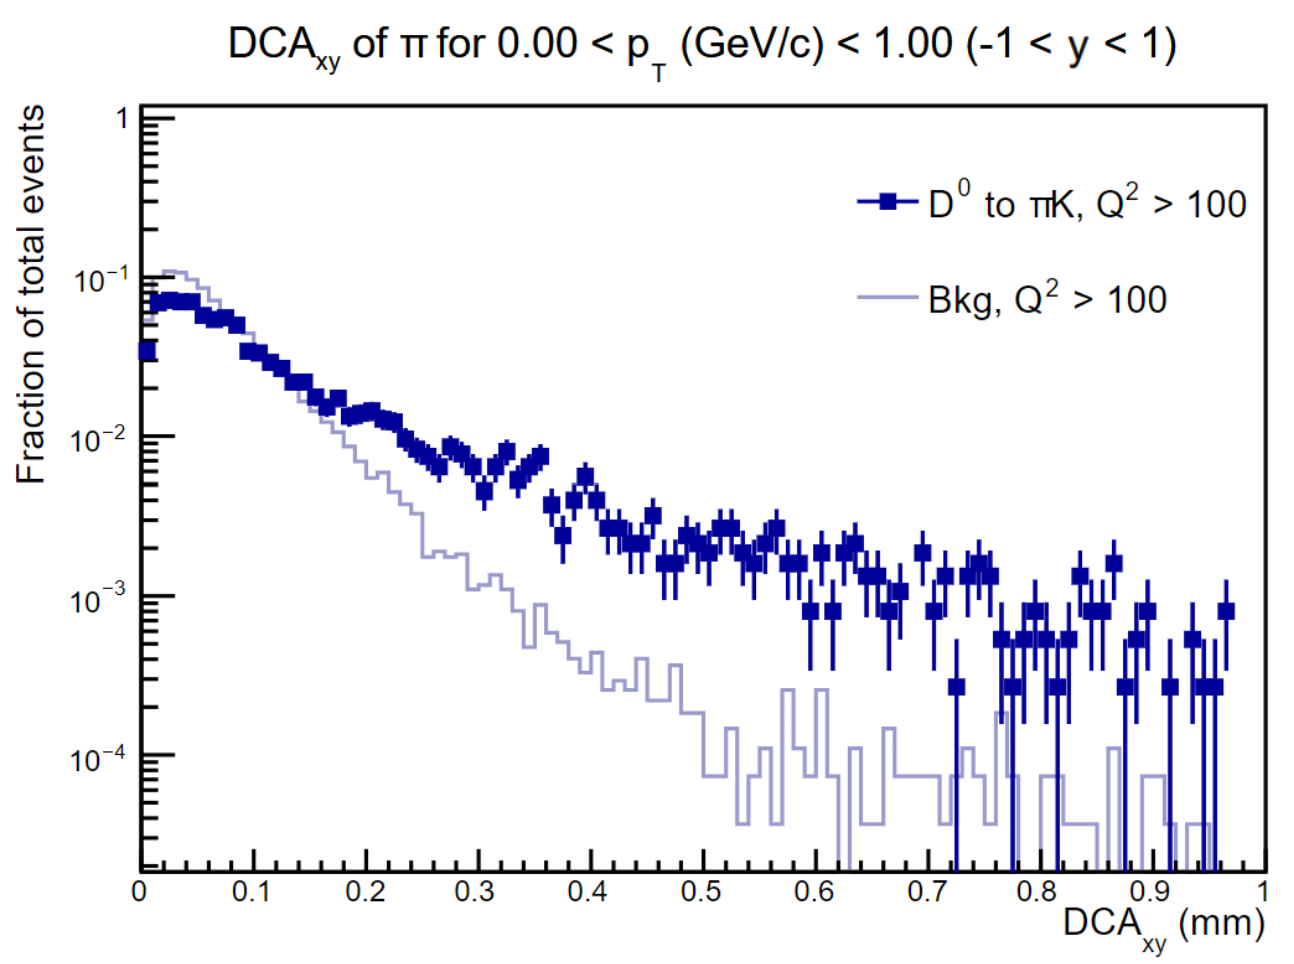
\includegraphics[width=0.6\linewidth]{gallery/D0_topology/top_cut.png}
    \caption{Example comparison of ${\text{DCA}}_{{\rm \pi}(xy)}$ distributions for reconstructed $D^0$-mesons (discrete markers) and background (line).}
    \label{f.top_cut}
\end{figure}
%
Our goal is to use the shapes of the topological distributions, which generally look different for true $D^0$-mesons (signal) and for the background. Fig. \ref{f.top_cut} shows an example comparing the signal and background distributions for ${\text{DCA}}_{{\rm \pi}(xy)}$. We would like to select some cut value $x$, such that we accept all candidates with ${\text{DCA}}_{{\rm \pi}(xy)}<x$ as signal and reject all candidates with ${\text{DCA}}_{{\rm \pi}(xy)}>x$. In practice, we will always end up accepting some mixture of signal and background candidates. However, with the help of machine learning, we can look for the most optimal cut that maximizes the number of signal candidates while minimizing the number of background candidates.

%
\begin{table}[h!]
    \centering
    \begin{tabular}{c|c|c}
                & $-1<y<1$ & $1<y<3$ \\
                \hline
    $1<p_T<2~{\rm GeV/c}$   & mid-$y$, low $p_T$ & forward $y$, low $p_T$ \\
    $2<p_T<3~{\rm GeV/c}$   & mid-$y$, high $p_T$ & forward $y$, high $p_T$ \\
    \end{tabular}
    \caption{Kinematic slices in $y$ and $p_T$ of the $D^0$ considered in this analysis.}
    \label{tab.kinematics}
\end{table}
%
In the previous section, Ch. \ref{sec.top_y_pt_slices}, we have seen that the $D^0\rightarrow\pi+K$ topology depends significantly on both $y$ and $p_T$. As a result, the set of topological cuts that gives the best signal-and-background separation for one $y$ and $p_T$ range may not perform well for other ranges. Therefore, we optimize the separation of $D^0$ signals from background for individual slices of $y$ and $p_T$. Specifically, we divide the data into the 4 kinematic categories in Table \ref{tab.kinematics}.

We do not include backward rapidity $y<-1$ and $p_T>3$ due to these regions having low statistics (see Fig. \ref{f.y_pT}), meaning that the regions are sparsely populated and thus have large statistical uncertainties. Given that we consider small slices in $p_T$. the topological distributions are independent with respect to $Q^2$. Thus, we analyze all particles for $Q^2>1~\text{GeV}^2$, which includes low and high energy collisions. In Ch. \ref{ch.results}, we will discuss the optimization of topological cuts in these various kinematic regions using machine learning.
\chapter{Machine learning methodology}
\label{ch.ml}

In this chapter, we discuss the machine learning methodology we utilize for our $D^0$ analysis. In Ch. \ref{sec.ml_bdt}, we introduce the theory of boosted decision trees (BDTs), the particular type of model used in this analysis. Then in Ch. \ref{sec.ml_implementation}, we discuss various aspects to consider when applying BDTs and interpreting the results.

% \section{Introduction to machine learning (ML)}
% \label{sec.ml_intro}

% {\color{brown}\bf Resources:}
% BDTs for high energy physics: \cite{BDT}

% \begin{itemize}
%     \item Example of fitting data
%     \item Features, output, and loss function
%     \item Gradient descent
%     \item Regression and classification
%     \item Training, validation, and application
%     \item Overfitting and underfitting
% \end{itemize}

% At its core, machine learning (ML) is about fitting data. As with any statistical analysis, our goal is to identify patterns in a given sample that can be generalized and used to make predictions on new data. 

% %-----------------------------
% \subsection{Machine learning as linear regression}

% %-----------------------------
% \subsection{Gradient descent}

% %-----------------------------
% \subsection{Types of ML models}

% %-----------------------------
% \subsection{Training, validation, and application}

%--------------------------------------------------------
\section{The boosted decision tree (BDT) model}
\label{sec.ml_bdt}


%-----------------------------
\subsection{Decision tree classifiers}

\begin{figure}[h!]
    \centering
    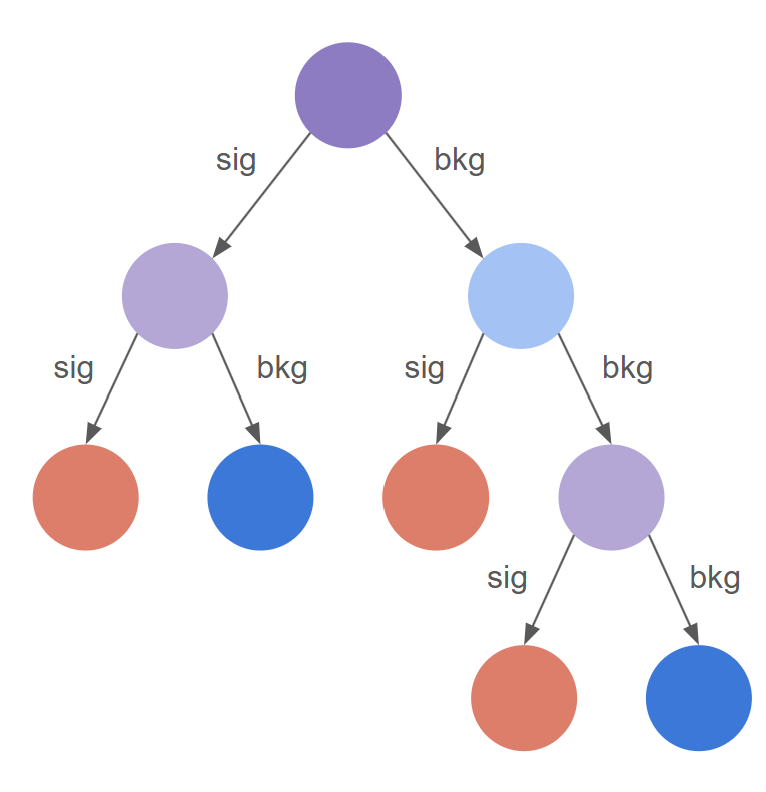
\includegraphics[width=0.4\linewidth]{gallery/ML/decision_tree.png}
    \caption{A decision tree model.}
    \label{f.decision_tree}
\end{figure}
%

A decision tree is a type of machine learning model that classifies data into discrete categories (or classes) by iteratively applying selections on the data features. In this analysis, the data consists of all the reconstructed $D^0$ and background candidates, and the two classes are $D^0$ signal and background. (This is a {\it binary} classification problem, which only involves two classes. In general, decision trees can also be used to separate data into three or more classes.) The features of the data are the topological variables discussed in Ch. \ref{sec:def_top_vars}.

Fig. \ref{f.decision_tree} provides a schematic of a decision tree model. All of the data starts in the top node, known as the root node. The algorithm tries to separate the data into signal and background classes by testing cuts on every possible topological variable, then selects the optimal cut which results in the cleanest separation. According to this topological cut, the data is split into two subsequent child nodes. At each subsequent node, the algorithm repeats the same steps to continue separating the data. When some termination condition is achieved at a given node, that node is prevented from splitting and becomes a leaf node. Common termination conditions include reaching a minimum number of candidates (node size), or achieving a minimum or maximum purity $p$, a value that represents the percentage of signal or background candidates in the node \cite{BDT}. Through this process, the decision tree learns the shape of the multi-dimensional boundaries between signal and background candidates, with respect to the topological features.

When the tree stops splitting, training of the model is complete. In the end, every candidate will have been sorted into one of the signal or background leaf nodes. Each candidate is assigned a prediction, a value representing the likelihood of the candidate being a true signal or background. Depending on the model implementation, this prediction can be a continuous quantity, such as a probability, or a discrete value, such as +1 for belonging to a signal leaf node and 0 (or -1) for belonging to a background leaf node.

Decision trees are structurally simple and functionally intuitive, making them a desirable tool for solving optimization problems in physics. However, they are prone to overfitting and are often unstable, meaning that small changes in the training data can dramatically alter the model structure \cite{BDT}. To offer some insight into this issue, consider the following hypothetical. In order to achieve the cleanest separation of signal and background data, we will most likely want the tree to continue growing until the nodes achieve a very high purity. This will result in a deep tree with many splittings. However, by attempting to perfectly classify all events, the tree becomes sensitive to outliers and noise in the data, memorizing details that are unique to the training data rather than learning general patterns. On the other hand, adopting weak purity requirements to constrain the tree depth can also limit the model's ability to discriminate between signal and background data, still resulting in poor performance.

This is an illustration of the {\it bias-variance tradeoff} in machine learning, in which reducing the rate of incorrect model output (bias) tends to increase model sensitivity to fluctuations in the training data (variance) \cite{BDT}. Often, high bias leads to underfitting while high variance leads to overfitting. Increasing complexity, such as by increasing the depth of a decision tree, tends to tip the model toward high variance. The challenge then is to balance bias and variance in order to both achieve high discriminative ability and mitigate the tendency of overfitting. This is where {\it boosting} comes in.

%-----------------------------
\subsection{Gradient boosting}
\label{sec.ml_gradient_boosting}

%
\begin{figure}[h!]
    \centering
    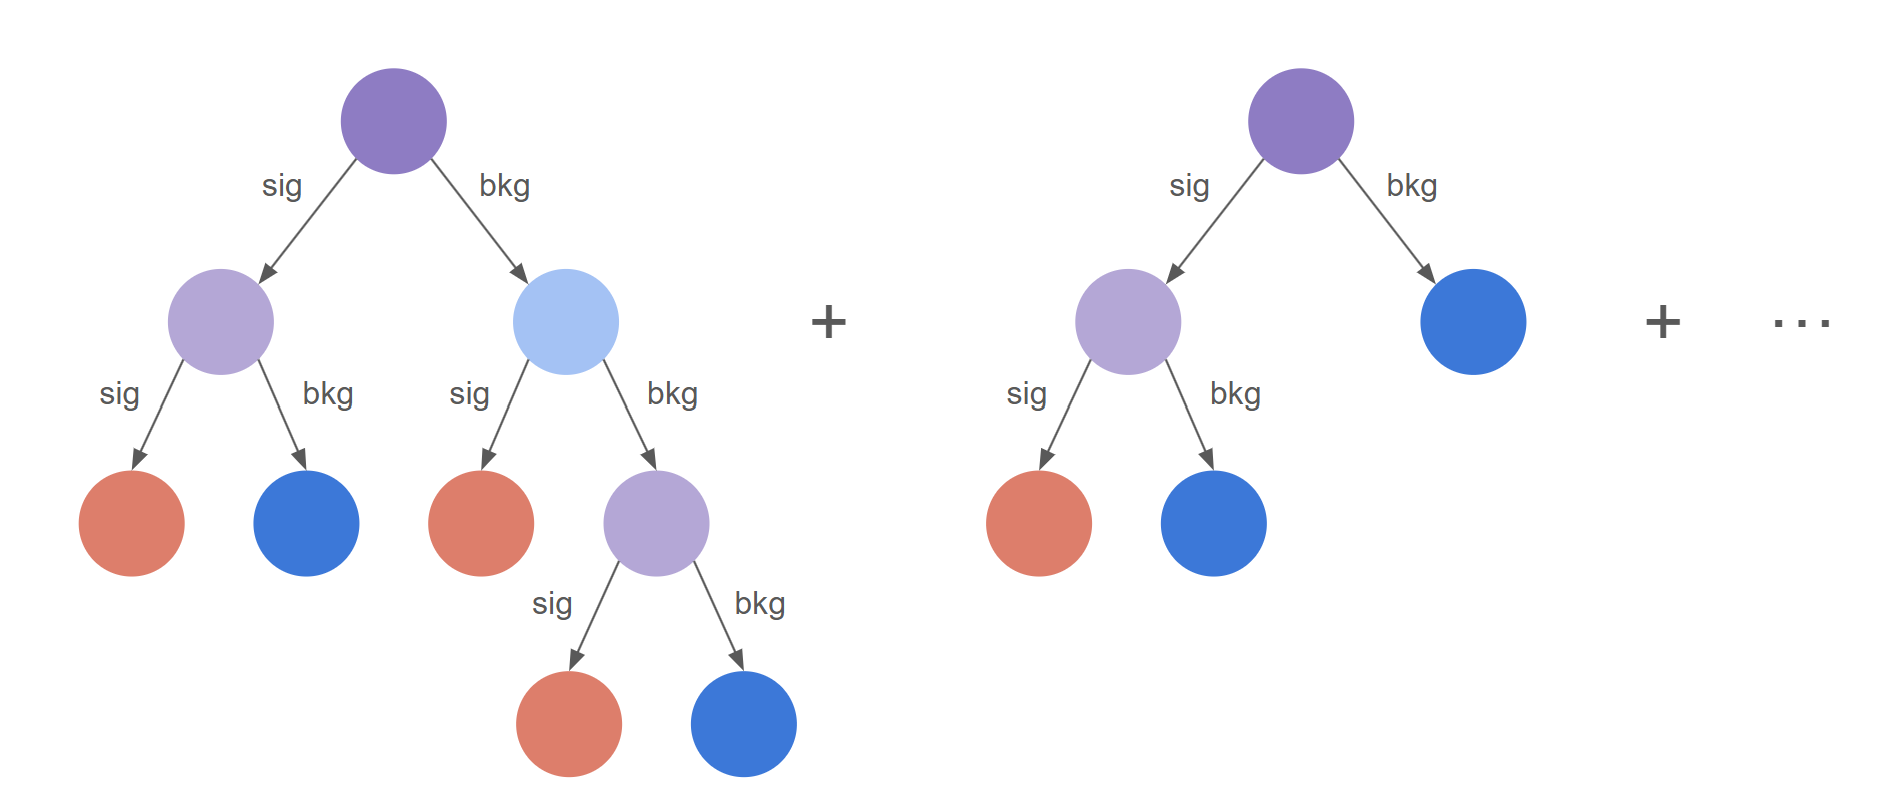
\includegraphics[width=0.9\linewidth]{gallery/ML/boosted_decision_tree.png}
    \caption{A boosted decision tree model.}
    \label{f.boosted_decision_tree}
\end{figure}
%
Boosting is a form of {\it ensemble learning}, meaning that the final ML output is an ``average" of results obtained from a collection (or ensemble) of many individual models, called {\it base learners}. In a boosted decision tree (BDT), the base learners are shallow trees, each with weak discriminative ability. Collectively, the entire ensemble is able to achieve much greater discriminative ability than any one individual tree, and limiting the complexity of each tree also leads to less variance. This analysis employs the particular method of gradient boosting \cite{friedman}, implemented through the eXtreme Gradient Boosting (XGBoost) system \cite{XGBoost}. Below, we present the general framework of a gradient-boosted decision tree.

Consider a dataset with $n$ candidates and $m$ features, $\mathcal{D} = \{(\mathbf{x}_i,y_i) \}$ for $i=1,2,...,n$, where the $i$-th candidate is represented by the data point $(\mathbf{x}_i,y_i)$. The input is a vector $\mathbf{x}_i = (x_i^{(1)},~x_i^{(2)},~...~,x_i^{(m)}) \in \mathbb{R}^m$, where the component $x_i^j$, for $j=1,2,...,m$, represents the value of feature $j$ for candidate $i$. The true output is a number $y_i \in \mathbb{R}$, where $y_i=0$ if the candidate is background and $y_i=1$ if the candidate is signal.

Let the BDT model $\mathcal{F}$ consist of $T$ trees, each represented mathematically by some function $f^{(t)}$, where $t=1,2,...,T$ labels the tree number. The model is built additively, incorporating an additional tree at each step of the gradient boosting \cite{friedman}.
\begin{equation}
    \mathcal{F} = \mathcal{F}^{(0)} + \sum_{t=1}^T f^{(t)} \ ,
    \label{eqn.model}
\end{equation}
where $\mathcal{F}^{(0)}$ is some initial guess model. The final model prediction for each candidate is the simple sum of individual predictions obtained from all $T$ trees. Note that the base learner trees are not independent; rather, the predictions given by each tree depends on the results of the previous tree. We will discuss the interpretation of these results in more detail at the end of this section. First, let us address how the BDT model is trained.

At the $t$-th step in the boosting algorithm, the predicted output for candidate $i$ is \cite{friedman}
\begin{equation}
    \hat{y}_i^{(t)} \equiv \mathcal{F}^{(t)}(\mathbf{x}_i) = \mathcal{F}^{(0)}(\mathbf{x}_i) + \sum_{t'=1}^t f^{(t')}(\mathbf{x}_i) \ ,
    \label{eqn.yhat}
\end{equation}
where $\mathcal{F}^{(t)}$ is the state of the BDT model at this step.  We can rewrite Eq. \eqref{eqn.yhat} in the iterative form
\begin{equation}
    \hat{y}^{(t)}_i = \hat{y}^{(t-1)}_i + f^{(t)}(\mathbf{x}_i) \ .
    \label{eqn.yhat2}
\end{equation}

Like all machine learning models, BDTs optimize the classification of data by minimizing the {\it loss function} over all $n$ data points, which represents the distance between the model predictions and the true outputs. At the $t$-th step, the total loss function is \cite{friedman}
\begin{equation}
    \mathcal{L}[\mathcal{F}^{(t)}] = \sum_{i=1}^n L \left[y_i, \hat{y}^{(t)}_i \right] = \sum_{i=1}^n L \left[y_i, \hat{y}^{(t-1)}_i+f^{(t)}(\mathbf{x}_i) \right] \ ,
\end{equation}
where $L$ is some base learner loss function.

As the name suggests, gradient boosting uses a {\it gradient descent} algorithm to find the minimum of the loss function. At the $t$-th step, the gradient vector is $\mathbf{\nabla}\mathcal{L}^{(t)} \in \mathbb{R}^n$ \ , where the $i$-th component is
\begin{equation}
    \mathbf{\nabla}\mathcal{L}_i^{(t)} = \frac{\partial L[y_i, \hat{y}^{(t-1)}_i ]}{\partial \hat{y}^{(t-1)}_i} \ ,
\end{equation}
with $\hat{y}^{(t-1)}_i$ given by Eq. \eqref{eqn.yhat2}. Thus, to minimize the total loss $\mathcal{L}$, the function $f^{(t)}$ for tree $t$ is chosen to approximate the target $\tilde{f}^{(t)} \equiv -\mathbf{\nabla}\mathcal{L}^{(t)}$, also known as the {\it pseudo-residual}. This means that the prediction $\hat{y}^{(t)}_i$ of each tree must be a continuous variable, rather than a discrete label for signal or background.

To offer a more intuitive understanding of what the pseudo-residual is and what each decision tree actually contributes to the final BDT prediction, consider a base learner loss function given by the mean squared error (MSE) \cite{gradient_boosting},
\begin{equation}
    L[y_i, \hat{y}^{(t)}_i] = \frac{1}{2}(y_i- \hat{y}^{(t)}_i )^2 \ .
\end{equation}
For this loss function, the $i$-th component of the gradient is
\begin{equation}
    \mathbf{\nabla}\mathcal{L}_i^{(t)} = -(y_i- \hat{y}^{(t-1)}_i) = - \tilde{f}^{(t)}(\mathbf{x}_i) \ .
\end{equation}
Here, the target function $\tilde{f}^{(t)}$ for step $t$ is precisely the residual between the true value and the prediction obtained from the previous step. Now looking back at the BDT model $\mathcal{F}$ in Eq. \eqref{eqn.model}, we can understand the result of each tree to be a marginal prediction, and we can then think of the next tree as being trained on the remaining residual. Generalizing to other types of loss functions, we can similarly interpret $f^{(t)}$ to be the function for tree $t$ that best reduces the distance between the true values and previous model predictions. With each boosting step, the model predictions inch closer to the true values.

In practice, rather than adding all the marginal contributions of each tree in a simple sum as in Eq. \ref{eqn.model}, we weight each contribution by a small number $\eta$, called the {\it learning rate}. The overall BDT model is then \cite{friedman}
\begin{equation}
     \mathcal{F} = \mathcal{F}^{(0)} + \eta \sum_{t=1}^T f^{(t)} \ . \label{eqn.model_eta}
\end{equation}
The learning rate determines the size of each boosting step, whose value is set so that the model descends smoothly toward the minimum of the loss function $\mathcal{L}$.

%---------------------------------------------------------
\section{BDT implementation}
\label{sec.ml_implementation}
For this thesis, we use the XGBoost \cite{XGBoost} library, a framework that implements gradient-boosted decision trees, which is handled through the Minimal heavy ion physics environment for Machine Learning (hipe4ml) Python library \cite{hipe4ml}. In this section, we discuss the practical application of BDTs in our $D^0$ analysis, focusing on the tools we use to assess BDT performance (Ch. \ref{sec.ml_performance}), determine feature importance (Ch. \ref{sec.ml_shap}), and adjust hyperparameters (Ch. \ref{sec.ml_optuna}).

%-------------------------
\subsection{BDT training and performance}
\label{sec.ml_performance}

We combine all the reconstructed $D^0$ signal and background candidates into a dataset $\mathcal{D}=\{(\mathbf{x}_1,y_1), (\mathbf{x}_2,y_2),\dots,(\mathbf{x}_n,y_n) \}$, with each $\mathbf{x}_i\in\mathbb{R}^m$. This represents our $n$ total candidates (or data points) with $m$ topological features. The true output values are $y_i=0$ for background candidates and $y_i=1$ for signal candidates. To avoid introducing bias, we include an equal number of true signal and background candidates in $\mathcal{D}$. We randomly split the data into a training set $\mathcal{D}_{\rm train}$, which is used to train the BDT, and a testing set $\mathcal{D}_{\rm test}$, which is used to test the trained model on ``new" data. We adopt a typical split of $80\%$ training data and $20\%$ testing data.

For each candidate, the BDT returns a predicted output ($\hat{y}$), a value between $0$ and $1$, which represents the confidence with which the BDT believes the candidate is a true signal. A BDT output close to $1$ indicates the candidate is most likely signal, and a score close to $0$ indicates the candidate is most likely background. Fig. \ref{f.ml_bdt_score} shows an example distribution of BDT outputs assigned to candidates in the training dataset (filled histograms) vs. the testing dataset (solid markers). In red we have the signal candidates, whose distributions peak near $1$, and in blue we have the background candidates, whose distributions peak near $0$. 

%
\begin{figure}[h!]
    \centering
    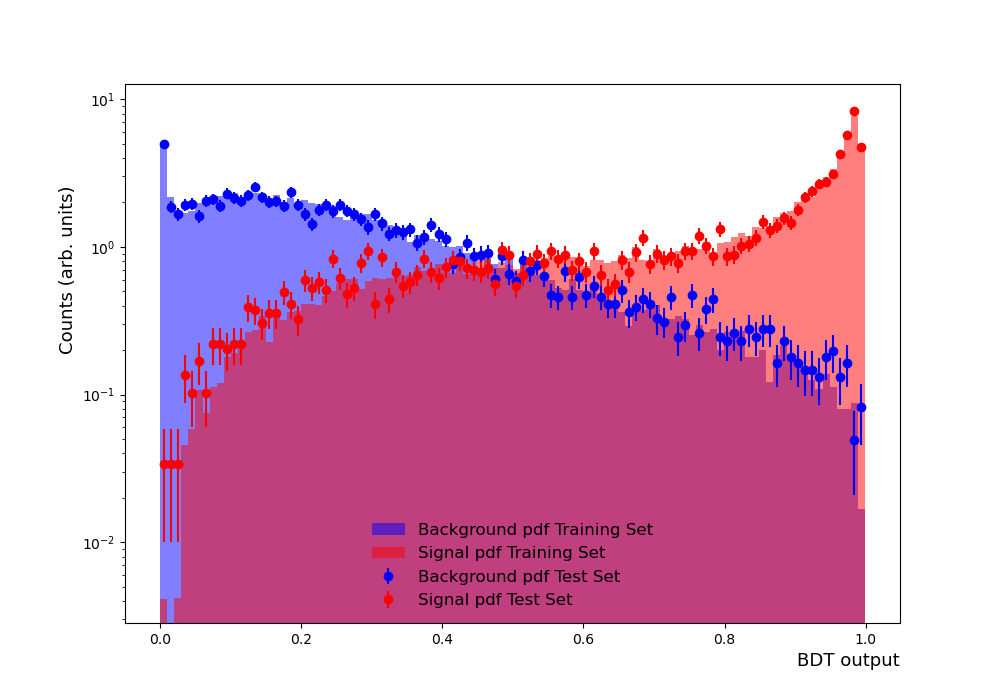
\includegraphics[width=0.6\linewidth]{gallery/results/train_test_without_bkg.png}
    \caption{Example of BDT outputs for training vs. test data. Training data are plotted as shaded histograms and test data are plotted as solid markers, with true background candidates in blue and true signal candidates in red}
    \label{f.ml_bdt_score}
\end{figure}
%
Here, we have essentially distilled all the features of the data into a single variable. Rather than applying cuts by hand on all $m$ features to find the optimal signal-and-background separation (as we would normally do without machine learning), we now only need to apply a one-dimensional cut on the BDT output. When we apply the trained BDT to analyze new data, the model will provide a BDT output for each candidate. We would then choose a BDT threshold value, perhaps $0.5$ for example, then accept all candidates with BDT output $>0.5$ as signal and reject those with BDT output $<0.5$ as background. 

In practice, there often is not a clean separation between the signal and background distributions, as is the case in Fig. \ref{f.ml_bdt_score}, because some features of signal and background candidates can look similar to each other. Due to this overlap, we select the BDT score threshold that best optimizes some metric of interest. In our analyses, the quantity we optimize to is the {\it significance} \cite{BDT},
\begin{equation}
    {\rm Signif} = \frac{N_{\rm sig}}{\sqrt{N_{\rm sig}+N_{\rm bkg}}} \ , \label{eqn.signif}
\end{equation}
where $N_{\rm sig}$ is the number of true signal candidates accepted, $N_{\rm bkg}$ is the number of true background candidates accepted, and $\sqrt{N_{\rm sig}+N_{\rm bkg}}$ represents the statistical uncertainty. Another quantity of interest that represents the effectiveness of classification is the {\it signal-to-background ratio},
\begin{equation}
    {\rm S/B} = \frac{N_{\rm sig}}{N_{\rm bkg}} \ .\label{eqn.s_over_b}
\end{equation}

Another important question to examine in these plots is how much the outputs for training and testing data differ. In the example in Fig. \ref{f.ml_bdt_score}, we observe that the distributions for training data (shaded histograms) and testing data (solid markers) follow each other closely, which means that the BDT outputs are consistent across both datasets. This indicates that the BDT is well-trained and stable. On the other hand, large discrepancies between the training and testing distributions would be a sign of overtraining.

%
\begin{figure}[h!]
    \centering
    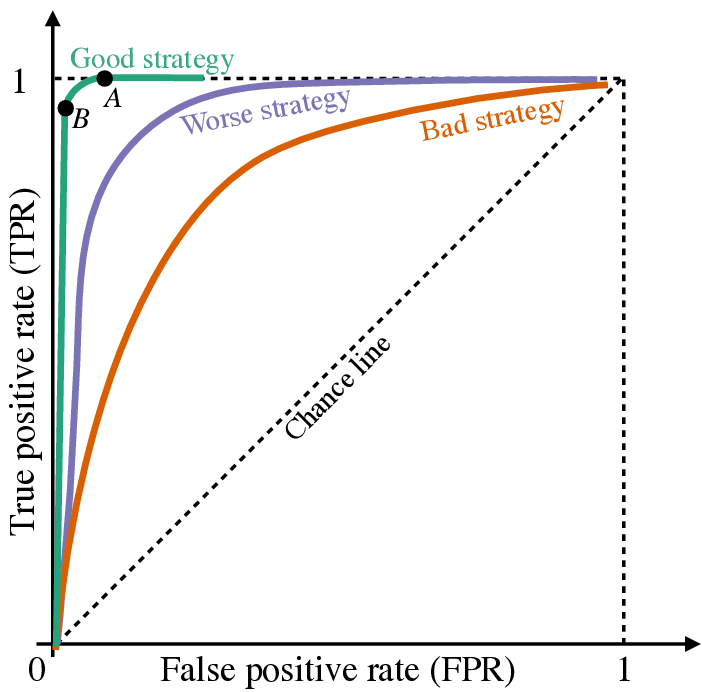
\includegraphics[width=0.5\linewidth]{gallery/ML/roc_ex.png}
    \caption{Examples of receiver operating characteristic (ROC) curves for models with varying levels of performance. Figure from \cite{roc_ex}.}
    \label{f.ml_roc}
\end{figure}
%
Complementary to plots of BDT output, we also examine the {\it receiver operating characteristic} (ROC), shown in Fig. \ref{f.ml_roc}, which illustrates the overall accuracy of the model. On the $y$-axis is the true positive rate (TPR), the fraction of true signal candidates that the model correctly classifies as signal. On the $x$-axis is the false positive rate (FPR), the fraction of true background candidates that the model misclassifies as signal. The ROC curve is produced by calculating the TPR and FPR for various possible threshold values of the BDT output \cite{BDT}, such that each point on the curve represents the result for a different threshold. In this way, the ROC curve summarizes the BDT output distributions of Fig. \ref{f.ml_bdt_score}. (We can separately produce a ROC curve for the testing and training data, which should be very similar to each other for a well-trained model.)

The green ``good strategy" curve in Fig. \ref{f.ml_roc} very closely approximates an ideal model, with a TPR that approaches $1$ very quickly. The dashed ``chance line" denotes the ROC curve resulting from random chance, with the TPR always equal to the FPR. In general, the ROC curve of a properly trained model should be between the good strategy curve and the chance curve, with curves closer to the chance line indicating worse performance. We can also measure the performance more quantitatively by integrating the area under the curve (AUC) from $0$ to $1$ along the $x$-axis. An ideal model would yield ${\rm AUC}=1$, the chance line would yield ${\rm AUC}=0.5$, and as a rule of thumb, a good model should yield ${\rm AUC}>0.8$. 


%-------------------------
\subsection{Examining feature importance with SHAP}
\label{sec.ml_shap}

When using BDTs to analyze data, the choice of features can impact the discriminative ability of the model. Features for which the signal and background distributions look very different will generally provide better discriminative ability than features for which the signal and background are similar. During training, the more discriminative features will have a greater impact on the structure of the BDT.

A method of understanding the relative importance of features used to train a machine learning model is by examining their SHAP values \cite{SHAP}. The SHapley Additive exPlanations (SHAP) tool calculates the marginal contributions of each feature by considering how often a given feature is used during training, and how much each instance of the feature use improves the overall model performance. For BDTs, the SHAP value for each feature is determined by the number nodes in which that feature is used to split the data, as well as the increase in purity resulting from each of those splits.

%
\begin{figure}[h!]
    \centering
    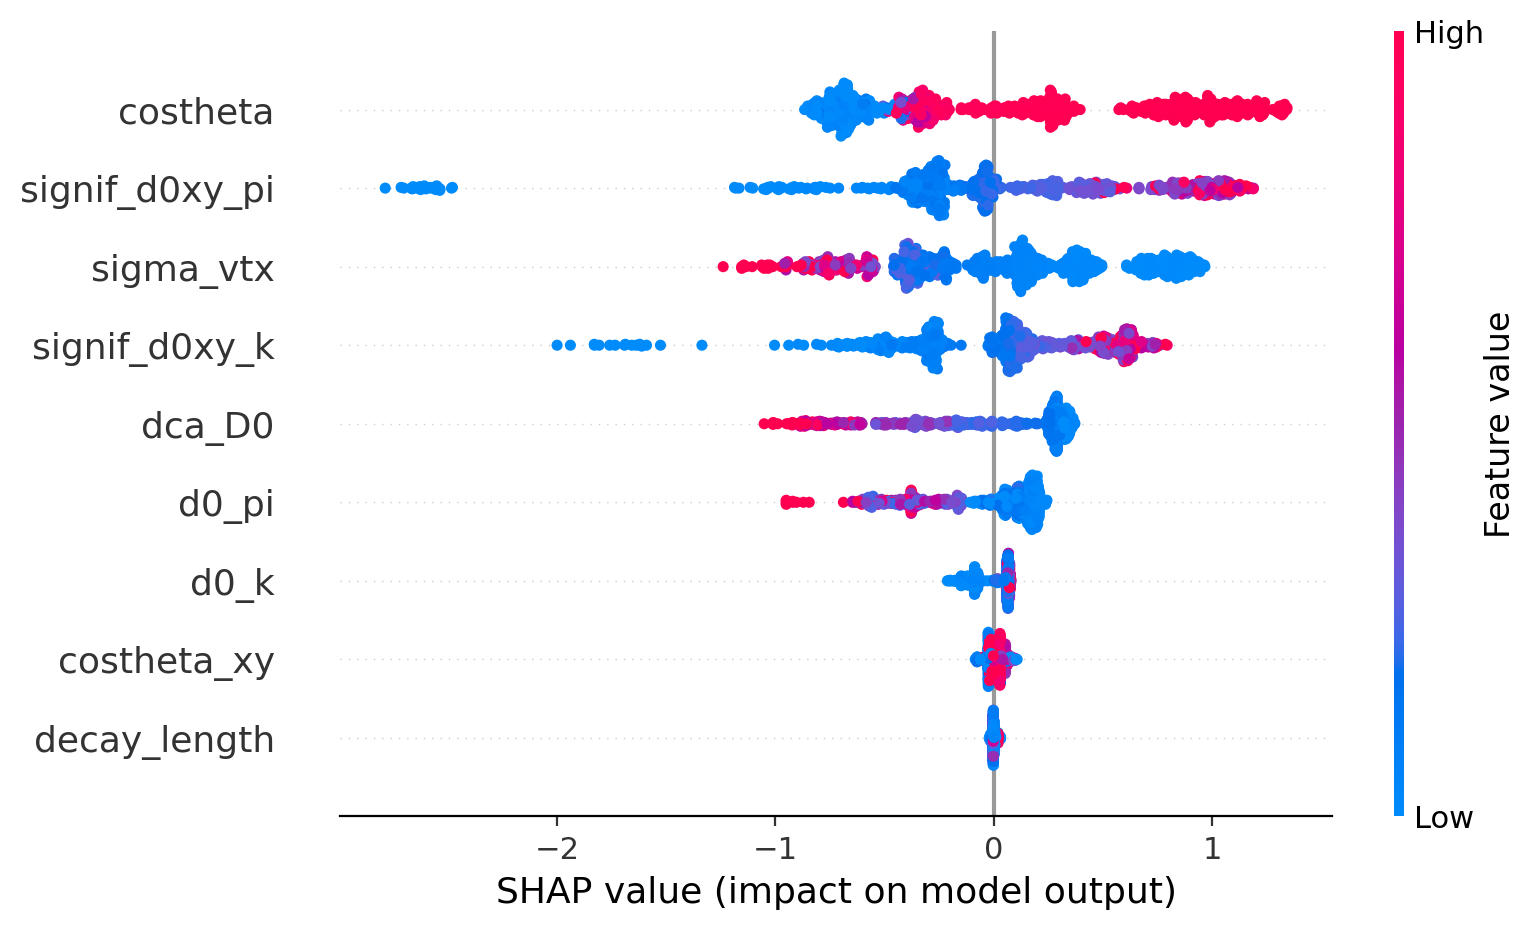
\includegraphics[width=0.95\linewidth]{gallery/ML/ex_shap_beeswarm.png}
    \caption{Example beeswarm plot of SHAP values for topological features used to train a BDT.}
    \label{f.ml_beeswarm}
\end{figure}
%
Fig. \ref{f.ml_beeswarm} shows an example ``beeswarm" plot of the SHAP values for features used to train a particular BDT model. Each point in the plot represents one candidate. Positive SHAP values indicate features that ``push" the BDT output of that candidate toward 1 (signal), and negative SHAP values indicate features that ``push" the BDT output toward 0 (background), with larger absolute values indicating higher impact. The color of each point represents the value of the topological feature for that candidate. The features are organized in order of importance, with the top feature (\texttt{costheta}) being most important. We can see the feature importance reflected in the separation of high value and low value points in the plot. More important features exhibit a more distinct separation of colors, which suggests that these features provide greater discriminative ability.

For example, looking at the \texttt{costheta} feature, we observe that high values of $\cos{\theta}$ (pink) tend to push the BDT outputs of candidates toward 1 while low values tend to push the BDT output toward 0. We can interpret this to mean that candidates with higher (more positive) values of $\cos{\theta}$ are more likely to be signal, and candidates with lower (more negative) values of $\cos{\theta}$ are more likely to be background. If we now look at \texttt{decay\_length}, we observe that neither high and nor low features values push the BDT outputs in a particular direction, so this feature is not very useful in determining whether a given candidate is signal or background.

%
\begin{figure}[h!]
    \centering
    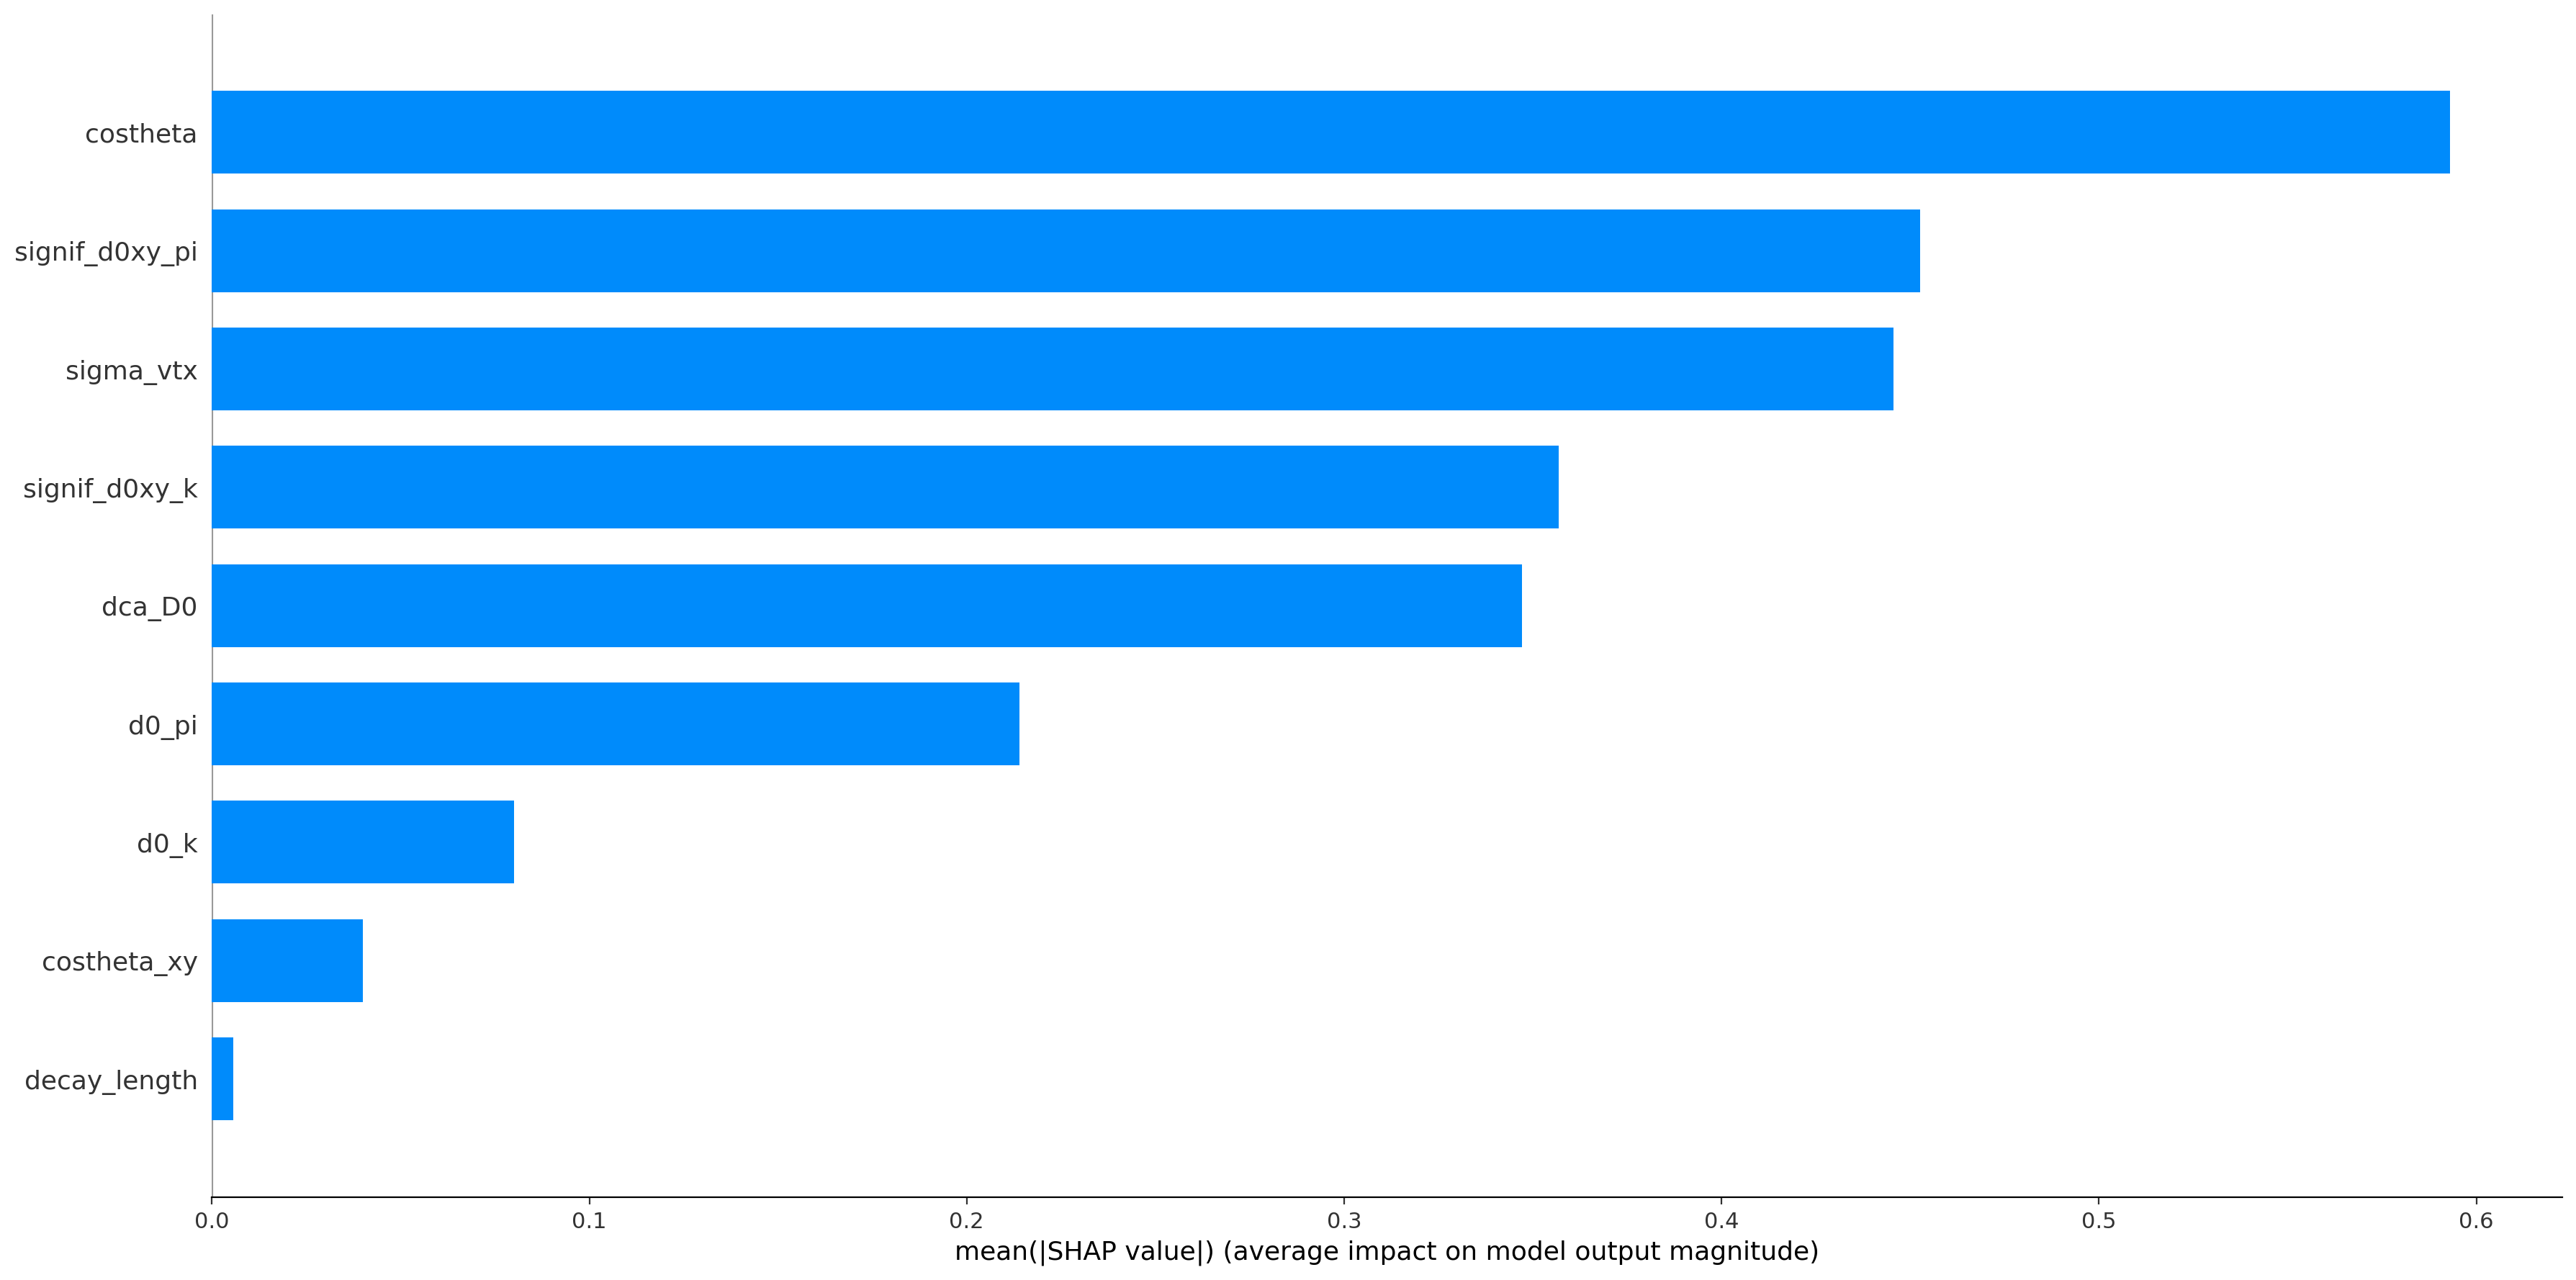
\includegraphics[width=0.95\linewidth]{gallery/ML/ex_shap_feature_impact.png}
    \caption{Example of average SHAP values for topological features used to train a BDT.}
    \label{f.ml_shap}
\end{figure}
%
Fig. \ref{f.ml_shap} summarizes the beeswarm plot by averaging the absolute values of the SHAP results for each candidate. These mean SHAP values provide an overall measure of how much impact each feature has on the BDT outputs, without distinguishing between the particular feature values that push toward signal or background.

%
\begin{figure}[h!]
    \centering
    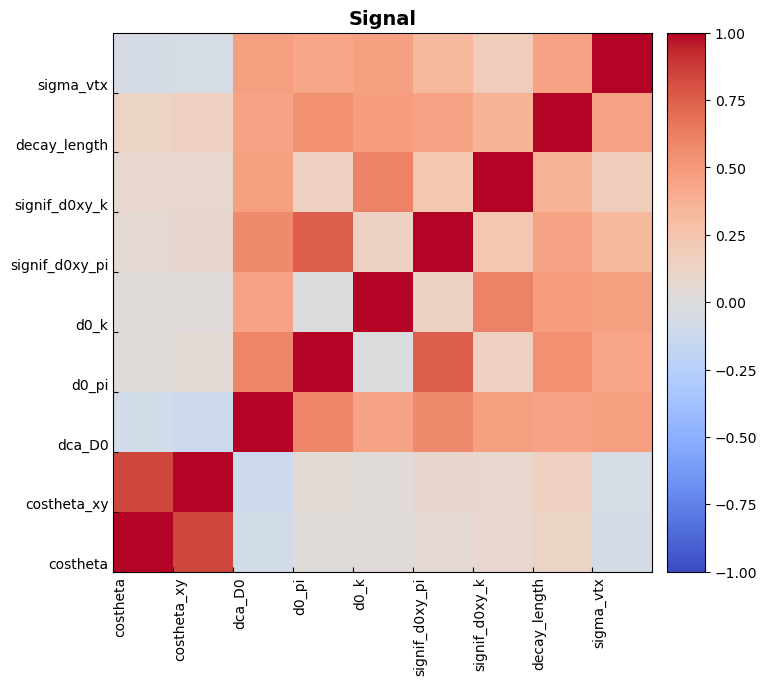
\includegraphics[width=0.7\linewidth]{gallery/ML/ex_correlation_plot_sig.png}
    \caption{Example of feature correlation coefficients. A value of 1 (dark red) indicates perfect positive correlation, and a value of -1 (dark blue) indicates perfect negative correlation.}
    \label{f.ml_corr}
\end{figure}
%
When interpreting SHAP values, it is also important to be cognizant of the correlations between feature values. In Fig. \ref{f.ml_corr}, we plot these feature correlations for the signal candidates. The diagonal entries indicate the correlations of a feature with itself, which are all completely positive as expected. However, we also observe noticeable correlations between different features. In particular, there is very strong positive correlation between \texttt{costheta} and \texttt{costheta\_xy}. This is unsurprising, since $\cos{\theta_{xy}}$ is the component of $\cos{\theta}$ in the $xy$-plane.

Let us now compare the importance of these two correlated features. If $\cos{\theta}$ exhibits very distinct distributions for signal and background candidates and is thus a highly discriminative feature, then we may reasonably expect the same to be true for $\cos{\theta_{xy}}$. However, we notice in Fig. \ref{f.ml_shap} that \texttt{costheta\_xy} has a drastically lower mean SHAP value than \texttt{costheta}. This results from $\cos{\theta_{xy}}$ being very similar to but slightly less discriminative than $\cos{\theta}$, the BDT will tend to cut on $\cos{\theta}$ whenever possible. This leads to $\cos{\theta}$ being rarely used, which artificially suppresses its SHAP value. If we were to train the BDT without including \texttt{costheta}, we would see that \texttt{costheta\_xy} becomes one of the most important features. Thus when features are strongly correlated, their SHAP results should not be taken at face value.

To conclude this section, we note that SHAP is one of many methods that can represent feature importance, and it tends to assign greater importance to features used in the first tree of a BDT, as marginal contributions become increasingly small for trees later on down the boosting chain. Thus, the actual numbers may not be too meaningful, but the plots of SHAP values can nonetheless provide useful qualitative descriptions of how different features impact the model outputs.

%-------------------------
\subsection{Optimizing hyperparameters with Optuna}
\label{sec.ml_optuna}

The final aspect we consider in our analysis is the optimization of hyperparameters, which determine the overall model structure. To determine the most optimal hyperparameter values, we utilize the Optuna package \cite{Optuna}, which tests various points in parameter space and identifies the one which maximizes the ROC AUC of the testing data.

XGBoost provides the following standard BDT hyperparameters \cite{XGBoost_docs}:
\begin{itemize}
    \item \texttt{n\_estimators}: number of trees
    \item \texttt{max\_depth}: maximum depth of each tree
    \item \texttt{learning\_rate} (\texttt{eta}): size of each boosting step
    \item \texttt{min\_child\_weight}: minimum number of candidates in each node
    \item \texttt{min\_split\_loss}: minimum amount of improvement needed to split a node
    \item \texttt{max\_delta\_step}: maximum change in model outputs at each boosting step
    \item \texttt{subsample}: fraction of training data used to train each tree
    \item \texttt{sampling\_method}: algorithm for selecting the subsample for each tree
\end{itemize}
There are also a number of more niche hyperparameters that can be included to adjust the BDT regularization (the conservativeness of the model) and algorithms. For the first three hyperparameters, typical values are on the order of a couple hundred for \texttt{n\_estimators}, 10 or less for \texttt{max\_depth}, and on the order of 0.01 to 0.1 for the \texttt{learning\_rate}. Generally, larger values increase the likelihood of overfitting. By default, values for the other hyperparameters are set such that they provide little to no constraint on the BDT structure. Increasing these values limits the growth or contributions of trees, which is meant to help regularize the model and prevent overfitting.

Although Optuna automates the process of finding the optimal set of hyperparameter values, its results depend on the inputs we provide, such as the combination of hyperparameters we select and the ranges within which we restrict those values.
\chapter{BDT based $D^0$ analyses for the EIC}
\label{ch.results}

This chapter presents the methods and results of the machine learning analyses we performed to separate $D^0$ signals from background. In Ch. \ref{sec.results_gen_methods}, we outline the general analysis methodology and workflow common to all our analyses. In Ch. \ref{sec.results_bkg_study}, we present a preliminary analysis on the impacts of machine-background on $D^0$ invariant mass reconstruction, which we perform by applying an existing BDT framework to new data samples. Then in Ch. \ref{sec.results_optimization}, we present the steps taken to further optimize the framework for our analysis, in terms of the various aspects of BDT implementation discussed in Ch. \ref{sec.ml_implementation}, and discuss our findings.

%---------------------------------------------------------
\section{General methodology}
\label{sec.results_gen_methods}

All data is obtained from PYTHIA-8 simulated $ep$-collisions with $Q^2>1~{\rm GeV^2}$, which are provided by the ePIC Collaboration (ref. in Appendix \ref{app.samples}). We adapt the codes for obtaining $D^0$ signal and background candidates from \cite{Shyam_analysis}, and the machine learning framework from \cite{Shyam_ml}, provided by Shyam Kumar.

We obtain true signal candidates from $D^0$-enriched data samples, in which every collision event produces at least one $D^0$-meson. This rate of $D^0$ production is far above that expected in real $ep$ collisions, but we use this data in order to obtain sufficient signal candidates for training the BDT. We obtain the true background from minimum-bias DIS data samples, meaning that there is no $D^0$-enrichment. We will refer to the $D^0$-enriched data as ``D0 samples" and the minimum-bias data as ``DIS samples."

We combine signal and background candidates into one dataset $\mathcal{D}$, in which each candidate is represented by a vector containing the values of their topological features. We include the same number of signal and background candidates in $\mathcal{D}$ to avoid introducing bias. From $\mathcal{D}$, we randomly select 80\% of the data for $\mathcal{D}_{\rm train}$ and 20\% of the data for $\mathcal{D}_{\rm test}$.

Since we do not have real data to analyze, we estimate the BDT performance by ``applying" the model back on the original data $\mathcal{D}$. For a chosen BDT threshold, we calculate the resulting signal and background {\it efficiencies}, $\epsilon_{\rm{sig}}(\hat{y}^*)$ and $\epsilon_{\rm{bkg}}(\hat{y}^*)$, which are the percentages of signal and background candidates in the test dataset which are accepted by the model for a given BDT threshold $\hat{y}^*$. More concretely, if we start with a dataset $\mathcal{D}$ with $N^{\rm tot}_{\rm sig}$ signal candidates and $N^{\rm tot}_{\rm bkg}$ background candidates, then when we apply the BDT, we select the subset $\mathcal{D}^{\rm ML}$ that contains 
\begin{equation}
\begin{aligned}
    N^{\rm ML}_{\rm sig} &=\epsilon_{\rm sig}(\hat{y}^*) N^{\rm tot}_{\rm sig} \ , \\
    N^{\rm ML}_{\rm bkg} &=\epsilon_{\rm bkg}(\hat{y}^*) N^{\rm tot}_{\rm bkg} \label{eqn.eff}
\end{aligned}
\end{equation}
signal and background candidates.

In order to examine the effectiveness of the signal-and-background separation, we plot the invariant mass distribution of the combined signal and background candidates and look for the $D^0$ peak, which is located around 1.84 ${\rm GeV/c^2}$. For more realistic results, we first use a random sampling method 
(described in Appendix \ref{app.data_prep}) 
to scale up the number of candidates such that they correspond to the expected number of events in EIC experiments, with the desired luminosity of $10~{\rm fb}^{-1}$. We then calculate the S/B (Eq. \eqref{eqn.s_over_b}) and Significance (Eqn. \eqref{eqn.signif}) of the candidates in the $D^0$ peak region, defined to be within two standard deviations on either side of the peak value. We first determine the invariant mass distribution, S/B, and Significance for the initial data before using BDT (using $N_{\rm sig}^{\rm tot}$ and $N_{\rm bkg}^{\rm tot}$), then examine the improvements to these results after applying the BDT (using $N_{\rm bkg}^{\rm ML}$ and $N_{\rm bkg}^{\rm ML}$ ).

%---------------------------------------------------------
\section{Machine-background effects on $D^0$ invariant mass reconstruction: a preliminary analysis}
\label{sec.results_bkg_study}

As a preliminary study, we apply the BDT framework developed in previous work \cite{Shyam_ml} to two new sets of simulated data samples, one set with machine-background effects and one set without those effects. The goal of this study is to examine the impacts of machine background on the $D^0$ analysis. These machine-background effects include interactions between beam particles and gas in beam pipe, electron scattering within the beam, and synchrotron radiation \cite{eic_ptdr}, which produce additional noise in detector measurements. We aim to explore how these effects impact the effectiveness with which BDTs can separate the $D^0$ signals from background by comparing results for data with machine-background effects to those for data without those effects.

%-------------------------
\subsection{Preliminary BDT framework}
\label{sec.results_prelim_methods}

In this preliminary study, we analyze one set of D0 and DIS samples from simulations incorporating machine-background effects, along with a second set of D0 and DIS samples from data without those effects (ref. in Appendix \ref{app.samples}).

We separately train two BDT models---one model for the samples without machine-background effects, and another for the samples with those effects. Here, we analyze all the data in one inclusive kinematic range of $-2<y<3$ and $p_T>1$. We utilize the following 10 topological features, which characterize the $D^0\rightarrow\pi+K$ decay, depicted in Fig. \ref{f.d0_decay_diagram_2}:
\begin{multicols}{2}
\begin{itemize}
    \item \texttt{costheta}: $\cos{\theta}$
    \item \texttt{costheta\_xy}: $\cos{\theta_{xy}}$
    \item \texttt{decay\_length}: Decay Length
    \item \texttt{dca\_D0}: $\rm DCA_{D0}$
    \item \texttt{d0\_pi}: $\rm DCA_\pi$
    \item \texttt{d0\_k}: $\rm DCA_K$
    \item \texttt{d0xy\_pi}: ${\rm DCA_\pi}_{(xy)}$
    \item \texttt{signif\_d0xy\_pi}: ${\rm DCA_\pi}_{(xy)}/\sigma_\pi$
    \item \texttt{signif\_d0xy\_k}: ${\rm DCA_K}_{(xy)}/\sigma_K$
    \item \texttt{sigma\_vtx}: $\sigma$ of decay vertex
\end{itemize}
\end{multicols}
where $\sigma$ represents the associated uncertainty for a given variable. Often, the variables normalized by $\sigma$ may be provide more accurate representations of signal vs. background candidates. The \texttt{sigma\_vtx} feature is the uncertainty associated with the decay vertex location, where the vertex is taken to be the midpoint of the line defining ${\rm DCA_{12}}$. 

%
\begin{figure}[h!]
    \centering
    \includegraphics[width=0.6\linewidth]{gallery/D0_topology/d0_decay.png}
    \caption{$D^0\rightarrow \pi^+ + K^-$ decay in the transverse plane. The labelled topological features are defined in Ch. \ref{sec:def_top_vars}. Figure from the STAR Collaboration \cite{STAR}.}
    \label{f.d0_decay_diagram_2}
\end{figure}
%

We do not include all the available topological features, but adopt the preferred combination of features as determined in previous work. When applying the BDT model, we choose a threshold BDT output of 0.6, which is also the best value determined in previous work.

Here, we note that the particular kinematic range, topological feature selection, and BDT threshold are choices that have been optimized for previous work analyzing different data, so these choices are likely not the most effective for our analysis. In the subsequent analyses of Ch. \ref{sec.results_optimization}, we aim to optimize these choices for our particular data samples.


% \begin{equation}
%     eff_{\rm sig(bkg)} = \frac{N_{\rm sig(bkg)}\left[\hat{y}>\hat{y}^* \right]}{N_{\rm sig(bkg)}\left[\hat{y}\geq 0 \right]} \ ,
% \end{equation}
% where the numerator is the number of candidates accepted by the BDT for a given threshold $\hat{y}^*$, and the denominator is the total number of candidates/ 

%-------------------------
\subsection{BDT training}

To assess the performances of the BDT models, we examine the BDT outputs and ROC curves for the training vs. testing datasets, which we introduced in Ch. \ref{sec.ml_performance}.

%
\begin{figure}[h!]
    \centering
    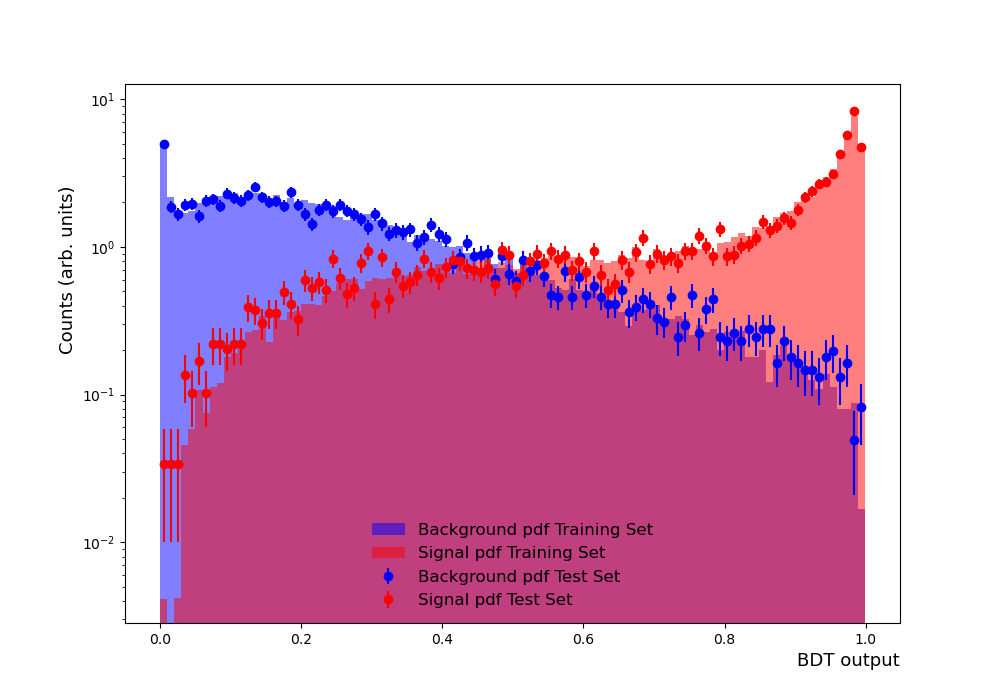
\includegraphics[width=0.5\linewidth]{gallery/results/train_test_without_bkg.png}
    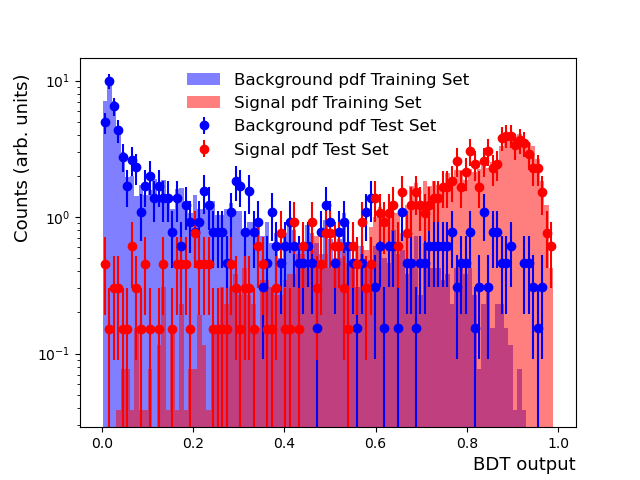
\includegraphics[width=0.46\linewidth]{gallery/results/train_test_with_bkg.png}
    \caption{BDT output distributions of training vs. test data for samples without (left) and \textbf{with (right)} machine-background effects. In both plots, training data are plotted as shaded histograms and test data are plotted as solid markers, with background candidates in blue and $D^0$ signal candidates in red.}
    \label{f.bkg_study_bdt_score}
\end{figure}
%
Fig. \ref{f.bkg_study_bdt_score} compares the BDT output distributions for the samples with and without machine-background effects. In the results for samples without machine-background effects (left plot), we observe that the distributions for training and testing data follow each other closely, which indicates that the BDT model results are consistent across both datasets. However, for the samples {\textbf{with}} machine-background effects (the right-side plots), we notice much greater discrepancy between the outputs for training and testing data near the tail ends of each distribution, which indicates that the model is less stable. We also see that the distributions for the samples {\textbf{with}} machine-background effects are less strongly peaked near 0 and 1, which suggests that the discriminatory ability of this BDT model is weaker. This is likely because the topological distributions of signal and background look more similar as a result of the machine-background effects.

%
\begin{figure}[h!]
    \centering
    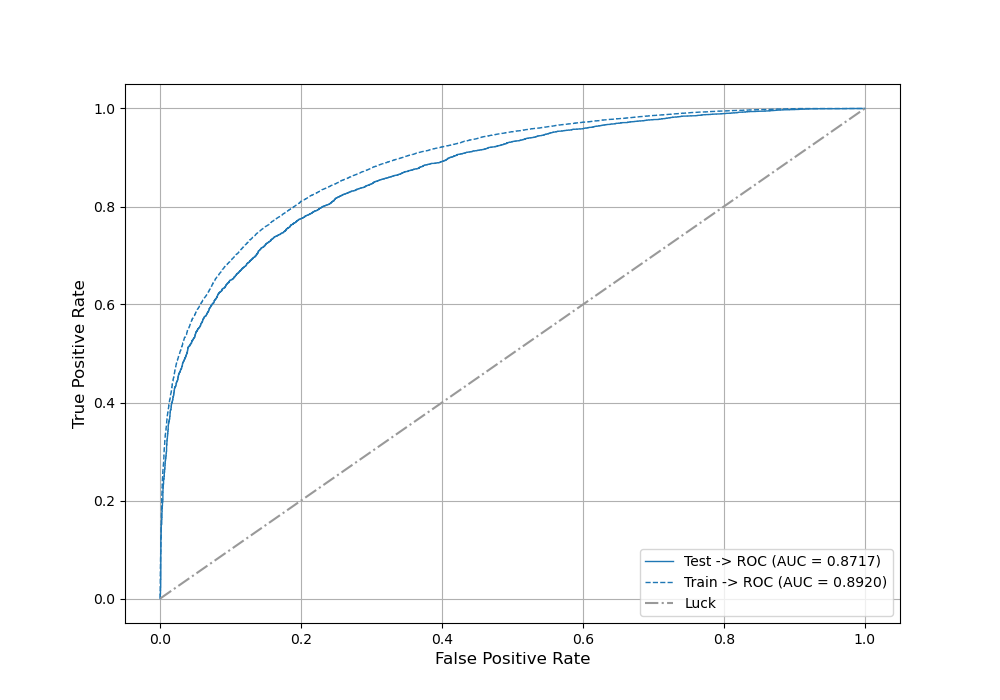
\includegraphics[width=0.5\linewidth]{gallery/results/roc_train_test_without_bkg.png}
    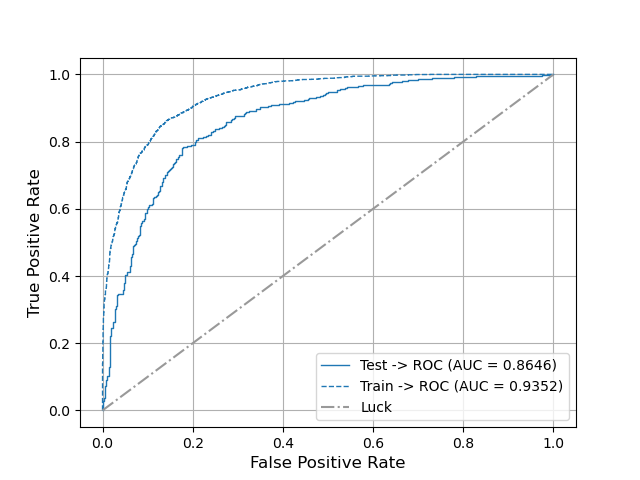
\includegraphics[width=0.46\linewidth]{gallery/results/roc_train_test_with_bkg.png}
    \caption{ROC curves for training (dashed line) vs. test data (solid line). The left plot shows results for samples without machine-background effects (Test ${\rm AUC}=0.8717$, Train ${\rm AUC}=0.8920$), and the right plot shows results for samples \textbf{with} machine-background effects (Test ${\rm AUC}=0.8646$, Train ${\rm AUC}=0.9352$).}
    \label{f.bkg_study_roc}
\end{figure}
%
Fig. \ref{f.bkg_study_roc} compares the ROC curves of the BDT models for the two data samples. In both cases, the ROC AUC for the training data and the testing data are well above 0.8, so both BDT models achieve good performance. However, for the samples \textbf{with} machine-background effects, there is significant discrepancy between the ROC curves of the training and testing data, which indicates overfitting.

%-------------------------
\subsection{Results for data with vs. without machine-background effects}

%
\begin{figure}[h!]
    \centering
    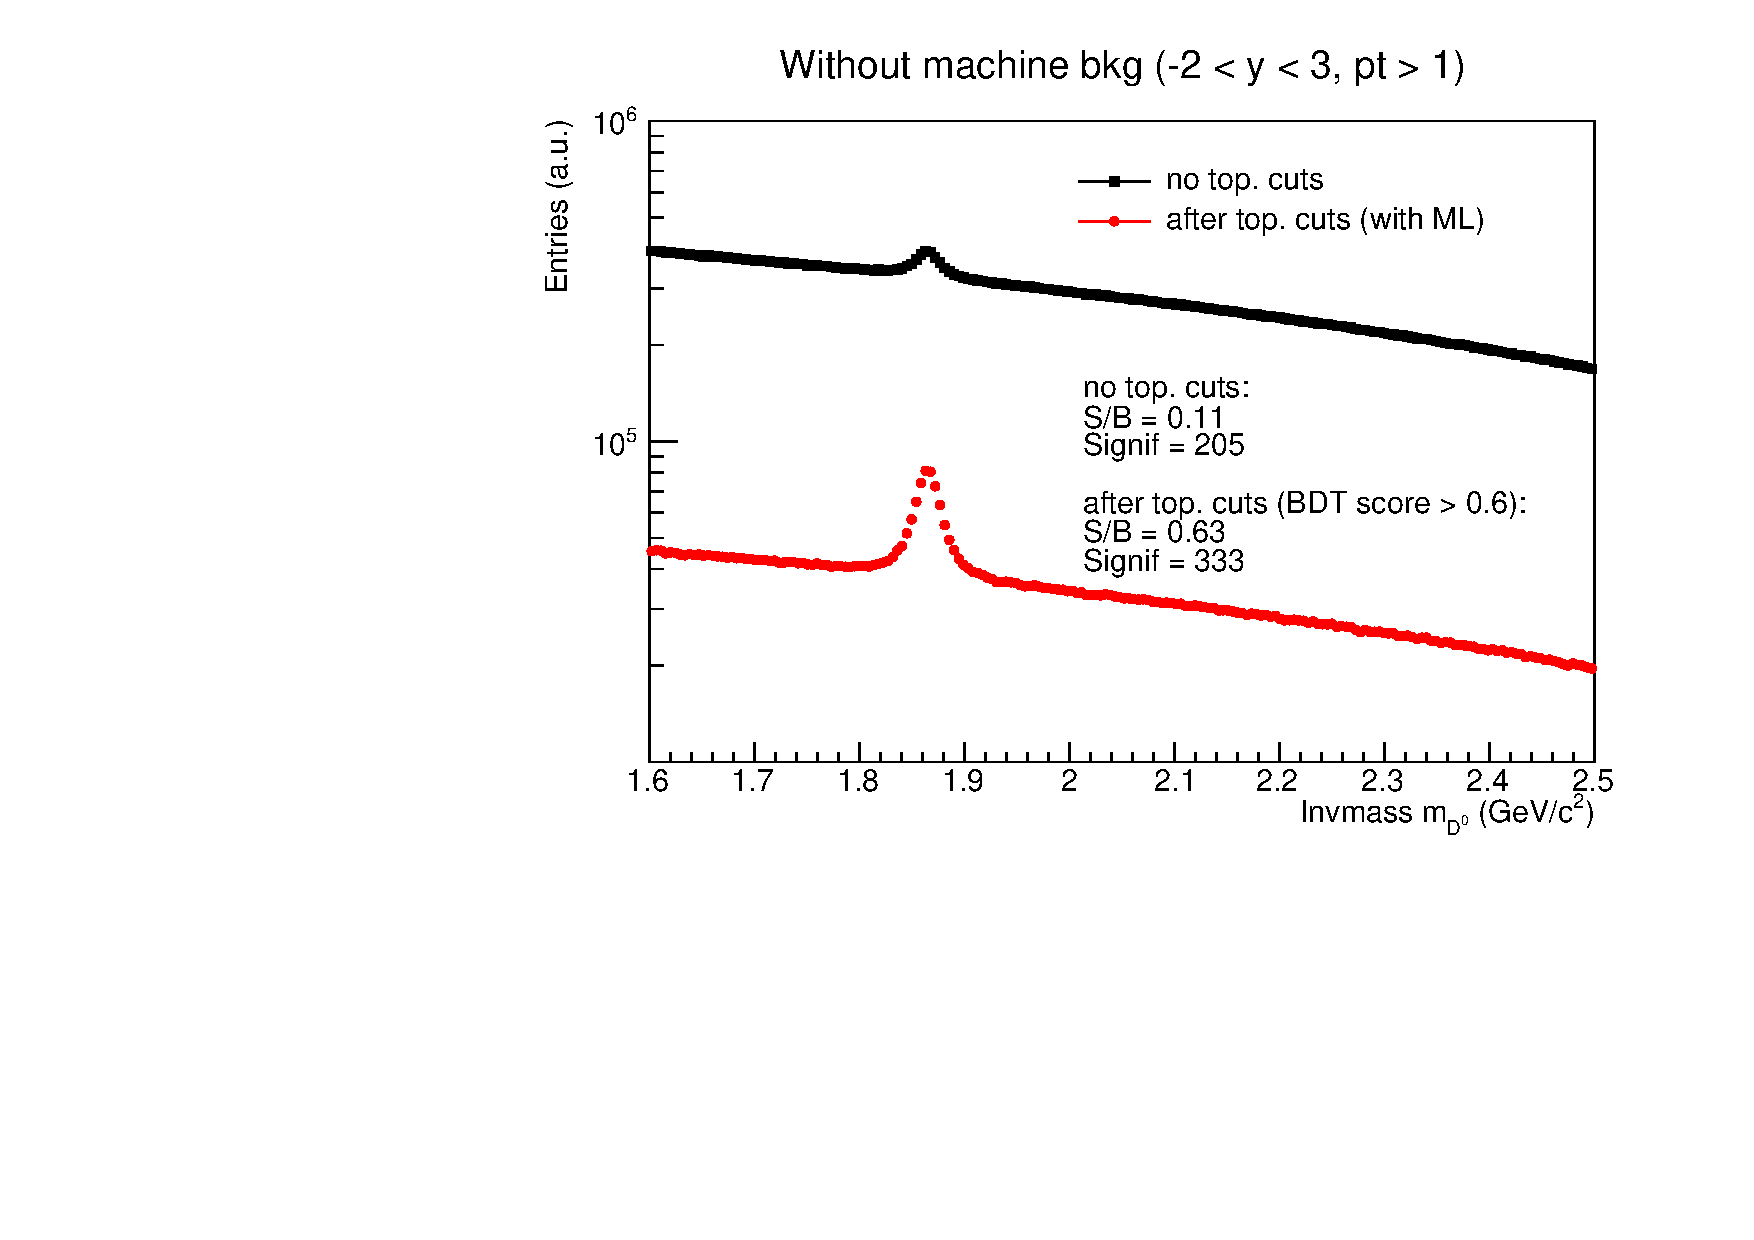
\includegraphics[width=0.6\linewidth]{gallery/results/inv_mass_without_bkg.pdf}
    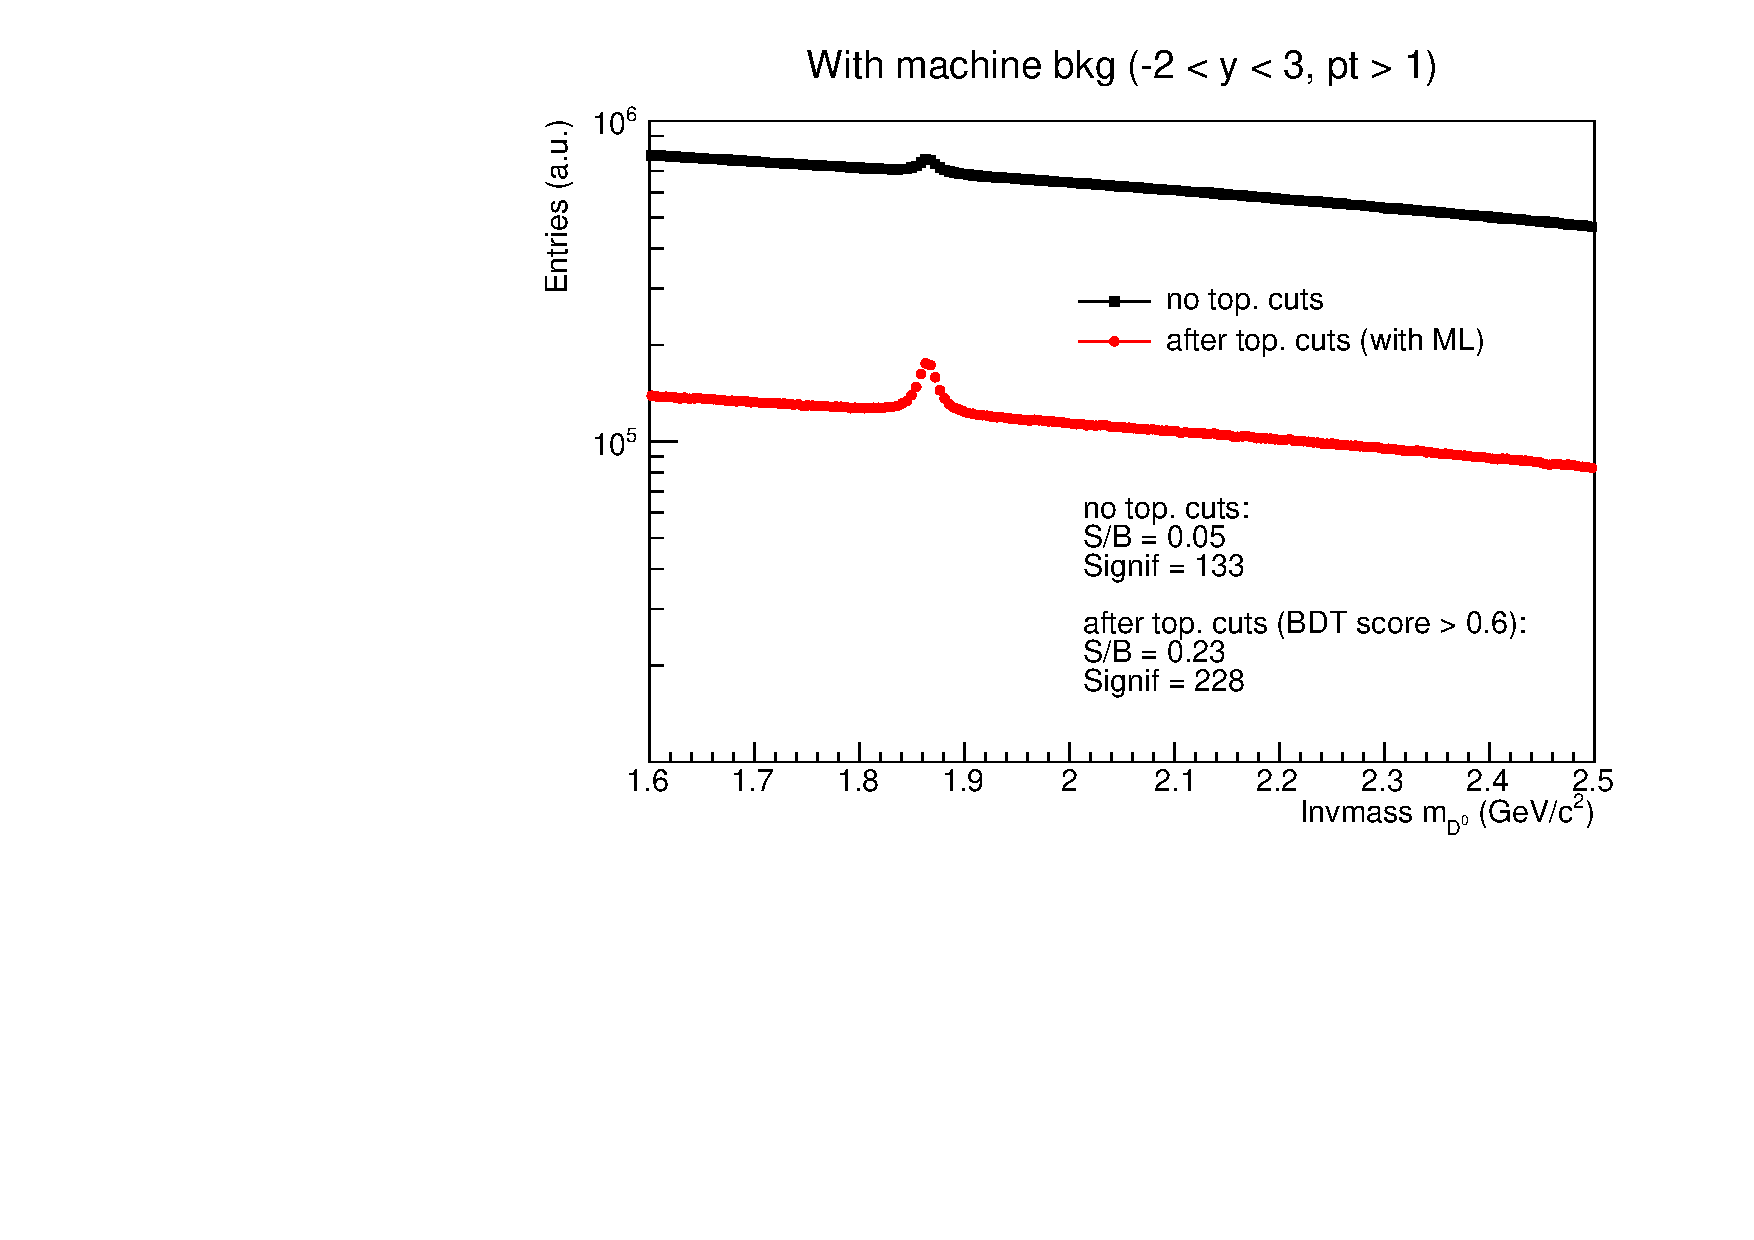
\includegraphics[width=0.6\linewidth]{gallery/results/inv_mass_with_bkg.pdf}
    \caption{Reconstructed $D^0$ invariant mass distributions before (black) vs. after (red) BDT, for samples without (top plot) and \textbf{with (bottom plot)} machine-background effects. In both samples, the plots after BDT correspond to candidates with BDT output $> 0.6$.}
    \label{f.bkg_study_inv_mass}
\end{figure}
%
Fig. \ref{f.bkg_study_inv_mass} compares the resampled invariant mass distributions before using BDT (black) and after applying BDT selections (red). We see that for both the samples \textbf{with} and without machine-background effects, applying BDT improves the S/B and Significance, with approximately a 60\% increase in Significance for the samples without machine-background effects, and a 70\% increase in Significance for the samples \textbf{with} machine-background effects. Thus, we can see more prominent $D^0$ peaks after applying BDT. Comparing the two data samples, we observe that the data \textbf{with} machine-background effects have much higher background baselines, and S/B and Significance are unfortunately much lower. This illustrates the negative impact of the machine-background effects on the efficiency with which we can reconstruct the $D^0$ invariant mass peak.

%
\begin{figure}[h!]
    \centering
    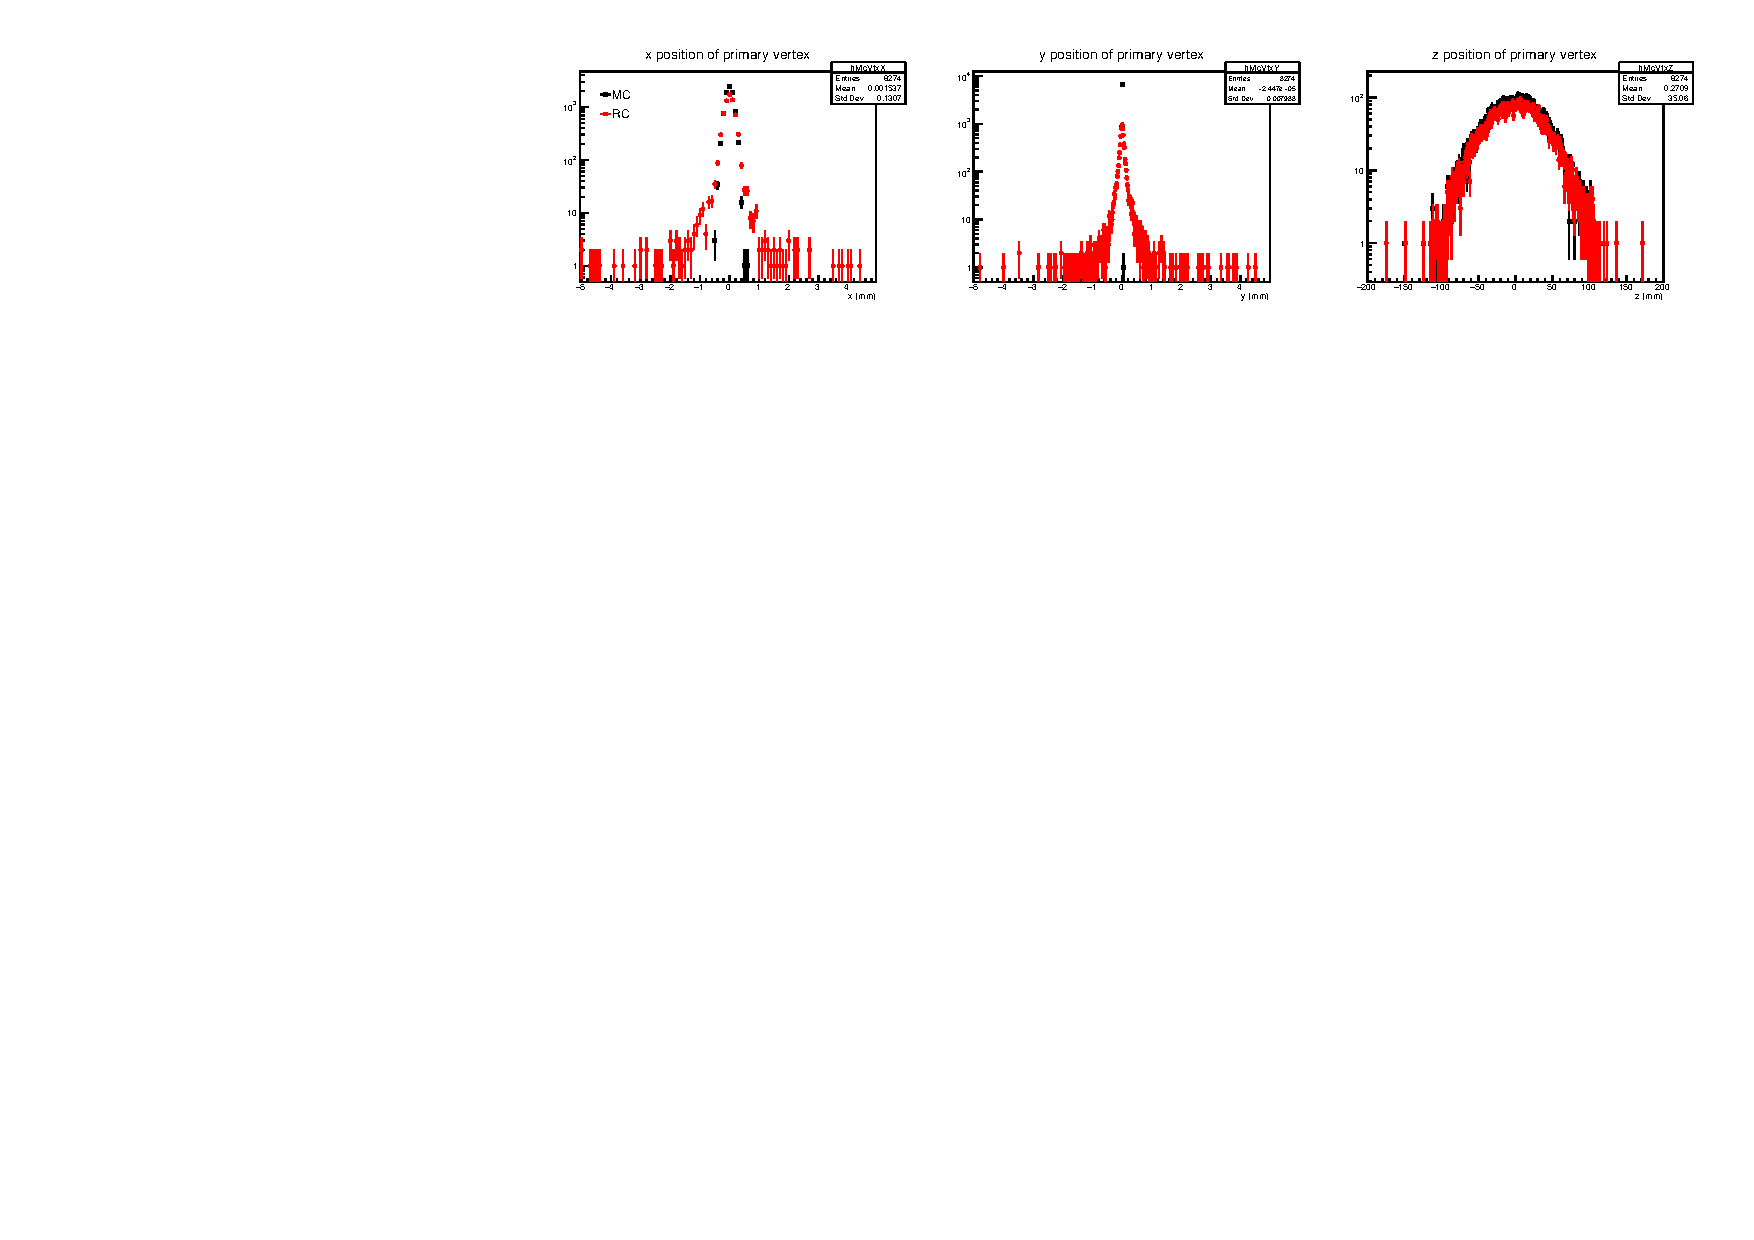
\includegraphics[width=0.95\linewidth]{gallery/results/prim_vtx_DIS_without_bkg.pdf}
    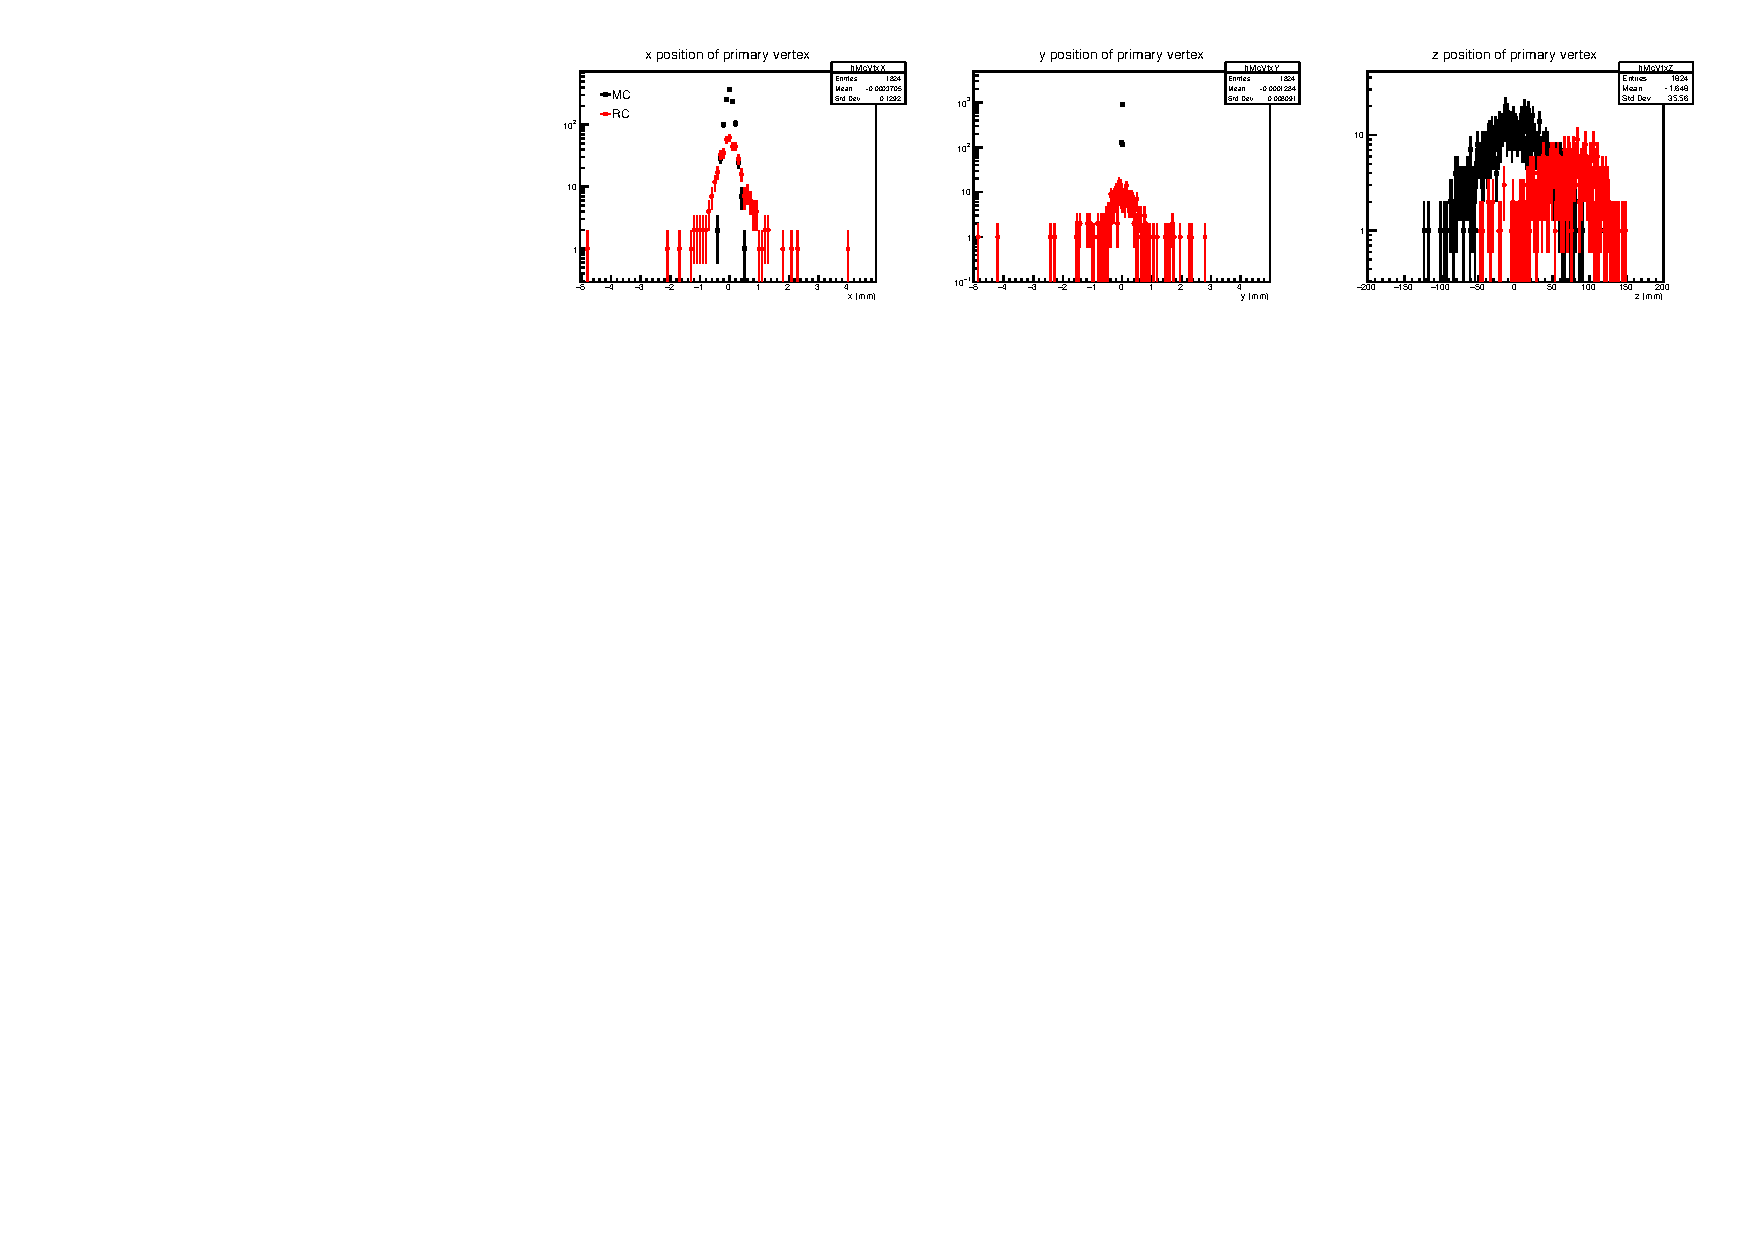
\includegraphics[width=0.95\linewidth]{gallery/results/prim_vtx_DIS_with_bkg.pdf}
    \caption{Comparisons of $x$, $y$, and $z$ locations of the reconstructed (RC) primary vertices vs. the true Monte Carlo (MC) vertices. The top shows data without machine-background effects, and the bottom shows data \textbf{with} machine-background effects.}
    \label{f.prim_vtx}
\end{figure}
%
During this study, we also found a shortcoming in the reconstruction of data \textbf{with} machine-background effects. In Fig. \ref{f.prim_vtx}, we compare the reconstructed primary vertex locations (red) to the true locations given by the Monte Carlo simulations (black). The $x$- and $y$- distributions of the reconstructed vertices are consistent with the distributions we expect from the Monte Carlo results, just with larger spreads due to reconstruction uncertainty. However, we observe that the $z$-distribution of the primary vertex for samples \textbf{with} machine-background effects (bottom right plot) is shifted off-center from the expected location. This inaccuracy of the primary vertex location leads to less reliable values for the $D^0 \rightarrow\pi+K$ topological features, which contributes to the much lower efficiency of $D^0$ signal-and-background separation. Thus, adjustments to the primary vertex reconstruction methodology is needed to improve the $D^0$ analysis.

%---------------------------------------------------------
\section{Optimizing the analysis for various slices of $y$ and $p_T$ of the $D^0$}
\label{sec.results_optimization}

To further increase the efficiency of $D^0$ signal-and-background separation, we aim to improve upon the preliminary BDT methodology (described in Ch. \ref{sec.results_prelim_methods}) in three ways:
\begin{enumerate}
    \item Analyzing the data in slices of $y$ and $p_T$, and optimizing the BDT threshold for each slice
    \item Determining the most effective combination of topological features
    \item Tuning BDT hyperparameters to adjust the model structure
\end{enumerate}
We address each of these aspects in this section.

%---------------------------
\subsection{Preliminary results in various $y$ and $p_T$ slices}
\label{sec.results_prelim}

In Ch. \ref{ch:d0_top}, we established that the $D^0\rightarrow\pi+K$ topology depends on the $y$ and $p_T$ of the $D^0$. Thus, we move forward with the analysis by dividing the data into different kinematic slices (Table \ref{tab.kinematics}):

\begin{center}
\begin{tabular}{c|c|c}
            & $-1<y<1$ & $1<y<3$ \\
            \hline
$1<p_T<2~{\rm GeV/c}$   & mid-$y$, low $p_T$ & forward $y$, low $p_T$ \\
$2<p_T<3~{\rm GeV/c}$   & mid-$y$, high $p_T$ & forward $y$, high $p_T$ \\
\end{tabular}
\end{center}

For each slice, we train a separate BDT model and optimize the BDT threshold by selecting the value that yields the highest Significance. (Here, we continue to use the same topological features and BDT hyperparameters as in the preliminary analysis.) Fig. \ref{f.inv_mass_slices} shows the $D^0$ invariant mass distributions obtained for each slice.

%
\begin{figure}[h!]
    \centering
    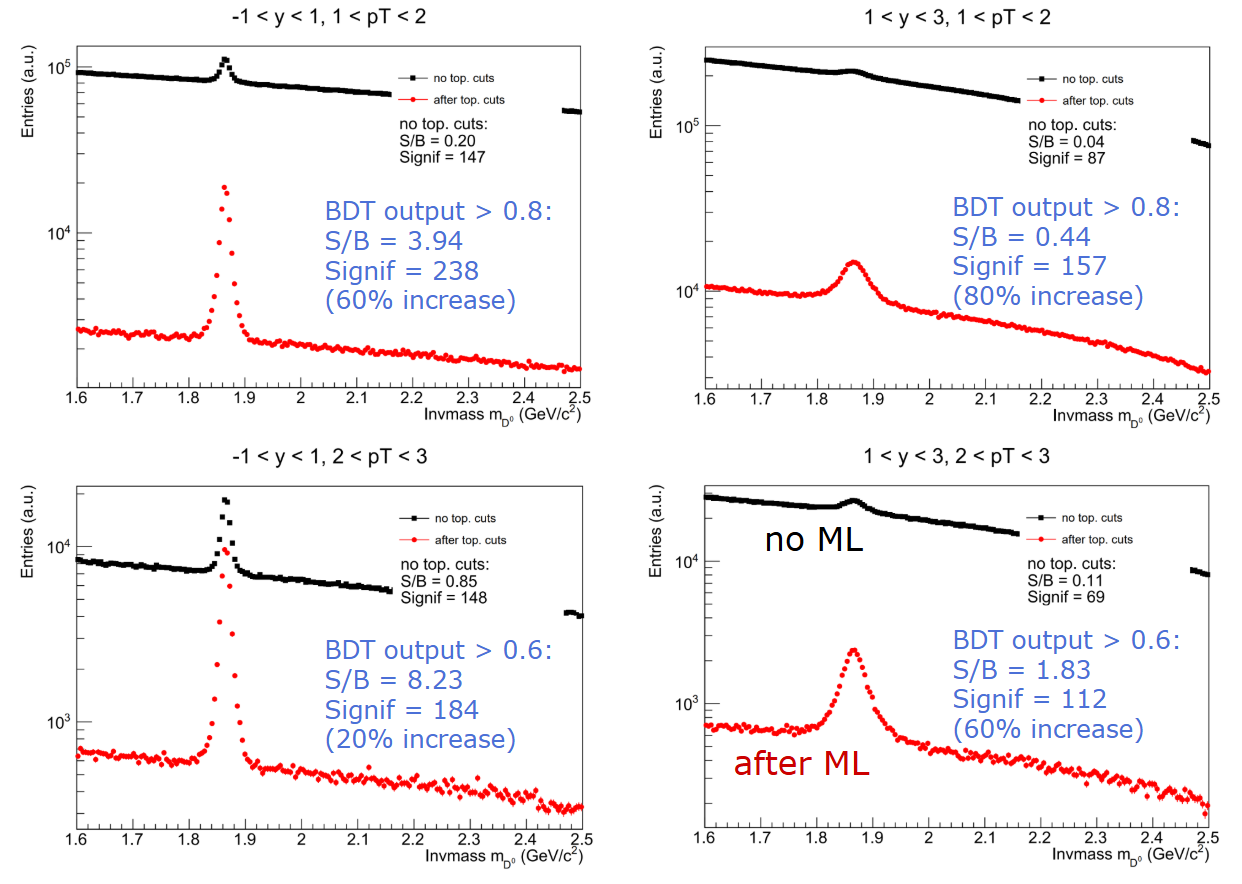
\includegraphics[width=0.9\linewidth]{gallery/results2/inv_mass_slices.png}
    \caption{Reconstructed $D^0$ invariant mass distributions before (black) vs. after (red) BDT, in various slices of $y$ and $p_T$ of the $D^0$. The BDT threshold for each slice is chosen to give the highest Significance. The \% increase denotes the change in Significance from before BDT to after BDT.}
    \label{f.inv_mass_slices}
\end{figure}
%
We observe that the resolution of the $D^0$ peak differs in each of the four slices, and the improvement in results after applying BDT also varies. Comparing low $p_T$ vs. high $p_T$ for the same $y$ range (top row vs. bottom row), we find that the high $p_T$ slice yields a higher S/B and lower Significance. This can be explained by the reconstruction of the $D^0\rightarrow \pi+K$ decay being more accurate for high $p_T$ particles, but the statistics being much lower at high $p_T$. These factors result in cleaner signal-and-background separation but larger statistical uncertainties. Comparing mid-$y$ vs. forward $y$ for the same $p_T$ range (left column vs. right column), we find that the forward $y$ yields markedly lower values of S/B and Significance. This is due to the much lower reconstruction efficiency and higher background levels in this region.

Finally, comparing the results before BDT vs. after BDT, we find that the slice which starts with the best S/B before BDT, the mid-$y$ and high $p_T$ slice (bottom left), experiences the smallest improvement after BDT, with only a 20\% increase in the Significance. Conversely, the slice with the lowest S/B before BDT, the forward $y$ and low $p_T$ slice (top right), experiences the greatest improvement after BDT, with an 80\% increase in Significance. These results indicate the BDT has the most potential for impact for this kinematic region in which the reconstruction is most difficult.

%---------------------------
\subsection{Testing various feature selections}
\label{sec.results_features}

For each kinematic slice, we then tested different combinations of topological features. In total, there are 13 features available (see Fig. \ref{f.d0_decay_diagram_2}):
\begin{multicols}{2}
\begin{itemize}
    \item \texttt{costheta}: $\cos{\theta}$
    \item \texttt{costheta\_xy}: $\cos{\theta_{xy}}$
    \item \texttt{decay\_length}: Decay Length
    \item \texttt{dca\_D0}: ${\rm DCA_{D0}}$
    \item \texttt{d0\_pi}: ${\rm DCA_\pi}$
    \item \texttt{d0xy\_pi}: ${\rm DCA}_{{\rm\pi}(xy)}$
    \item \texttt{signif\_d0xy\_pi}: ${\rm DCA}_{{\rm\pi}(xy)}/\sigma_\pi$
    \item \texttt{d0\_k}: ${\rm DCA_K}$
    \item \texttt{d0xy\_k}: ${\rm DCA}_{{\rm K}(xy)}$
    \item \texttt{signif\_d0xy\_k}: ${\rm DCA}_{{\rm K}(xy)}/\sigma_K$
    \item \texttt{sum\_d0xy}: $\sqrt{{\rm DCA}^2_{{\rm \pi}(xy)}+{\rm DCA}^2_{{\rm K}(xy)}}$
    \item \texttt{dca\_12}: ${\rm DCA_{12}}$
    \item \texttt{sigma\_vtx}: $\sigma$ of decay vertex
\end{itemize}
\end{multicols}

We first trained a BDT using all 13 features. We then examined the average SHAP values (introduced in Ch. \ref{sec.ml_shap}) to determine the most important features, then trained another BDT using only the top 5 features. Finally, we trained an additional BDT using a selection of 9 features:
\begin{multicols}{2}
\begin{itemize}
    \item \texttt{costheta}
    \item \texttt{costheta\_xy}
    \item \texttt{decay\_length}
    \item \texttt{dca\_D0}
    \item \texttt{d0\_pi}
    \item \texttt{signif\_d0xy\_pi}
    \item \texttt{d0\_k}
    \item \texttt{signif\_d0xy\_k}
    \item \texttt{sigma\_vtx}
\end{itemize}
\end{multicols}
These are slightly different from the original 10 features used in the preliminary analysis (listed Ch. \ref{sec.results_prelim}).

%
% \begin{figure}[h!]
%     \centering
%     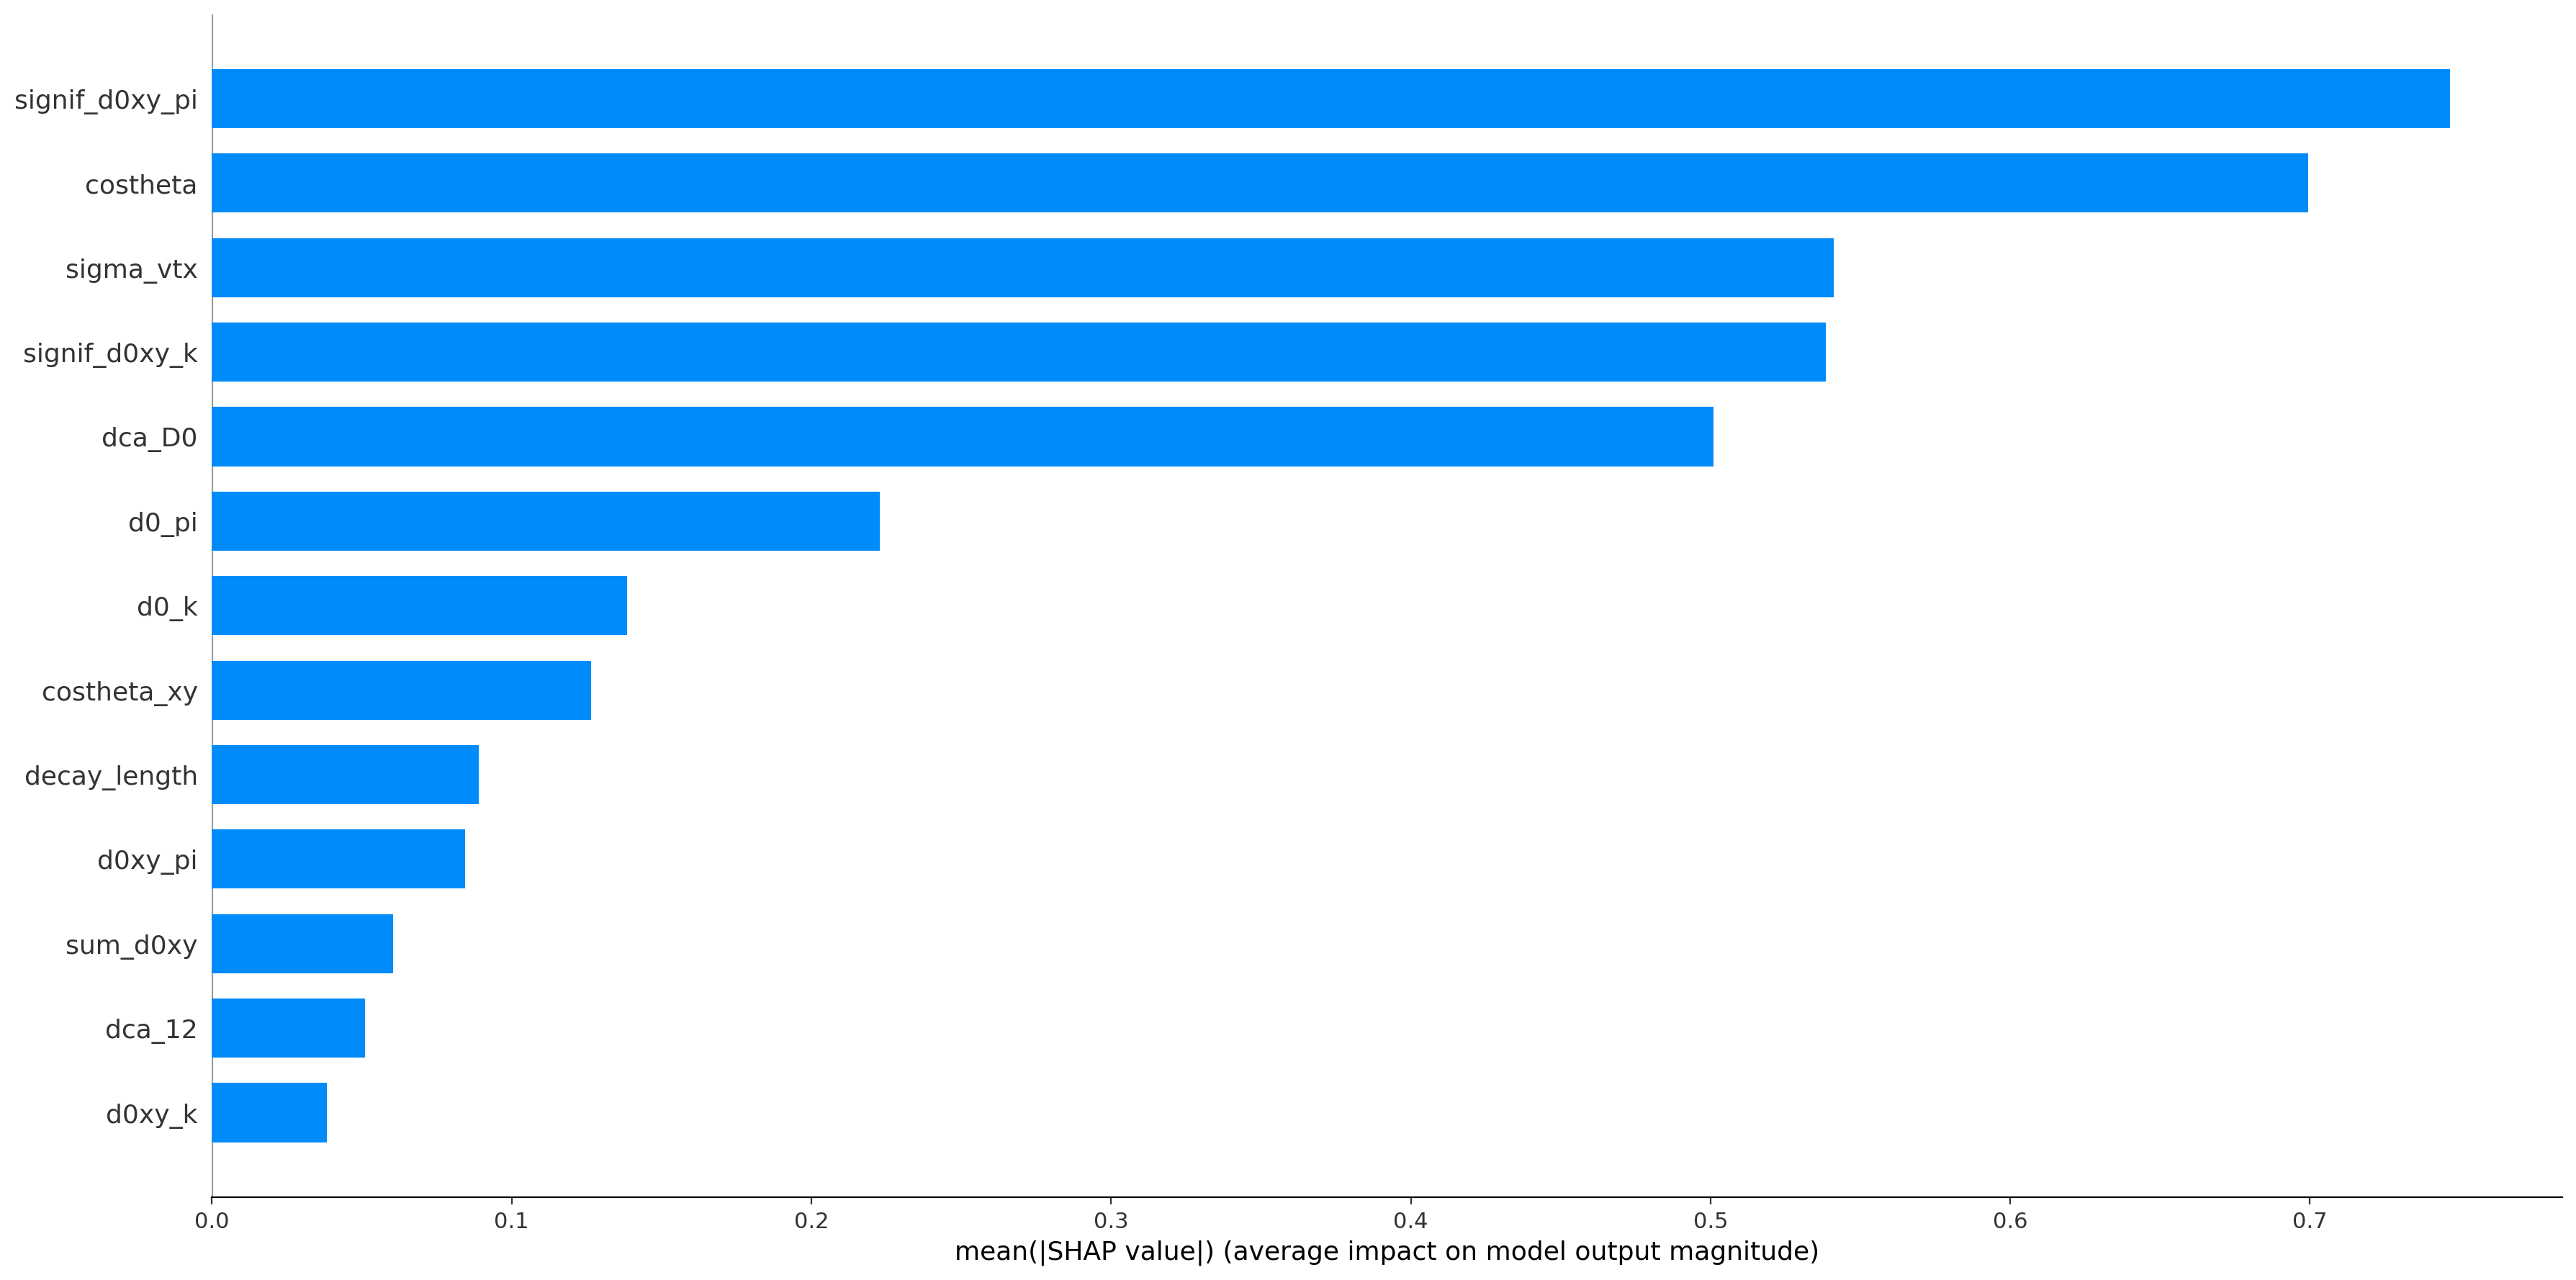
\includegraphics[width=0.95\linewidth]{gallery/results2/all_shap_feature_impact.png}
%     \caption{Average SHAP values of all 13 topological features for $1<y<3$ and $1<p_T<3$.}
%     \label{f.all_shap}
% \end{figure}
%

%
\begin{figure}[h!]
    \centering
    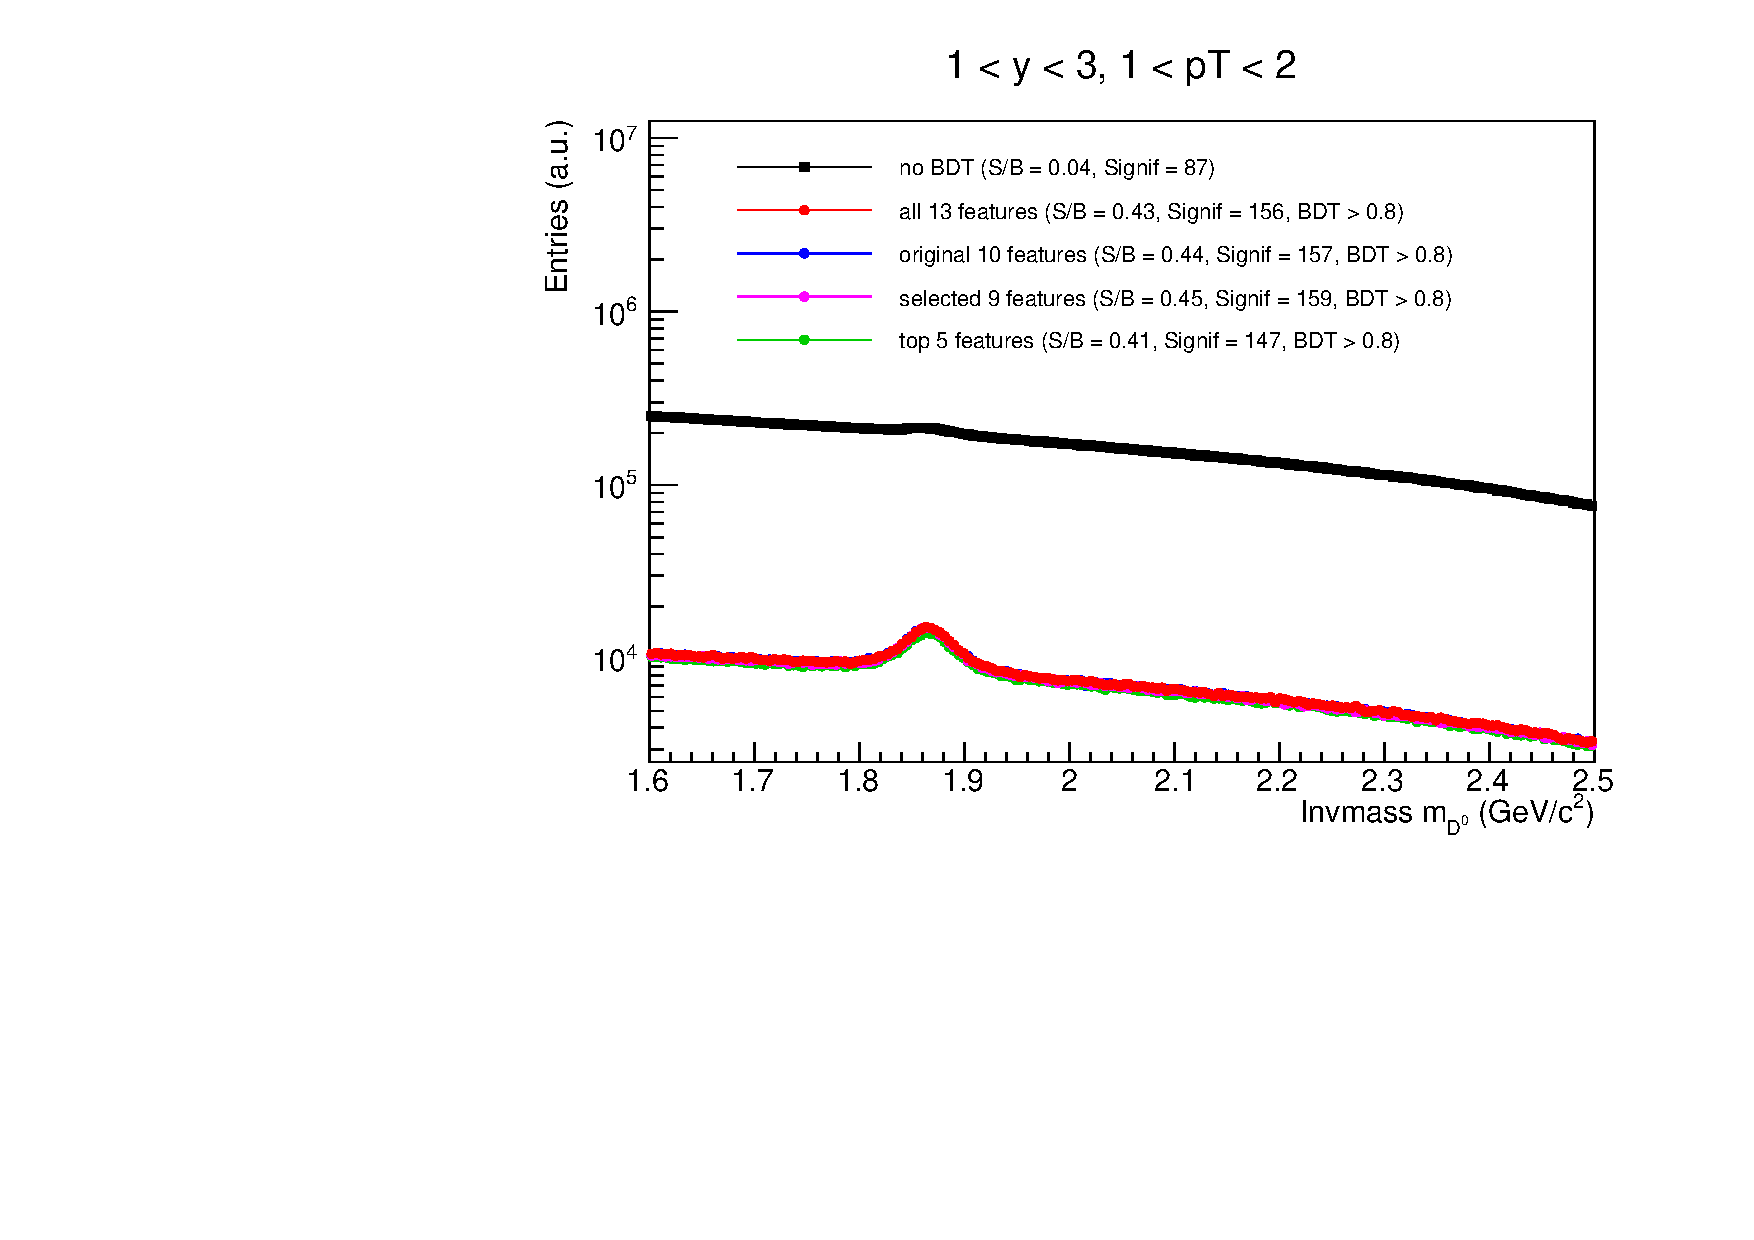
\includegraphics[width=0.65\linewidth]{gallery/results2/inv_mass_diff_features_y_1.0_3.0_pt_1.0_2.0_bdt_0.8.pdf}
    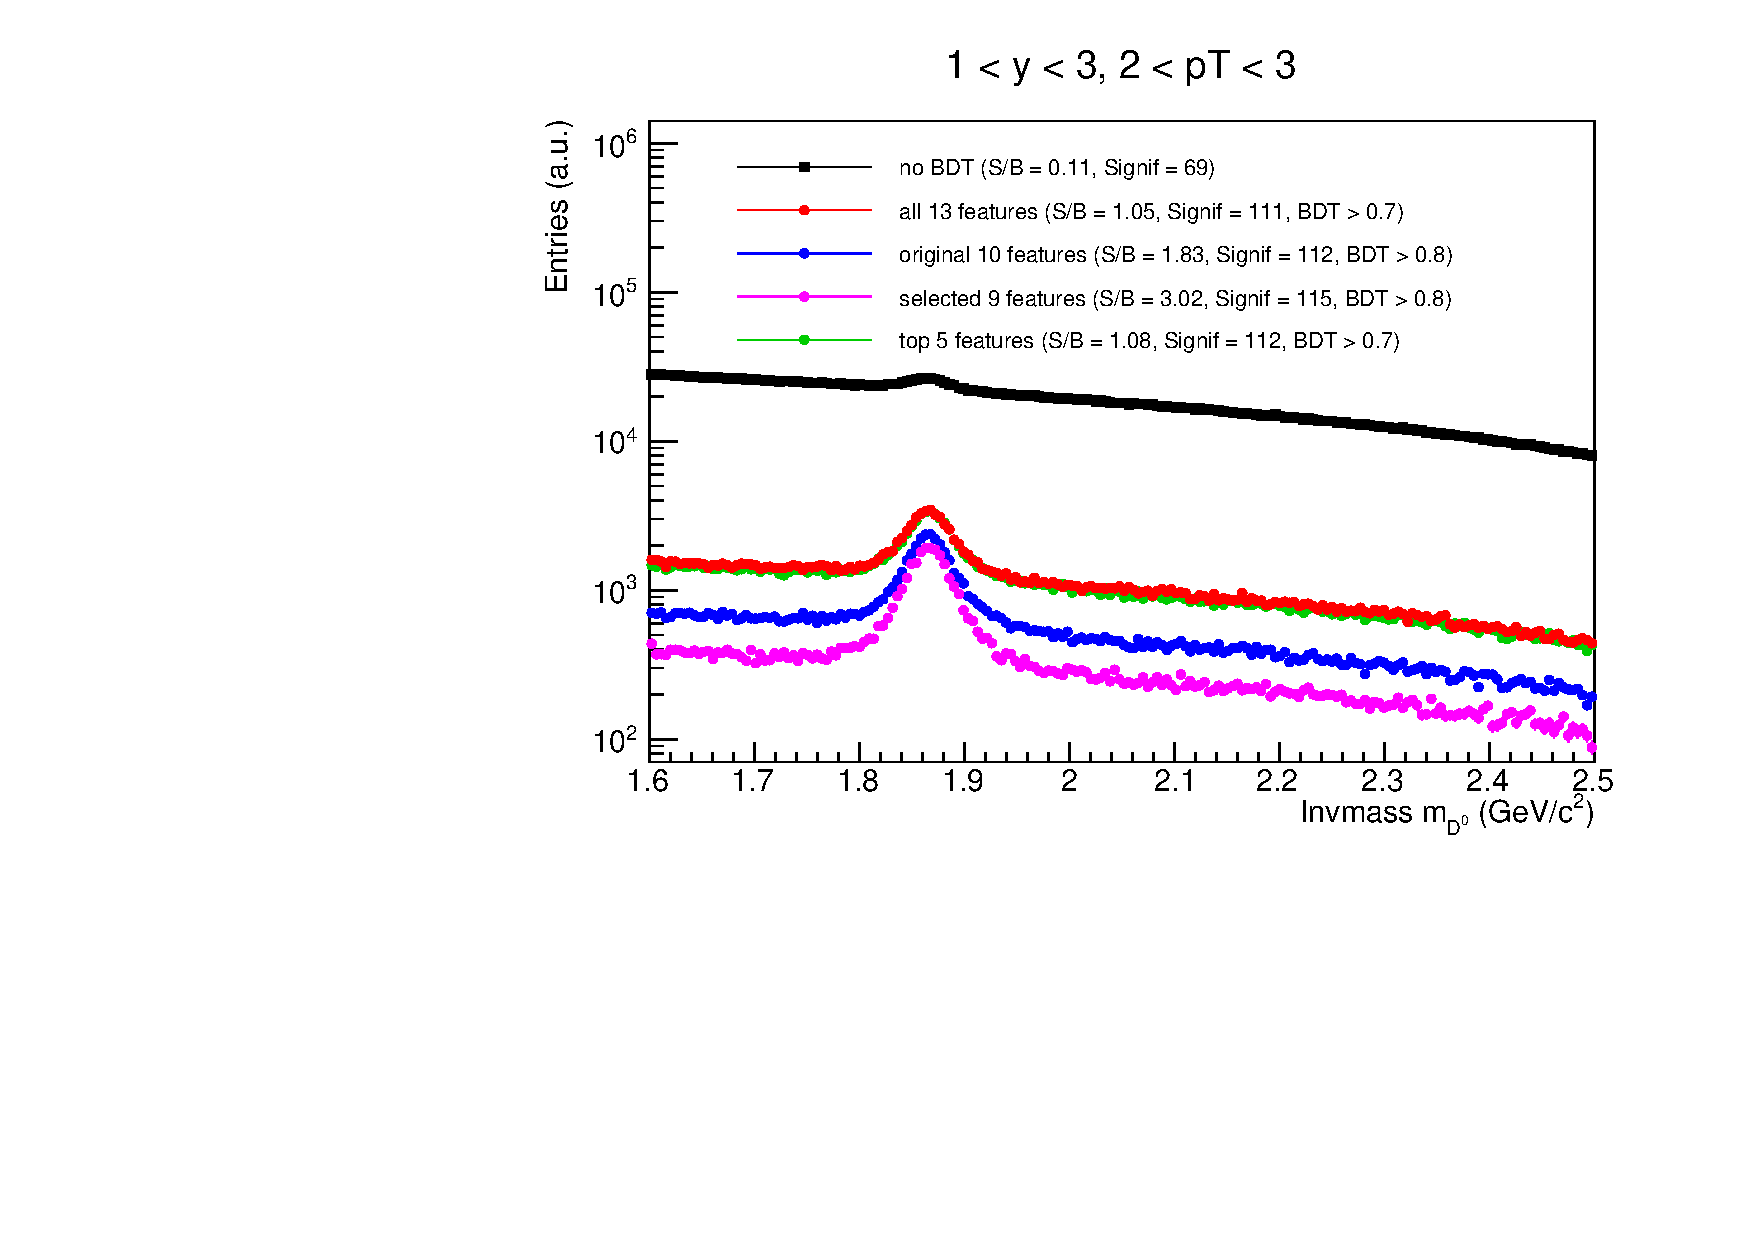
\includegraphics[width=0.65\linewidth]{gallery/results2/inv_mass_diff_features_y_1.0_3.0_pt_2.0_3.0_bdt_0.7.pdf}
    \caption{Reconstructed $D^0$ invariant mass distributions before BDT (black) vs. after applying BDTs trained using various features selections: all 13 available features (red), the original 10 preliminary features (blue), a selection of 9 features (magenta), and the top 5 most important features (green). The top plot shows data for $1<y<3$ and $1<p_T<2~{\rm GeV/c}$, and the bottom plot shows data for $1<y<3$ and $2<p_T<3~{\rm GeV/c}$. Each BDT threshold is selected to yield the highest Significance.}
    \label{f.feature_selections}
\end{figure}
%
Fig. \ref{f.feature_selections} shows examples of the resulting $D^0$ invariant mass distributions obtained using BDTs trained with these various feature combinations. For the forward $y$ and high $p_T$ slice (top plot), we observe that all these different feature selections produce the same results. However, for the high $p_T$ slice (bottom plot), we do notice an impact of feature selection. In particular, the BDT trained using the selection of 9 features (magenta) yields the highest S/B and Significance, thus distinguishing this selection to be the best combination of features for this kinematic slice. The BDT trained using the original 10 features (blue) yields the second best results. Interestingly, the BDT trained using all 13 available features (red) and that trained using only the top 5 features (green) both produce similar results, which are worse than the other two models.

From these results, we can conclude that simply including more features will not necessarily improve BDT performance. This is perhaps unsurprising, as once the most important features are included, any additional features will only produce a small impact on the BDT outputs. Thus, in some instances, the best choice of features is somewhat arbitrary. This is more likely the case for kinematic regions with high statistics, in which the BDT has a sufficiently large training dataset to learn the true signal-and-background boundaries (provided that a few of the most important features are included).

However, the results for the high $p_T$ slice also demonstrate that BDT performance can sometimes worsen as more features are added. This issue tends to arise in such regions with lower statistics, in which the data contains more statistical fluctuations and the BDT is thus more sensitive to feature selection. This might be because providing the BDT with a large number of features gives the model too much flexibility in fitting the training data, which increases the likelihood of overfitting and thus leads to worse performance on testing data. Kinematic regions with high statistics are generally more robust to this issue.

% We can find some explanation for this observation in the BDT output distributions of Fig. \ref{f.bdt_all_vs_fav}, comparing the model trained using the selected 9 features and the model trained using all 13 features.
% %
% \begin{figure}[h!]
%     \centering
%     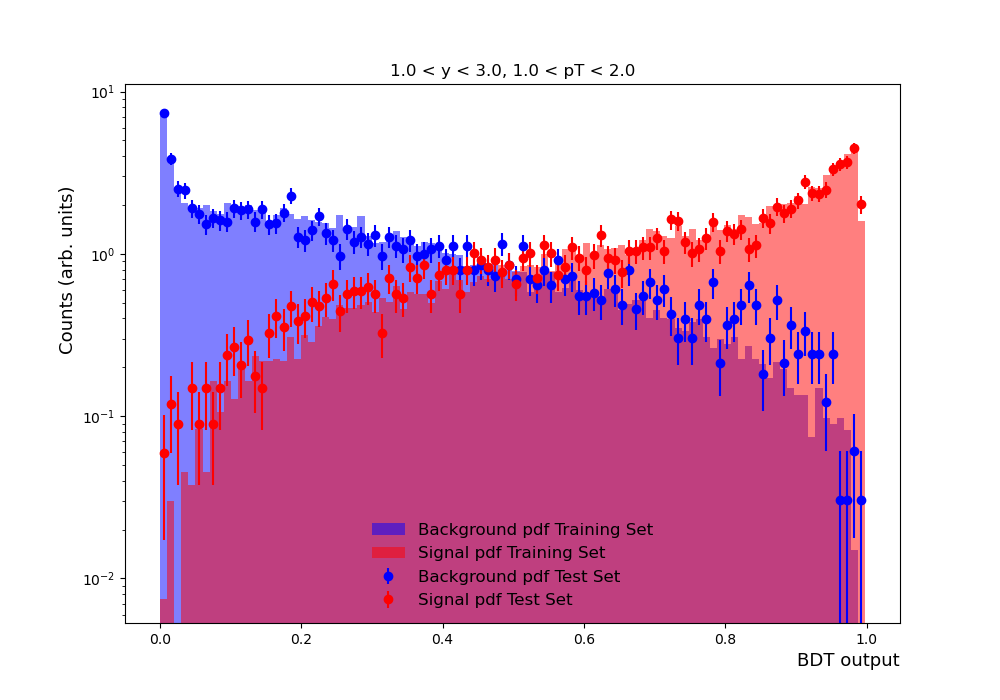
\includegraphics[width=0.45\linewidth]{gallery/results2/fav_train_test.png}
%     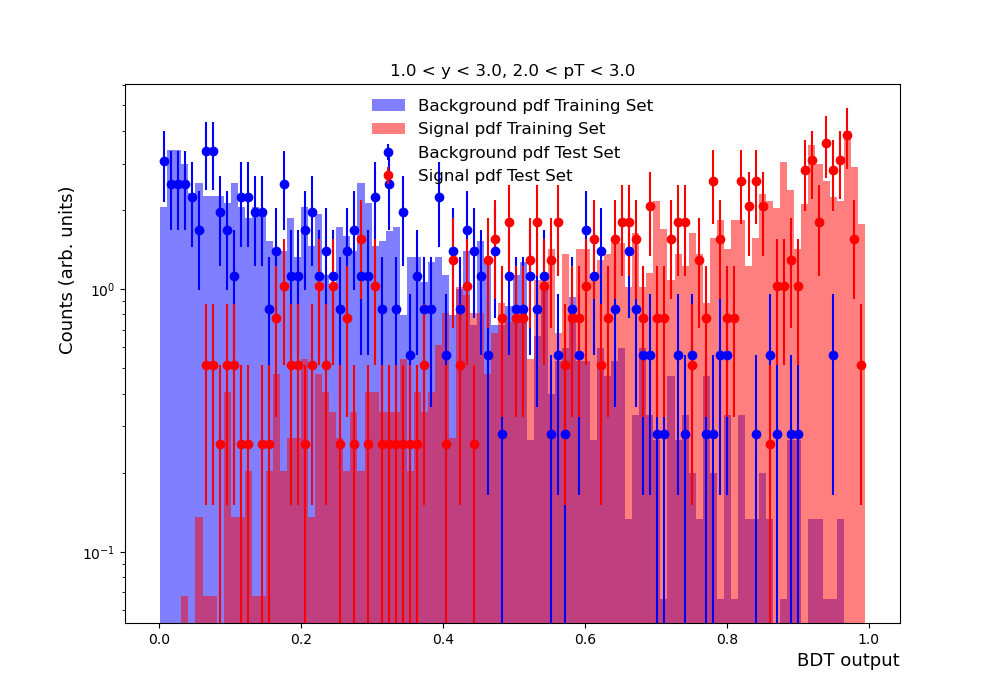
\includegraphics[width=0.45\linewidth]{gallery/results2/all_train_test.png}
%     \caption{BDT output distributions for training and testing data in $1<y<3$ and $2<p_T<3~{\rm GeV/c}$. The left plot shows results for a BDT trained using the selected 9 features, and the right plot shows results for a BDT trained using all 13 features.}
%     \label{f.bdt_all_vs_fav}
% \end{figure}
% %
% In Fig. \ref{f.bdt_all_vs_fav}, we observe that the BDT with 13 features (right plot) exhibits much flatter output distributions, which indicates a less clearly delineated separation between signal and background candidates. {\color{brown} What else to say about this? How to interpret and explain the worse performance???}

%
\begin{figure}[h!]
    \centering
    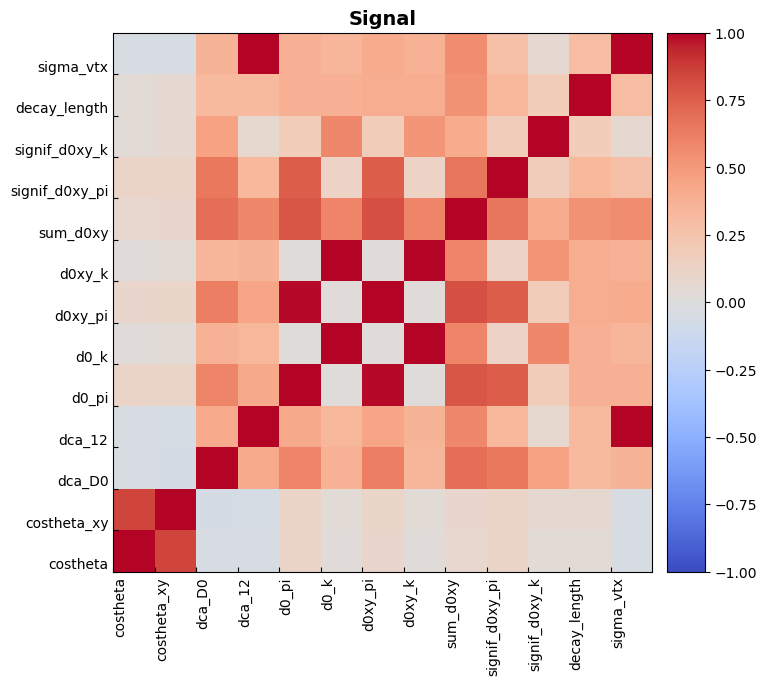
\includegraphics[width=0.8\linewidth]{gallery/results2/all_correlation_plot_sig.png}
    \caption{Correlation coefficients of all 13 topological features, for signal candidates in $1<y<3$ and $2<p_T<3~{\rm GeV/c}$. A value of 1 (dark red) indicates perfect positive correlation, and a value of -1 (dark blue) indicates perfect negative correlation.}
    \label{f.all_corr}
\end{figure}
%
Fig. \ref{f.all_corr} shows the correlations between these features. As expected, features defined with respect to one another---\texttt{costheta} and \texttt{costheta\_xy}, \texttt{dca\_12} and \texttt{sigma\_vtx}, as well as the various measurements for DCA of the pion and kaon---are positively correlated. However, our results demonstrate that BDTs are surprisingly robust to feature correlations. This makes sense given that BDTs tend to systematically favor the use of one feature over another when the two are highly correlated, and thus the models remain largely unaffected by the redundancies introduced by correlations. Nonetheless, it is generally advisable to eliminate strong correlations between features in order to improve the computational efficiency of the BDT and the interpretability of the results.

%---------------------------
\subsection{Tuning BDT hyperparameters}
\label{sec.results_hyperparams}

For the last aspect of our BDT optimization, we examine the impacts on model performance that can result from choices made during hyperparameter optimization. In our analysis, we utilize Optuna \cite{Optuna} to optimize the first five hyperparameters listed in Ch. \ref{sec.ml_optuna}. We consider \texttt{n\_estimators}, \texttt{max\_depth}, and \texttt{learning\_rate} to be the ``basic" hyperparameters, and we consider \texttt{min\_child\_weight} and \texttt{min\_split\_loss} to be less essential ``regulatory" hyperparameters.

In case I, we optimize the three basic hyperparameters, restricting them to the relatively conservative ranges:
\begin{itemize}
    \item \texttt{n\_estimators}: (100, 400)
    \item \texttt{max\_depth}: (1, 3)
    \item \texttt{learning\_rate}: (0.01, 0.1)
\end{itemize}
with all other hyperparameters set to default values. This is the same condition as in the preliminary analysis. In case II, we then expand the ranges to:
\begin{itemize}
    \item \texttt{n\_estimators}: (100, 800)
    \item \texttt{max\_depth}: (1, 8)
    \item \texttt{learning\_rate}: (0.01, 0.3)
\end{itemize}
Lastly in case III, we optimize the two regulatory hyperparameters alongside the initial three:
\begin{itemize}
    \item \texttt{n\_estimators}: (100, 800)
    \item \texttt{max\_depth}: (1, 8)
    \item \texttt{learning\_rate}: (0.01, 0.3)
    \item \texttt{min\_child\_weight}: (1, 10)
    \item \texttt{min\_split\_loss}: (0, 5)
\end{itemize}

In Table \ref{tab.optuna}, we list the best hyperparameter values determined by Optuna in each of the three cases for $1<y<3$ and $1<p_T<2~{\rm GeV/c}$. We notice that when given greater flexibility, Optuna tends to select large values for \texttt{max\_depth}. In case III, we also observe a larger value for \texttt{n\_estimators}, which reaches beyond the original range set in case I. Although in cases II and III, the values of other hyperparameters decrease to offset the increase in \texttt{max\_depth} (and \texttt{n\_estimators}), we find that these hyperparameter values result in overfitting. This can be observed in the ROC curves of Fig. \ref{f.bdt_hyperparams}, which compares the results for case I and case III.

\begin{table}[h!]
    \centering
    \begin{tabular}{l|c|c|c}
         &  Case I & Case II & Case III \\
         \hline
         \texttt{n\_estimators} & 480 & 347 & 728 \\
         \texttt{max\_depth} & 3 & 6 & 8 \\
         \texttt{learning\_rate} & 0.067 & 0.034 & 0.011 \\
         \texttt{min\_child\_weight} & 1 & 1 & 10 \\
         \texttt{min\_split\_loss} & 0 & 0 & 1
    \end{tabular}
    \caption{Best hyperparameter values selected by Optuna for the three cases examined in $1<y<3$ and $1<p_T<2~{\rm GeV/c}$. \texttt{min\_child\_weight} = 1 and \texttt{min\_split\_loss} = 0 are default values.}
    \label{tab.optuna}
\end{table}

%
\begin{figure}[h!]
    \centering
    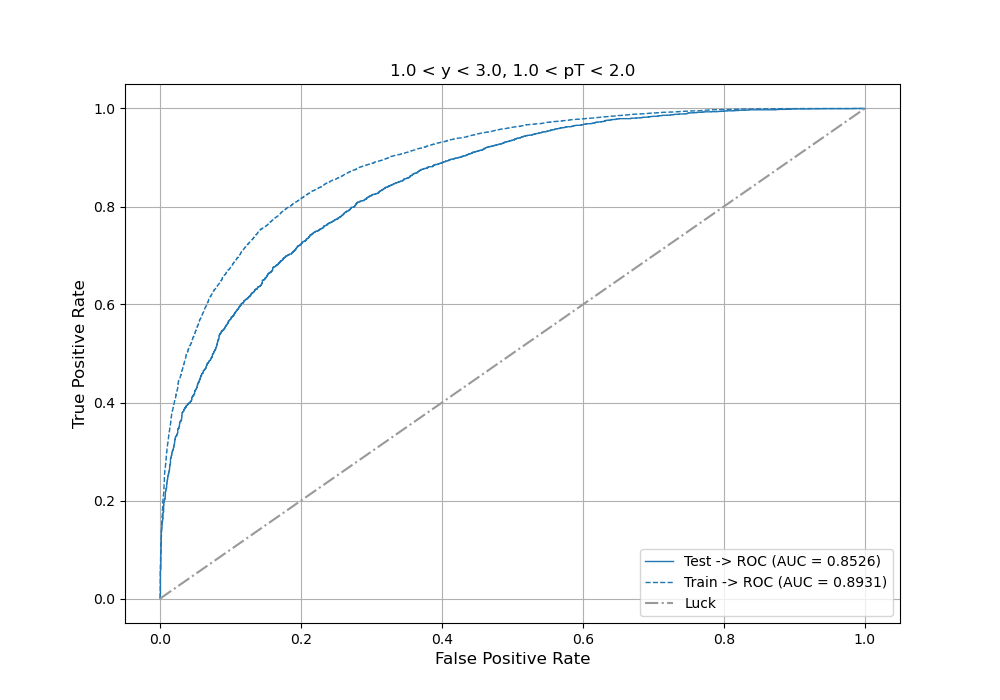
\includegraphics[width=0.5\linewidth]{gallery/results2/fav_roc_train_test.png}
    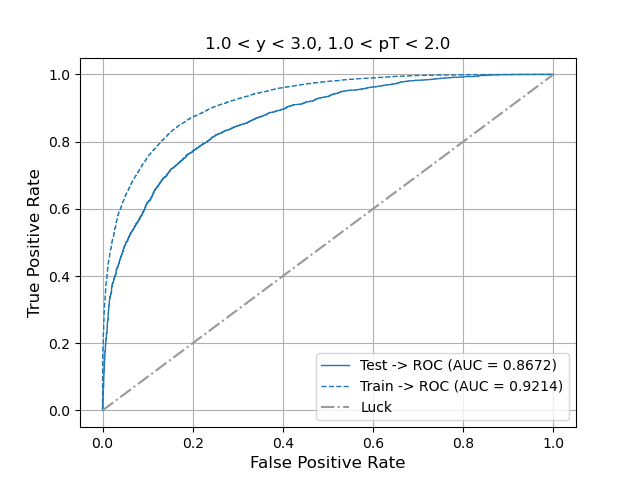
\includegraphics[width=0.46\linewidth]{gallery/results2/fav_roc_train_test_5params.png}
    \caption{ROC curves for training data (dashed line) and testing data (solid line) for BDTs with different hyperparameter optimization condition, in $1<y<3$ and $1<p_T<2~{\rm GeV/c}$. The left plot shows results for case I (Test AUC = 0.8526, Train AUC = 0.8931), and the right plot shows results for case III (Test AUC = 0.8672, Train AUC = 0.9214).}
    \label{f.bdt_hyperparams}
\end{figure}
%
In case III (right plot), we observe greater discrepancies in the ROC curves and AUC values between training and testing data. Even with increased regularization via \texttt{min\_child\_weight} and \texttt{min\_split\_loss}, the high values for the basic hyperparameters are enough to cause overfitting. We do also observe a higher AUC value for the testing data in case III (0.8672) than in case I (0.8526), which suggests that the model which overfits the training data does perform slightly better on testing data. 

It is likely the case that BDT performance does not drop significantly with increased overfitting \cite{BDT}, which may explain Optuna's tendency to find hyperparameter values that overfit. Based on these results, we favor the use of the more restrictive ranges for the basic hyperparameters, as in case I. Alternatively, stronger regularization may also work to prevent overfitting.

%
% \begin{figure}[h!]
%     \centering
%     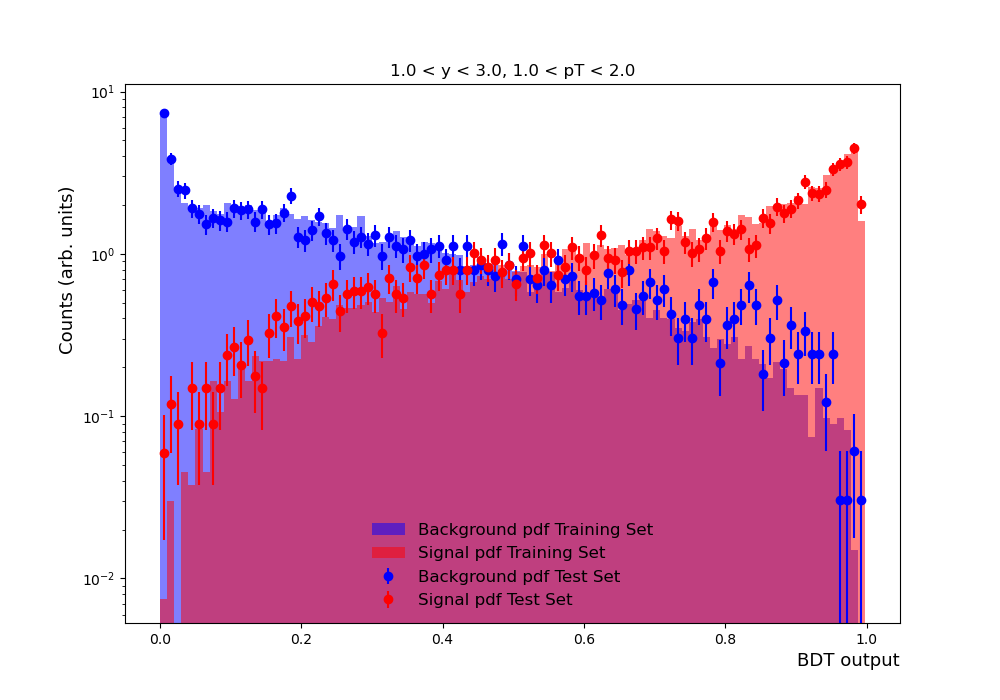
\includegraphics[width=0.5\linewidth]{gallery/results2/fav_train_test.png}
%     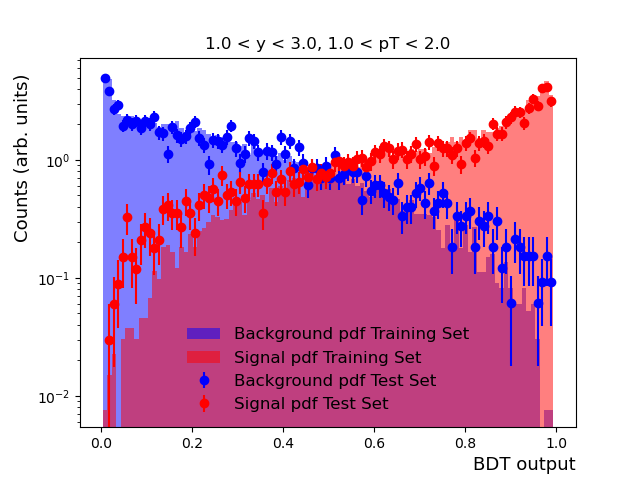
\includegraphics[width=0.46\linewidth]{gallery/results2/fav_train_test_5params.png}
%     \caption{BDT output distributions of training vs. test data for samples without (left) and \textbf{with (right)} machine-background effects. In both plots, training data are plotted as shaded histograms and test data are plotted as solid markers, with background candidates in blue and $D^0$ signal candidates in red.}
%     \label{f.roc_hyperparams}
% \end{figure}
%

%---------------------------------------------------------
\section{Comparison of BDT based method to non-ML analysis}
\label{sec.results_box_cuts}

Finally, we conclude our analysis with a comparison of BDT results to the box cuts on topological features, which we would normally apply for non-machine learning based studies. Focusing on $-1<y<1$ and $2<p_T<3~{\rm GeV/c}$ as an example, we obtain the box cuts from a previous $D^0$ analysis by the STAR Collaboration \cite{STAR}, which we list in Table \ref{tab.box_cuts}. We then train a BDT model using the six features for the same kinematic slice.

\begin{table}[h!]
    \centering
    \begin{tabular}{l|c}
         Feature & Cut \\
         \hline
         Decay Length (mm) & $>0.232$ \\
         ${\rm DCA_{12}}$ (mm) & $<0.063$ \\
         ${\rm DCA_{D0}}$ (mm) & $<0.040$ \\
         ${\rm DCA_{\pi}}$ (mm) & $>0.097$ \\
         ${\rm DCA_{K}}$ (mm) & $>0.094$ \\
         $\cos{\theta}$ & $>0.95$
    \end{tabular}
    \caption{Box cuts on $D^0\rightarrow\pi+K$ topology for $-1<y<1$ and $2<p_T<3~{\rm GeV/c}$, from the STAR Collaboration \cite{STAR}.}
    \label{tab.box_cuts}
\end{table}

%
\begin{figure}[h!]
    \centering
    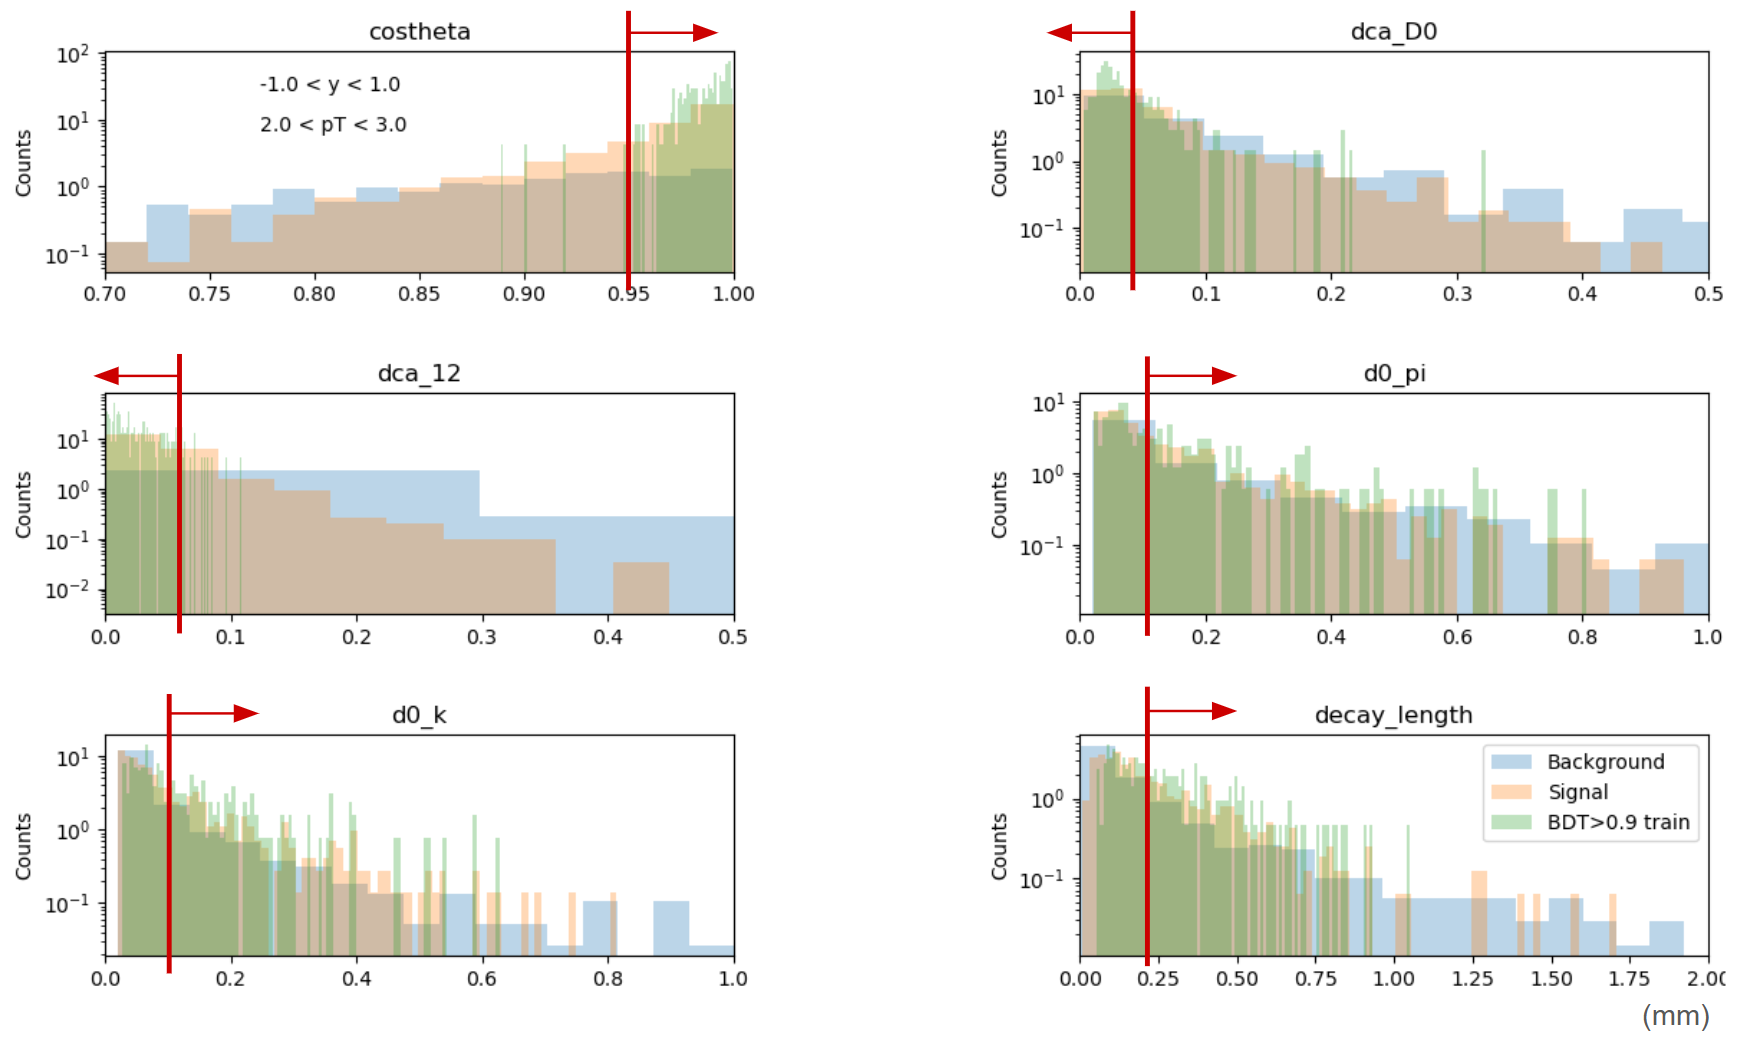
\includegraphics[width=0.9\linewidth]{gallery/results2/top_BDT_vs_box.png}
    \caption{Topological distributions of candidates in the training dataset for $-1<y<1$ and $2<p_T<3~{\rm GeV/c}$, comparing true signal candidates (orange), true background candidates (blue), candidates selected for BDT output $>0.9$ (green), and candidates selected by box cuts (red arrow) from the STAR Collaboration analysis \cite{STAR}.}
    \label{f.bdt_vs_box}
\end{figure}
%
In Fig. \ref{f.bdt_vs_box}, we plot the topological distributions of the true signal candidates (orange) and true background candidates (blue) in the training data, along with the candidates accepted by the BDT for a threshold of 0.9 (green) and those accepted by the box cuts in Table \ref{tab.box_cuts} (red arrows). We choose the BDT threshold value to yield the most similar S/B ratio as that obtained using the box cuts, and we obtain the selected candidates by applying the model onto its training data (without additional resampling). Comparing the BDT selections and box cuts, we observe that both generally favor candidates toward the same side of each distributions. For example, both tend to accept candidates with high values of $\cos{\theta}$, low values of ${\rm DCA_{D0}}$, low values of ${\rm DCA_{12}}$, etc. However, the BDT selections are much more flexible than the hard cutoffs of the box cuts. 

Interestingly, we observe that the BDT selections and box cuts are quite similar for $\cos{\theta}$ and ${\rm DCA_{12}}$, which are the two most important features according to the mean SHAP values. These selections also make sense intuitively, since we expect perfectly reconstructed $D^0$ signals to have $\cos{\theta}=1$ and ${\rm DCA_{12}}=0$. These observations offer some confidence that the BDT is learning the true signal-and-background boundaries, consistent with what we can expect from our physical intuition and from non-ML methods of analysis. 

%
\begin{figure}[h!]
    \centering
    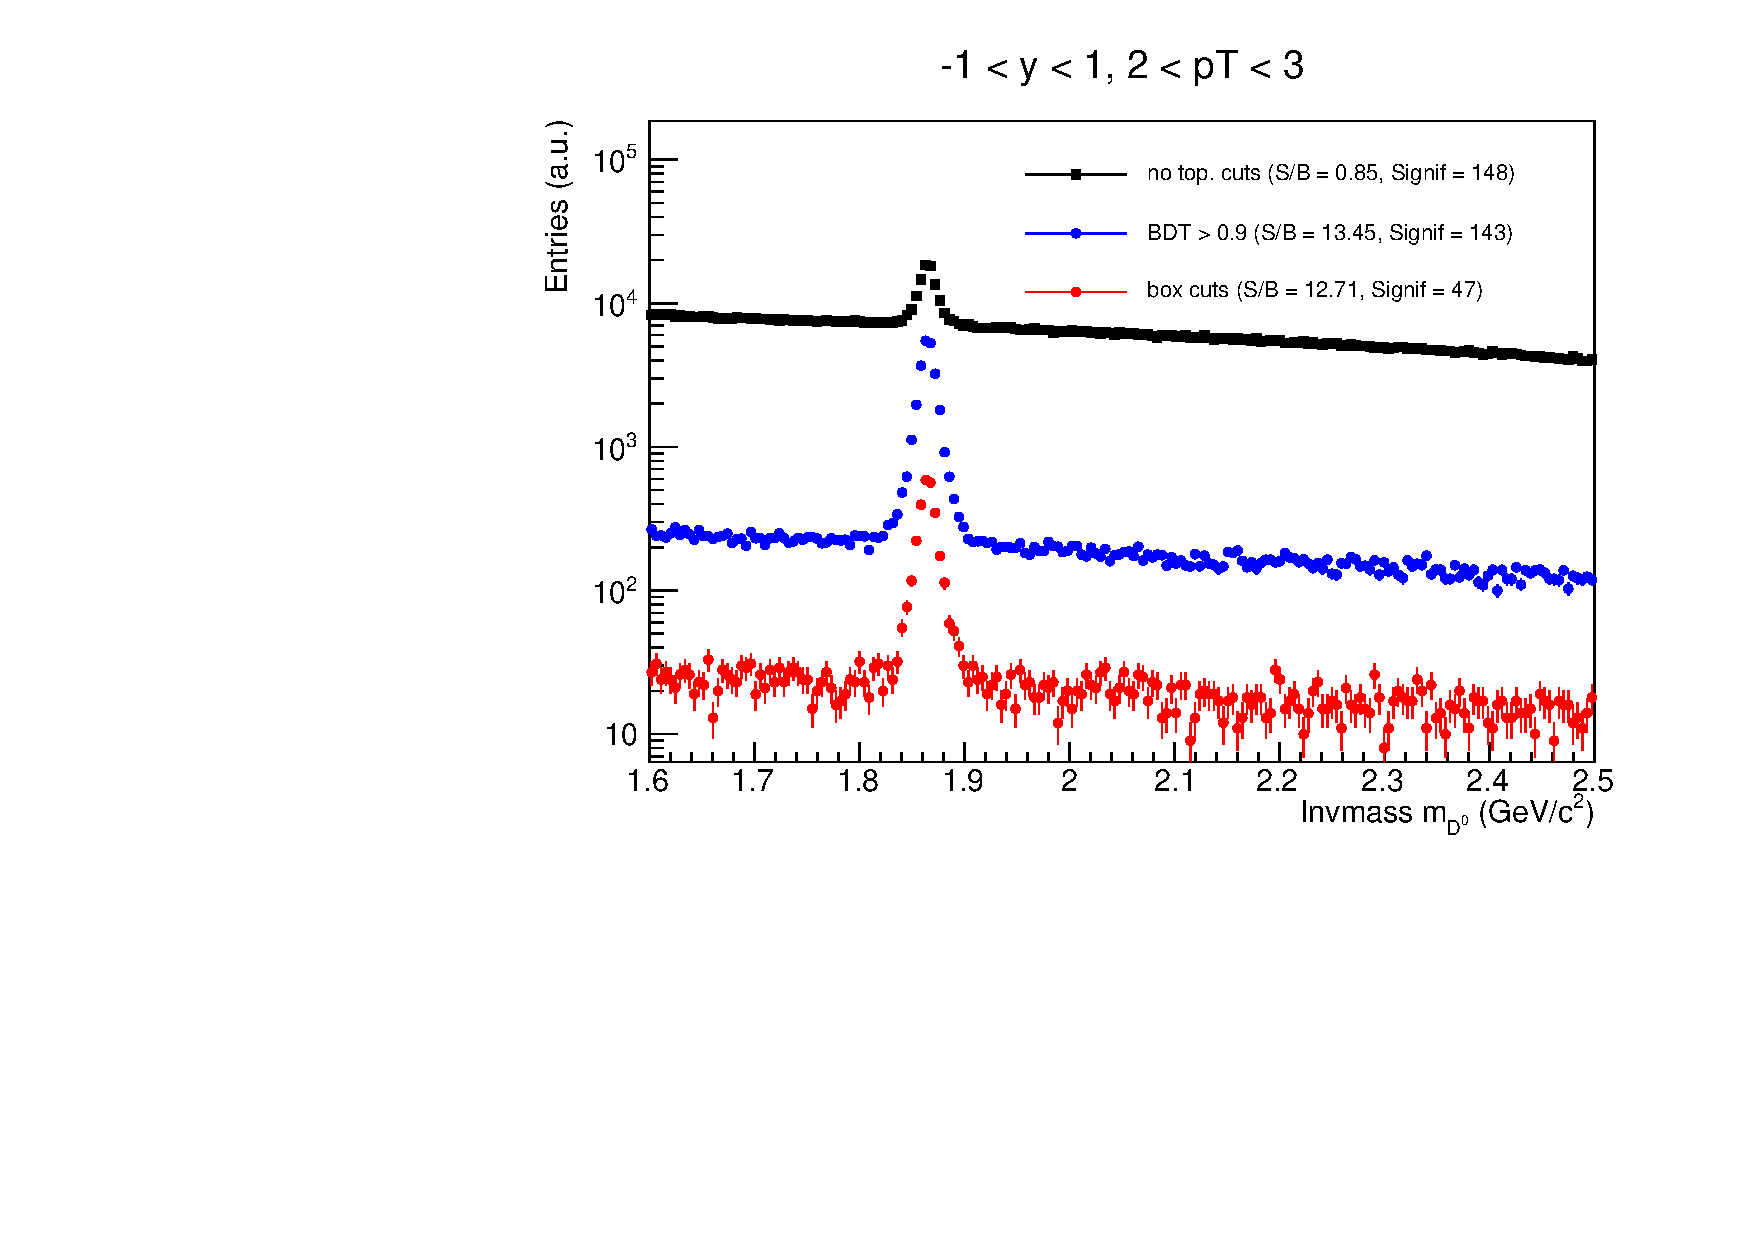
\includegraphics[width=0.65\linewidth]{gallery/results2/inv_mass_ML_vs_box_cuts_y_-1.0_1.0_pt_2.0_3.0_bdt_0.9.pdf}
    \caption{Reconstructed $D^0$ invariant mass distributions before BDT (black), after applying box cuts (red), and after applying BDTs selections (blue), for $2<p_T<3~{\rm GeV/c}$. The BDT threshold is selected to yield the S/B most similar to that of the box cuts.}
    \label{f.inv_mass_box}
\end{figure}
%
Comparing the $D^0$ invariant mass distributions in Fig. \ref{f.inv_mass_box}, we find that for similar S/B values, the BDT selections yield a much greater Significance than the box cuts. The ability of the BDT to preserve higher statistics and thus produce higher Significance illustrates an important advantage of the ML method over traditional box cuts.
\chapter{Summary and outlook}
\label{conclusion}

In summary, in this thesis we have explored the application of boosted decision trees to the separation of $D^0$ signals and background at the EIC. In Ch. \ref{ch:d0_top}, we examined the features of $D^0\rightarrow\pi+K$ decay topology which we utilize to distinguish true $D^0$ signals from background, and we noted the dependence of the topological distributions on $y$ and $p_T$ of the $D^0$. In Ch. \ref{ch.ml}, we introduced the BDT methodology which we applied to $D^0$ analysis in Ch. \ref{ch.results}. We first utilized an existing framework \cite{Shyam_ml} to analyze new simulated data samples in Ch. \ref{sec.results_bkg_study}, producing a preliminary analysis which demonstrated the negative impacts of machine-background effects on the effectiveness of $D^0$ invariant mass reconstruction. We then improve upon the BDT framework in Ch. \ref{sec.results_optimization}, separately analyzing the data in slices of $y$ and $p_T$, optimizing the BDT threshold to maximize the Significance, testing the various combinations of topological features, and adjusting the selection of BDT hyperparameters using Optuna. 

Through these analyses, we observed varying results in different Ch. \ref{sec.results_prelim} slices, with the forward $y$ and low $p_T$ region exhibiting the least effective signal-and-background separation but the greatest improvement in Significance after BDT application. In Ch. \ref{sec.results_features}, we found that changing the feature selection can improve the results in some kinematic slices, particularly ones with lower statistics, while producing negligible effect in others. We note that more features does not generally lead to better BDT performance. Then in Ch. \ref{sec.results_hyperparams}, we observed a tendency for Optuna to select hyperparameter values which lead to overfitting, suggesting the need to restrict the ranges of basic hyperparameters to more conservative values. Finally, in Ch. \ref{sec.results_box_cuts} we illustrated the greater flexibility and greater improvements provided by BDT based analysis compared to traditional box cuts on topological features.

In future work, the steps taken in Ch. \ref{sec.results_optimization} to optimize the BDT framework can be applied to improve the analysis of data samples with machine-background effects, which would provide a more realistic demonstration of $D^0$ invariant mass reconstruction for actual EIC experiments. Additionally, there remains multiple avenues to explore in the tuning of BDT hyperparameters with Optuna. Firstly, expanding the range of regulatory hyperparameters and/or optimization of additional hyperparemeters (listed in Ch. \ref{sec.ml_optuna}) may be able to effectively prevent overfitting. Secondly, Optuna provides different sampling and optimization algorithms \cite{Optuna_docs} which it uses to traverse the parameter space, which can also impact the resulting hyperparameter values selected. These aspects can be examined to better understand and control the tendency of overfitting for different kinematic slices.

% NOTE: If you have only one appendix, use the command \appendix instead
% of \appendices.
%
% \appendix
\appendices

% Be sure to set \appendix or \appendices in structural/body.tex
%\chapter{Some theoretical background}
%\label{app.theory}
%Unlike Classical particles, elementary particles obey the laws of quantum mechanics and special relativity. Combining both theories gives {\it quantum field theory}, which is the backbone of the Standard Model. In this appendix, we present a simplified overview of important concepts in quantum mechanics and special relativity. (This is appendix is by no means a comprehensive review, but may hopefully provide some context for background knowledge mentioned in the body of this thesis.) For undergraduates interested in learning more about the theories, below are a few textbook recommendations:
%\begin{itemize}
%    \item Quantum mechanics:
%    \begin{itemize}
%        \item {\it Introduction to Quantum Mechanics} by Griffiths \& Schroeter \cite{Griffiths_Schroeter}
%    \end{itemize}
%    \item Special relativity, quantum field theory, and particle physics: 
%    \begin{itemize}
%        \item {\it Introduction to Elementary Particles} by Griffiths \cite{Griffiths}
%        \item {\it A Standard Model Workbook} by Moore \cite{Moore}=
%        \item {\it Quarks \& Leptons: An Introductory Course in Modern Particle Physics} by Halzen \& Martin \cite{Halzen_Martin}
%    \end{itemize}
%\end{itemize}

%-------------------------
%\section{Quantum mechanics}
%\label{sec.quantum}

%At very small distance scales, systems are governed by quantum physics, exhibiting both particle-like and wave-like properties. In quantum mechanics, the state of a system is given by a {\it wavefunction} $\ket{\psi}$, which is a vector in a complex-valued vector space, called Hilbert space. $\ket{\psi}$ obeys all the properties of vectors. In particular, it can be written as a linear combination of vectors in any basis of our choice.

%Additionally, $\ket{\psi}$ evolves in time according the {\it Schrodinger equation}, which is a wave equation, and thus also obeys all the properties of waves. For example, wavefunctions propagate and interfere with each other. In the common position-basis, the {\it amplitude} of the wavefunction is given by $\psi(\mathbf{x},t)$, and the Schrodinger equation looks like
%\begin{equation}
%    i\frac{\partial}{\partial t}\psi(\mathbf{x},t) = -\frac{1}{2m}\nabla^2\psi(\mathbf{x},t) + V(\mathbf{x})\psi(\mathbf{x},t) \ ,
%\end{equation}
%where the spatial derivative term represents the kinetic energy, and the $V(\mathbf{x})$ term represents the potential energy.
% For a free particle, where $V(\mathbf{x})=0$, the wavefunction is a {\it plane wave},
% \begin{equation}
%     \psi(\mathbf{x},t)=Ae^{i(\mathbf{p}\cdot\mathbf{x}-Et)} \ ,
% \end{equation}
% where $\mathbf{p}$ is the momentum of the particle, $E$ is the total energy of the particle, and $A$ is a normalization constant chosen such that
% \begin{equation}
%     |\psi(\mathbf{x},t)|^2=1 \ .
% \end{equation}
% Thus, we interpret $\psi(\mathbf{x},t)$ as a {\it probability amplitude}.

%Another condition that wavefunctions must satisfy is {\it normality}, given by
%\begin{equation}
%    |\braket{\psi|\psi}|^2 \equiv 1 \ , 
%    \label{eqn.norm}
%\end{equation}
%or, in terms of the position basis amplitude,
%\begin{equation}
%    \int_{-\infty}^\infty d^3\mathbf{x} \ |\psi(\mathbf{x},t)|^2 \equiv \int_{-\infty}^\infty d^3\mathbf{x} \ \psi^*(\mathbf{x},t)\psi(\mathbf{x},t) \equiv 1 \ .
%    \label{eqn.norm2}
%\end{equation}
%Eq. \eqref{eqn.norm} and \ref{eqn.norm2} define the inner product of the wavefunction with itself, which is equal to its magnitude squared. (This is analogous to taking the inner product, or dot product, of the vector $\mathbf{x}=(x,y,z)$, which gives the length of the vector squared: $|\mathbf{x}|^2\equiv\mathbf{x}\cdot\mathbf{x}=x^2+y^2+z^2$. In Eq. \eqref{eqn.norm2}, $\psi(\mathbf{x},t)$ is a complex-valued function, so the inner product also includes an integral and complex conjugation.)

%Since the integral in Eq. \eqref{eqn.norm2} is equal to 1, we interpret $|\psi(\mathbf{x},t)|^2$ as a probability density, and $\psi(\mathbf{x},t)$ as a {\it probability amplitude}. More generally, the inner product of any two states $\ket{\psi_1}$ and $\ket{\psi_2}$, denoted $\braket{\psi_1|\psi_2}$ or $\braket{\psi_2|\psi_1}$, represents a probability. For example, in order to determine the probability of a system transitioning from some initial state $\ket{\psi_i}$ to some final state $\ket{\psi_f}$, we take the squared inner product $|\braket{\psi_f|\psi_i}|^2={\rm Prob}_{i\rightarrow f}$. In fact, in high energy experiments, many measurements boil down to determining the probability that some initial set of particles transitions into some final set of particles after they collide.

% {\color{brown} Due to the probabilistic nature of quantum mechanics, particles and systems do not have definite properties, such as position, momentum, energy, etc., until we ``observe" them, or measure them. When we perform a measurement, our interaction with the system {\it collapses} the wavefunction into a definite state..........

 % Heisenberg uncertainty principle? Observables?}
% \begin{itemize}
%     \item measurement and wavefunction collapse (system becomes particle-like)
% \end{itemize}

%---------------------------------------------------------
\chapter{Some concepts in special relativity}
\label{sec.relativity}
Unlike Classical particles, elementary particles obey the laws of quantum mechanics and special relativity. Combining both theories gives {\it quantum field theory}, which is the backbone of the Standard Model. In this appendix, we present a simplified overview of important concepts in special relativity, which may serve to provide context for some of the background knowledge mentioned in the body of this thesis.
%For undergraduates interested in learning more about the theories, below are a few textbook recommendations:
%\begin{itemize}
%    \item Special relativity, quantum field theory, and particle physics: 
%    \begin{itemize}
%        \item {\it Introduction to Elementary Particles} by Griffiths \cite{Griffiths}
%        \item {\it A Standard Model Workbook} by Moore \cite{Moore}=
%        \item {\it Quarks \& Leptons: An Introductory Course in Modern Particle Physics} by Halzen \& Martin \cite{Halzen_Martin}
%    \end{itemize}
%\end{itemize}

%-------------------------
\section{Four-vectors and Lorentz transformations}
When objects travel near the speed of light, as particles do in high energy experiments, they obey relativistic physics. In special relativity, space and time are treated on equal footing, as coordinates in {\it spacetime} (also known as Minkowski space). Position $\mathbf{x}$ and time $t$ are then combined into a new object, called a {\it four-vector},
\begin{equation}
    \tilde x \equiv \begin{pmatrix}
        t \\
        \mathbf{x}
    \end{pmatrix}\
    =\begin{pmatrix}
        t \\
        x \\
        y \\
        z
    \end{pmatrix}\ . \label{eqn.xmu}
\end{equation}
Like any other type of vector, four-vectors can be added, scaled, and transformed via linear transformations, or matrices. (Commonly, bold-faced symbols like $\mathbf{x}$ are used to denote ``regular" three-dimensional vectors while four-vectors are denoted with non-bold symbols like $x$. Here, we instead use $\tilde{x}$ to denote the position four-vector in order to avoid confusion with the coordinate $x$.) In standard notation, the components of a four-vector are denoted $\tilde x^\mu$, where the index $\mu=0,1,2,3$ acts as a label. For example, $\tilde{x}^0=t$ for $\mu=0$, $\tilde{x}^1=x$ for $\mu=1$, etc.

If we want to change from one reference frame to another, we must apply a rotation of the spacetime coordinates, known as a {\it Lorentz transformation}. In other words, we need to rotate the four-vector $\tilde{x}$. To implement transformations on a four-vector, we need $4\times 4$ matrices of the form
\begin{equation}
    M = \begin{pmatrix}
        M^0_0 & M^0_1 & M^0_2 & M^0_3 \\
        M^1_0 & M^1_1 & M^1_2 & M^1_3 \\
        M^2_0 & M^2_1 & M^2_2 & M^2_3 \\
        M^3_0 & M^3_1 & M^3_2 & M^3_3 \\
    \end{pmatrix} \ ,
\end{equation}
where $M^\mu_\nu$ is the element in row $\mu$ column $\nu$, with $0$ being the time index and $1,2,3$ being the $x,y,z$ indices. Regular spatial rotations, such as
\begin{equation}
    \Lambda_R = \begin{pmatrix}
        1 & 0 & 0 & 0 \\
        0 & \cos{\theta} & -\sin{\theta} & 0 \\
        0 & \sin{\theta} & \cos{\theta} & 0 \\
        0 & 0 & 0 & 1
    \end{pmatrix} \ ,
\end{equation}
which rotates a four-vector about the $z$-axis by some angle $\theta$, are a form of Lorentz transformation. (Remember the $0$-th row and column correspond to time.) 

Additionally, there is another type of Lorentz transformation, called a {\it boost}, which allows us to transform between two reference frames that are moving relative to each other. For example, consider a particle traveling at velocity $\beta$ in the $+x$ direction relative to a stationary observer. From the stationary observer's frame, we can boost into the moving particle's frame by multiplying all the coordinates by the Lorentz transformation matrix
\begin{align}
    \Lambda_B = \begin{pmatrix}
        \gamma & -\gamma\beta & 0 & 0 \\
        -\gamma\beta & \gamma & 0 & 0 \\
        0 & 0 & 1 & 0 \\
        0 & 0 & 0 & 1 
    \end{pmatrix} \ , \label{eqn.boost}
\end{align}
where $\gamma = 1/\sqrt{1-\beta^2}$. (Note that in natural units, the speed of light is $c=1$. Particles cannot travel faster than the speed of light, so $\beta \leq 1$, which means $\gamma \ge 1$.) 

%-------------------------
\section{The relativity of time and distance}
Suppose we, as the stationary observer, measure the time and distance traveled by a particle (which is moving with velocity $\beta$) to be $\Delta\tilde x=(\Delta t, \Delta x, \Delta y, \Delta z)$. If we boost to the particle's frame, we will see that the particle measures its own travel time and distance to be $\Delta\tilde x'=(\Delta t', \Delta x', \Delta y', \Delta z')$, where
\begin{equation}
    \begin{pmatrix}
        \Delta t' \\
        \Delta x' \\
        \Delta y' \\
        \Delta z'
    \end{pmatrix}
    = \begin{pmatrix}
        \gamma & -\gamma\beta & 0 & 0 \\
        -\gamma\beta & \gamma & 0 & 0 \\
        0 & 0 & 1 & 0 \\
        0 & 0 & 0 & 1 
    \end{pmatrix}
    \begin{pmatrix}
        \Delta t \\
        \Delta x \\
        \Delta y \\
        \Delta z
    \end{pmatrix} \\
    = \begin{pmatrix}
        \gamma(\Delta t-\beta\Delta x) \\
        \gamma(-\beta \Delta t + \Delta x) \\
        \Delta y \\
        \Delta z
    \end{pmatrix} \ .
    \label{eqn.lorentz}
\end{equation}
In general, Eq. \eqref{eqn.lorentz} shows that measurements made by two observers do not agree if they are traveling with relative motion between them. Thus, distances and time intervals are no longer absolute, but are relative.

Two important consequences of relativity are {\it time dilation} and {\it length contraction}. Roughly speaking, time dilation describes the phenomenon in which a moving observer will experience time passing more slowly relative to a stationary observer. Length contraction describes the phenomenon in which the length of a moving object will be shortened along its direction of motion. In high energy collisions, this means that unstable particles traveling near the speed of light live longer than their average lifetimes (as measured for the particles at rest), and they become ``pancaked" along their direction of travel. The larger the $\gamma$ (or velocity $\beta$), the stronger the effects.

%-------------------------
\section{Lorentz-invariance}
Although distances and time are now relative, there is still a way to define absolute lengths. In normal three-dimensional space, we measure lengths by taking the dot product of the position vector $\mathbf{x}$ with itself, $|\mathbf{x}|^2 = \mathbf{x}\cdot\mathbf{x} = x^2+y^2+z^2$. In spacetime, distances are given by the inner product of a four-vector with itself, which is defined
\begin{equation}
\begin{aligned}
    \tilde{x}^2 &= \tilde{x}\cdot\tilde{x} \equiv t^2 - \mathbf{x}^2 \\
    &= t^2-x^2-y^2-z^2 \ . 
\end{aligned}
\end{equation}
Note that there is a relative sign difference between the time component and spatial components. The reason we define the inner product this way is because this quantity is actually {\it Lorentz-invariant}, meaning that its value is the same in every reference frame. 

More generally, the inner product of any four-vector object with itself is Lorentz-invariant. One important example is the momentum four-vector,
\begin{equation}
    p \equiv \begin{pmatrix}
        E \\
        \mathbf{p}
    \end{pmatrix}
    = \begin{pmatrix}
        E \\
        p_x \\
        p_y \\
        p_z
    \end{pmatrix}
    = \begin{pmatrix}
        \gamma m \\
        \gamma m v_x \\
        \gamma m v_y \\
        \gamma m v_z
    \end{pmatrix}\ , \label{eqn.four_momentum}
\end{equation}
where $E$ is energy, and $\mathbf{p}$ is the three-dimensional momentum vector, $m$ is mass, and $\mathbf{v}=(v_x,v_y,v_z)$ is the three-dimensional velocity vector. The $\gamma$ factor accounts for the relativistic motion. For particles traveling with small momenta, $\gamma\approx 1$, and $p\approx(m, mv_x,mv_y,mv_z)$.
\begin{equation}
\begin{aligned}
    p^2 = p \cdot p &= E^2-|\mathbf{p|^2} \\
    &=  \gamma^2m^2(1-|\mathbf{v}|^2) = \frac{1}{1-\beta^2}m^2(1-\beta^2) \\
    &= m^2,
    \label{eqn.mass}
\end{aligned}
\end{equation}
Putting back the factors of $c$, Eq. \eqref{eqn.mass} reads $E^2-(|\mathbf{p}|c)^2 = (mc^2)^2$. In the rest frame of a particle (in which $\mathbf{p}=0$), this reduces to Einstein's famous equation $E=mc^2$. 

Lorentz-invariance is essential, as it ensures that the laws of physics are the same in every reference frame. Thus, when describing high-energy particle traveling near the speed of light, we must take care that all our equations are built from Lorentz-invariant quantities.

%-------------------------
\section{Rapidity}
In analogy to spatial rotations, we can also write a Lorentz boost as a hyperbolic rotation between space and time. For example, a boost along the $x$-direction is given by
\begin{align}
    \Lambda_B = \begin{pmatrix}
        \cosh{y} & -\sinh{y} & 0 & 0 \\
        -\sinh{y} & \cosh{y} & 0 & 0 \\
        0 & 0 & 1 & 0 \\
        0 & 0 & 0 & 1
    \end{pmatrix} \ , \label{eqn.boost2}
\end{align}
where
\begin{equation}
    y\equiv \tanh^{-1}(\beta) \label{eqn.y}
\end{equation}
is called the {\it rapidity}. (Eq. \eqref{eqn.boost2} represents the exact same transformation as Eq. \eqref{eqn.boost}.) Just like $\theta$ determines the amount by which a spatial rotation is performed, the rapidity $y$ determines how much a four-vector is boosted. The greater the relative velocity $\beta$ between two reference frames, the larger the $y$, and the greater the boost must be to go from one to the other. 

The more common expression for rapidity in particle physics is
\begin{equation}
    y = \frac{1}{2}\ln \left[ \frac{E+p_z}{E-p_z} \right] \ , \label{eqn.y2}
\end{equation}
written in terms of the energy $E$ and momentum $p_z$ of a particle. (We can always define the $z$-direction to be the particle's direction of motion relative to us.) We can see that Eq. \eqref{eqn.y} and \eqref{eqn.y2} are equivalent:
\begin{equation}
\begin{aligned}
    y &= \tanh^{-1}(\beta) \\
    &= \frac{1}{2}\ln \left[ \frac{1+\beta}{1-\beta} \right] \\
    &= \frac{1}{2}\ln \left[ \frac{\gamma m(1+\beta)}{\gamma m(1-\beta)} \right] \\
    &=\frac{1}{2}\ln \left[ \frac{E+p_z}{E-p_z} \right] \ ,
\end{aligned}
\end{equation}
where in the second line we have used the definition $\tanh^{-1}x = \ln [(1+x)/(1-x)]$, and in the last line we have used the definition of $E$ and $\mathbf{p}$ in Eq. \eqref{eqn.four_momentum} for a particle traveling in the $z$-direction.

One useful property of $y$ is that it is Lorentz-invariant, since it is specifically defined for two particular reference frames, whose relative velocity is always $\beta$. (Absolute velocities are not Lorentz-invariant, but relative velocities are.) Additionally, since $y$ is equal to the natural log of some quantity, as written in Eq. \eqref{eqn.y2}, rapidities obey simple addition and subtraction, and we do not need to deal with complicated Lorentz transformations like we would in order to add regular velocities.  Thus, we can think of rapidity as a ``relativistic version" of velocity that is easier to work with in particle physics.

%----------------------------------------------------------
% \chapter{Point-like scattering: the elastic $e\mu$ cross section}
% \label{app.emu}

% This interaction is mediated by a virtual photon, whose four-momentum $q\equiv(\nu, \mathbf{q})=k-k'$ is equal to the amount of four-momentum transferred between the electron and proton. A quick calculation reveals that
% \begin{equation}
%     q^2 = (k-k')^2 = 2k\cdot k' = 2EE'(1-\cos{\theta}) \ ,
% \end{equation}
% which is in general nonzero. Thus, $q^2\neq m_\gamma^2$, seemingly breaking the laws of relativity. Vaguely speaking, the Heisenberg uncertainty principle $\Delta E \Delta t \geq 1 / 2$ provides some leeway, allowing such particles to fluctuate into existence for an extremely brief, unobservable, amount of time. These particles are termed {\it virtual}, or {\it off-shell}.

%----------------------------------------------------------
\chapter{Data samples}
\label{app.samples}

Here we reference the PYTHIA-8 simulation samples used to complete this thesis, which are provided by the ePIC Collaboration \cite{ePIC}. We obtain signal candidates from ``D0" samples, which refer to $D^0$-enriched data in which every event in the sample contains at least one $D^0$ particle. We obtain background candidates from ``DIS" samples, which refer to minimum-bias data without $D^0$-enrichment.

For the examination of topological distributions in Ch. \ref{ch:d0_top}, we utilize the December 2024 campaign $ep$ simulations.
\begin{enumerate}
    \item D0 samples with $Q^2>1~{\rm GeV^2}$: \\
    /volatile/eic/EPIC/RECO/24.12.0/epic\_craterlake/SIDIS/D0\_ABCONV\\/pythia8.306-1.1/10x100/q2\_1/hiDiv/
    
    \item D0 samples with $Q^2>100~{\rm GeV^2}$: \\
    volatile/eic/EPIC/RECO/24.12.0/epic\_craterlake/SIDIS/D0\_ABCONV\\/pythia8.306-1.1/10x100/q2\_1/hiDiv/
    
\end{enumerate}

For machine learning analyses in Ch. \ref{ch.results}, we utilize the October 2025 campaign $ep$ simulations with $Q^2>1~{\rm GeV^2}$.
\begin{enumerate}
    \item Samples without machine-background effects
    \begin{enumerate}
        \item D0 samples: \\
        /volatile/eic/EPIC/RECO/25.10.3/epic\_craterlake/SIDIS/D0\_ABCONV\\/pythia8.306-1.1/10x100/q2\_1/hiDiv/
        
        \item DIS samples: \\
        /volatile/eic/EPIC/RECO/25.10.0/epic\_craterlake/DIS/NC/10x100\\/minQ2=1/

    \end{enumerate}
    \item Samples \textbf{with} machine-background effects
    \begin{enumerate}
        \item D0 samples: \\
        /volatile/eic/EPIC/RECO/25.10.4/epic\_craterlake\\/Bkg\_Exactly1SignalPer2usFrame/SIDIS/D0\_ABCONV\\/pythia8.306-1.1/10x100/q2\_1/hiDiv/
        
        \item DIS samples: \\
        /volatile/eic/EPIC/RECO/25.10.4/epic\_craterlake\\/Bkg\_1SignalPer2usFrame/DIS/NC/10x100/minQ2=1/

    \end{enumerate}
\end{enumerate}

The codes to obtain signal and background candidates are found in the directory \texttt{ML\_by\_slices/analysis\_jobs/} of the GitHub repository for this thesis \cite{github}, which is based on the analysis frameworks provided by Shyam Kumar \cite{Shyam_analysis} and Rongrong Ma \cite{Rongrong_jobs}.

%----------------------------------------------------------
\chapter{Data preparation for BDT and $D^0$ invariant mass plots}
\label{app.data_prep}

In this appendix, we describe the procedures to prepare the data for training BDT and plotting invariant mass distributions, after obtaining the signal and background candidates. The codes to implement the procedures are found in the Jupyter notebook \texttt{ML\_by\_slices/ML\_example\_results/ML\_by\_slices.ipynb} in our GitHub repository \cite{github} and is adapted from the machine learning framework provided by Shyam Kumar \cite{Shyam_ml}.

Here, we list the general steps and expand upon them in the following sections.
\begin{enumerate}
    \item Apply broad preselections, and select $y$ and $p_T$ ranges
    \item Fit $D^0$ invariant mass distributions of signal and background candidates
    \item Plot $D^0$ invariant mass distribution before BDT
    \begin{enumerate}
        \item Calculate the numbers of signal and background candidates expected for the desired number of events
        \item Randomly sample signal and background candidates from the fits
    \end{enumerate}
    \item Select signal and background datasets for BDT training
    \item Plot $D^0$ invariant mass distribution after BDT
    \begin{enumerate}
        \item Calculate the expected numbers of signal and background candidates selected by BDT
        \item Randomly sample signal and background candidates from the fits
    \end{enumerate}
\end{enumerate}


%------------------------
\section{Preselection and kinematic cuts}
\label{app.presel}
To reduce the size of the data we need to deal with, we first apply the following preselections on both signal and background candidates:
\begin{itemize}
    \item $1.6 < m_{D^0} < 2.5 ~{\rm GeV/c^2}$
    \item $0.02 < {\rm DCA_\pi}_{(xy)} < 10 ~{\rm mm}$
    \item $0.02 < {\rm DCA_K}_{(xy)} < 10 ~{\rm mm}$
    \item ${\rm Decay~Length} < 100 ~ {\rm mm}$
\end{itemize}
These broad cuts remove (mostly background) candidates far away from the expected $D^0$ invariant mass peak (around $1.86~{\rm GeV/c^2}$).

We then apply cuts on the $y$ and $p_T$ of the candidates to select the kinematic slice of interest.

%------------------------
\section{Training and testing data selections for BDT}
\label{app.presel}
We train the models on the ``raw" data obtained after preselection and kinematic cuts (not on the resampled data.) For training, we want the numbers of signal and background candidates to be the same. Thus, we resize the signal and background datasets (using randomized selection) to equal the minimum number of the two.

We also make additional invariant mass cuts on the signal and background candidates such that the signal candidates sit in or near the expected $D^0$ peak region and the background candidates sit in the sideband regions:
\begin{itemize}
    \item Signal cut: $1.7 < m_{D^0}<2.1$
    \item Background cut: $1.6 < m_{D^0}<1.7$ or $2.1 < m_{D^0}<2.5$
\end{itemize}

%------------------------
\section{Fits and resampling}
\label{app.resamp}

To produce the $D^0$ invariant mass plots, we scale up the number of signal and background candidates so that they correspond to the statistics expected in real EIC experiments. We do this by fitting the $D^0$ invariant mass distributions of the signal and background candidates, then randomly sampling the required numbers of candidates from those fitted distributions. Fig. \ref{f.resamp} illustrates examples of the data along with the fits and resampled distributions.

%
\begin{figure}[h!]
    \centering
    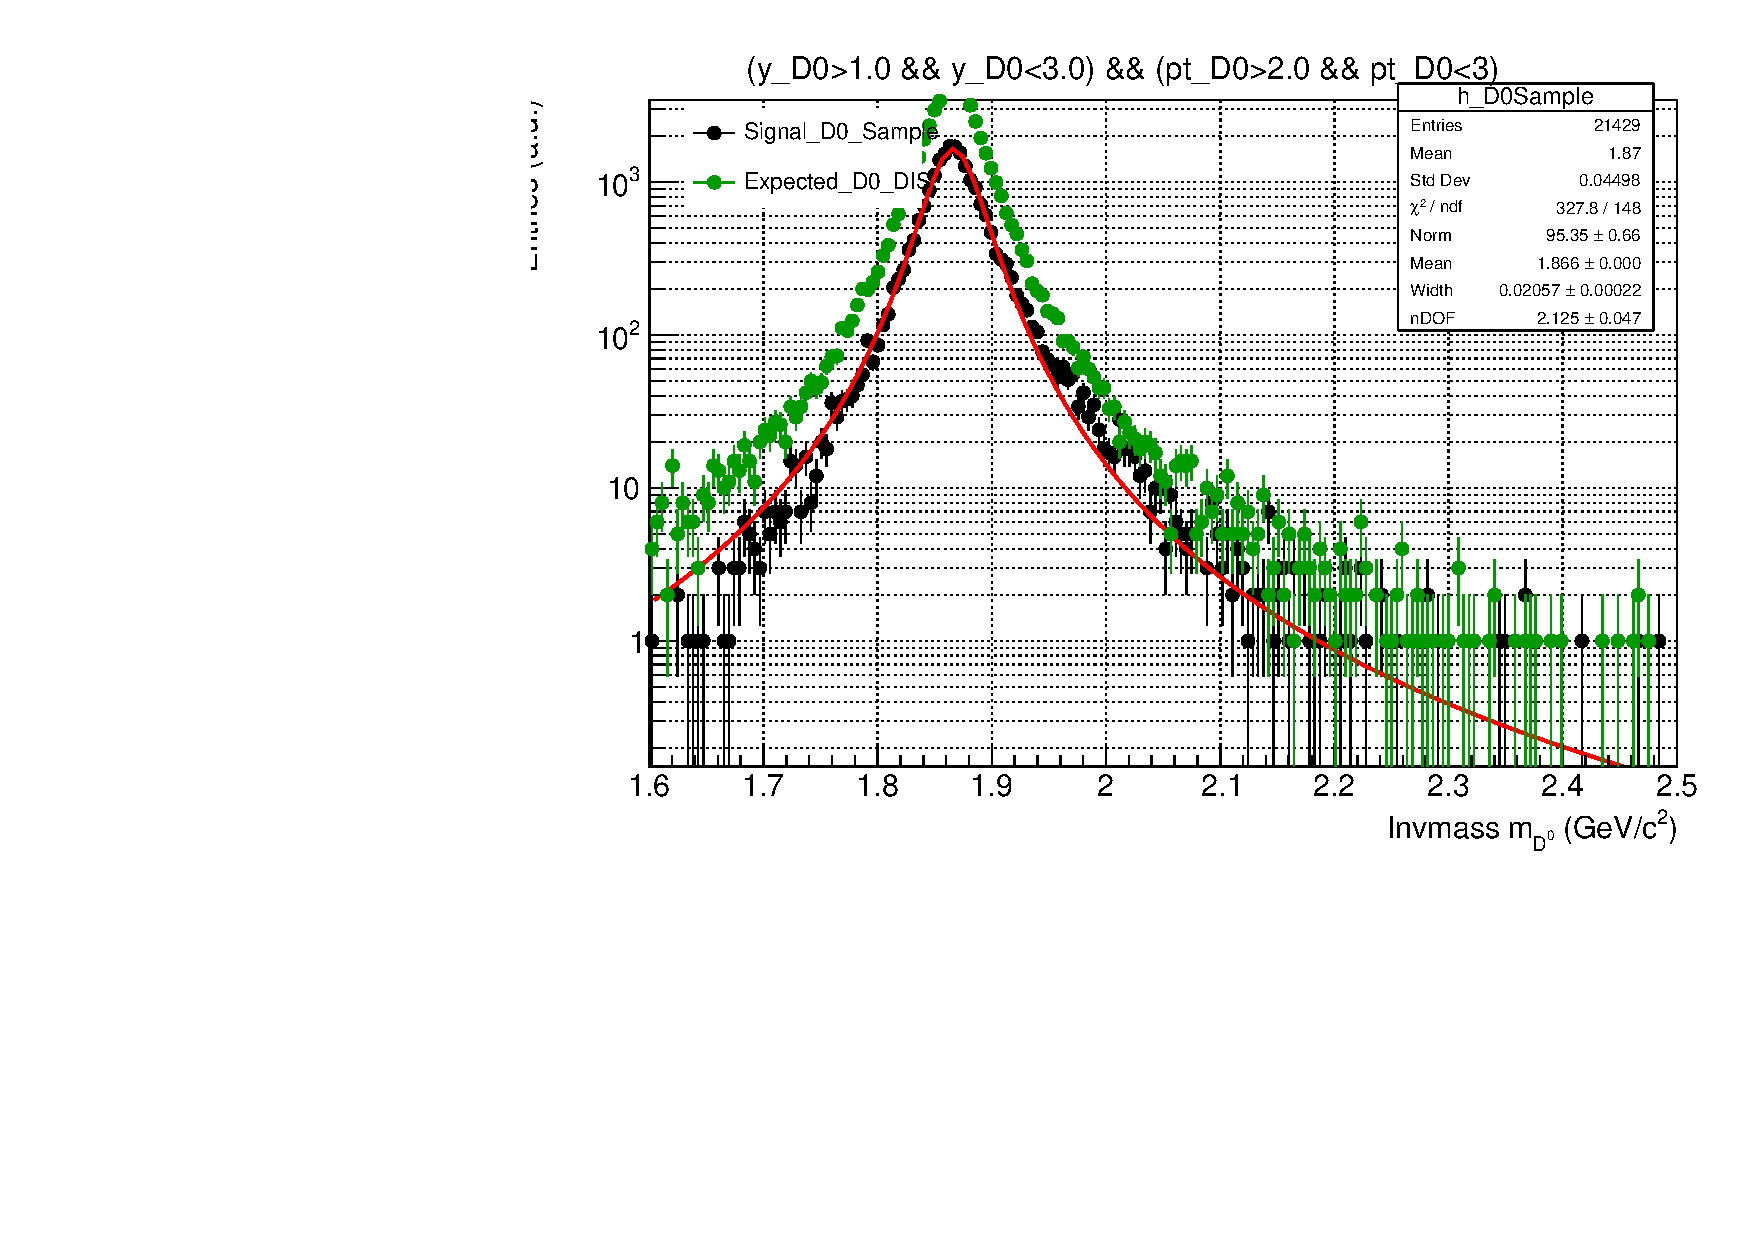
\includegraphics[width=0.6\linewidth]{gallery/appendix/resampled_signal_y_1.0_3.0_pt_2.0_3.0_before_ml.pdf}
    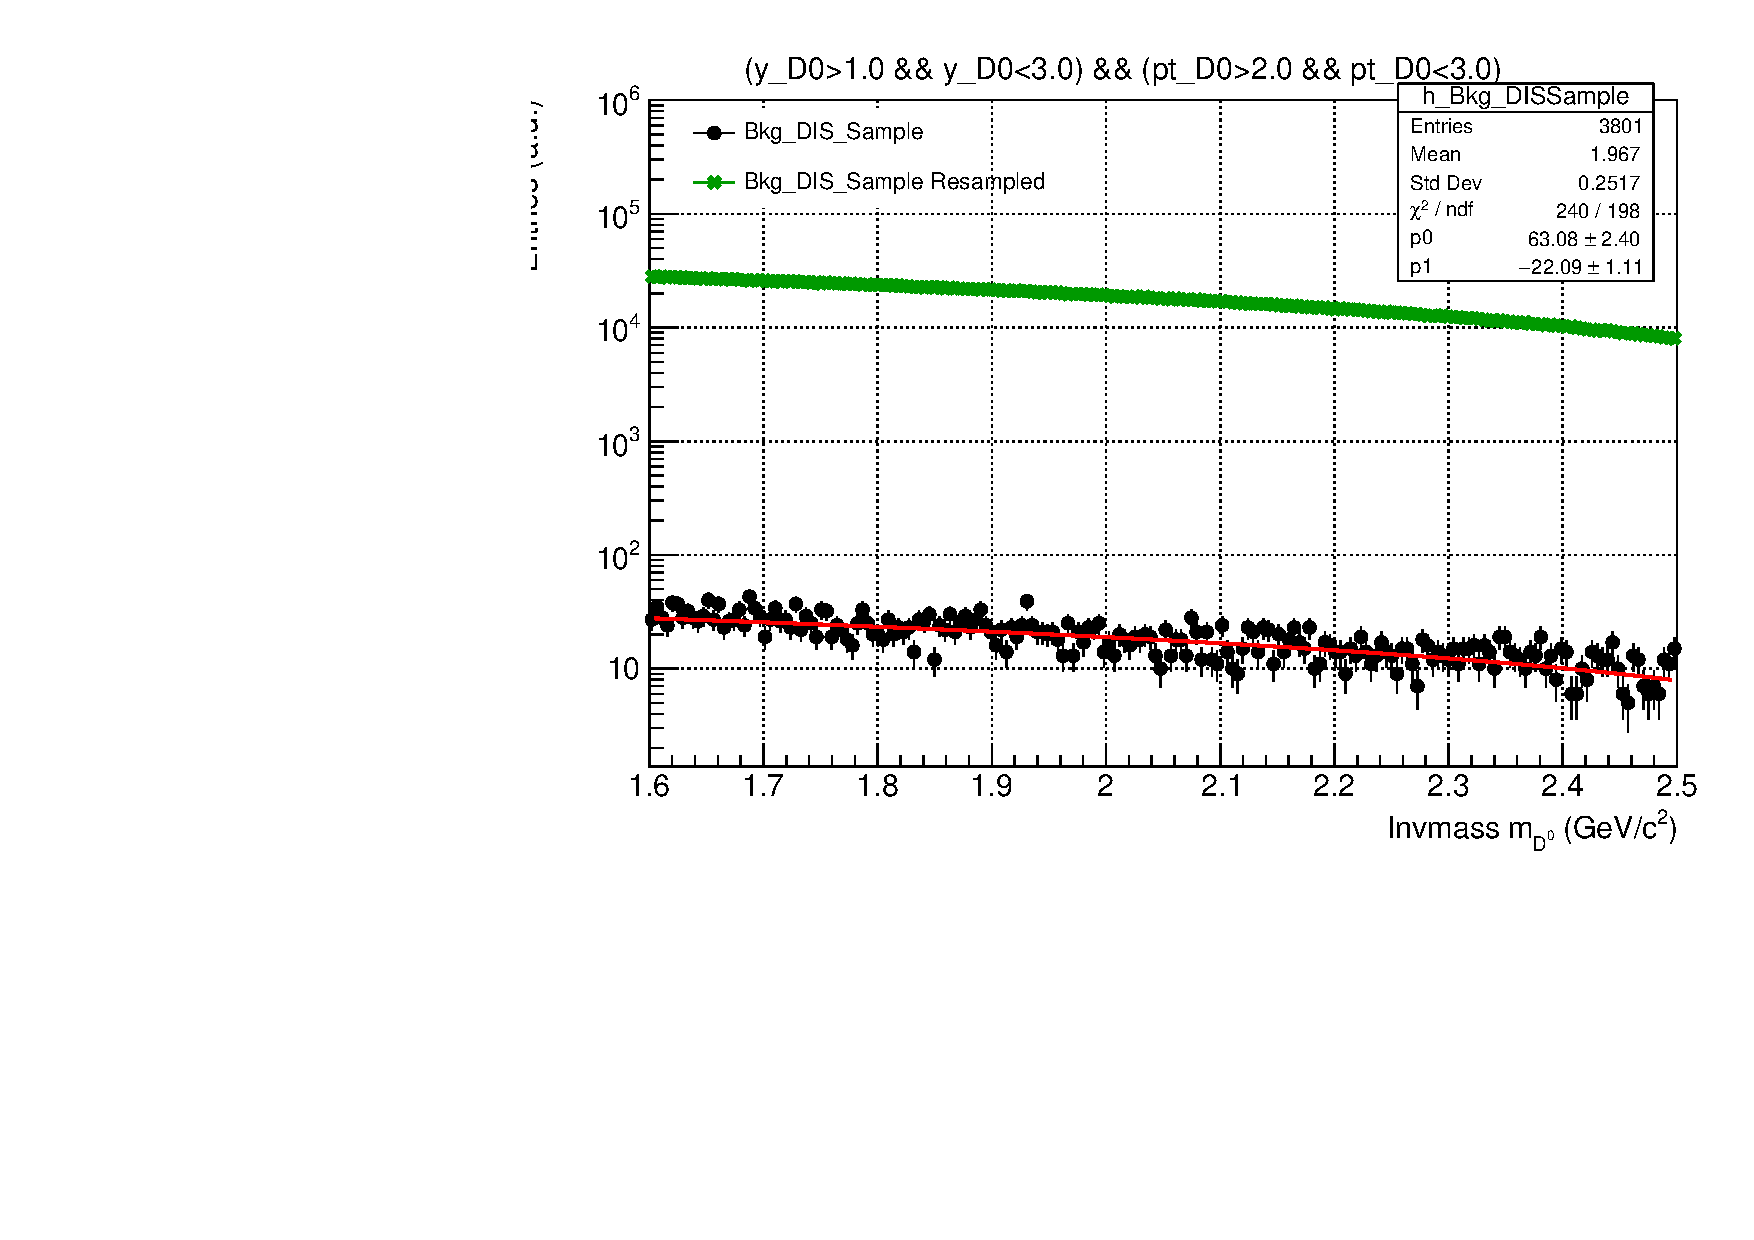
\includegraphics[width=0.6\linewidth]{gallery/appendix/resampled_bkg_y_1.0_3.0_pt_2.0_3.0_before_ml.pdf}
    \caption{Example fits to $D^0$ invariant mass distributions of signal (top) and background (bottom) candidates. Black markers indicate the original data, red curves indicate the fitted functions, and green markers indicate the resampled data. Signal distributions are fit using Student's $t$-distribution $f(x)=N\frac{\Gamma((\nu+1)/2)}{\sqrt{\nu\pi}\sigma\Gamma(\nu/2)}\left(1+\frac{(x-\mu)^2}{\sigma^2}\right)^{-(\nu+1)/2}$ with 4 free parameters: norm $N$, mean $\mu$, width $\sigma$, and nDOF $\nu$. Background distributions are fit using a second-degree polynomial $f(x)=p_0+p_1x+p_2x^2$ with 3 free parameters: $p_0$, $p_1$, and $p_2$.}
    \label{f.resamp}
\end{figure}
%
We fit the original $D^0$ invariant mass distribution (black) of the signal candidates with Student's $t$-distribution,
\begin{equation}
    f(x)={\color{purple} N}\frac{\Gamma(\frac{{\color{purple}\nu}+1}{2})}{\sqrt{{\color{purple}\nu}\pi} \ {\color{purple}\sigma} \ \Gamma(\frac{{\color{purple}\nu}}{2})}\left(1+\frac{(x-{\color{purple}\mu})^2}{{\color{purple}\sigma}^2}\right)^{-({\color{purple}\nu}+1)/2} \ ,
\end{equation}
where the norm $N$, mean $\mu$, width $\sigma$, and degrees of freedom (nDOF) $\nu$ are free parameters fitted to the data by a $\chi^2$ minimization procedure. This is a generalization of a Gaussian distribution with mean $\mu$ and standard deviation $\sigma$. We fit the distribution of background candidates with a second-degree polynomial,
\begin{equation}
    f(x)={\color{purple}p_0}+{\color{purple}p_1}x+{\color{purple}p_2}x^2 \ ,
\end{equation}
with free parameters $p_0$, $p_1$, and $p_2$. The best fit curves are shown in red in Fig. \ref{f.resamp}.

In our analyses, we work with the expected luminosity of $10 ~{\rm fb^{-1}}$, which corresponds to $4.72162\times10^9$ total events in each set of simulation samples. The number of expected background candidates is thus
\begin{equation}
    \hat{N}_{\rm bkg} = \frac{N_{\rm bkg}}{E_{\rm bkg}} \ \hat{E} \ , \label{eqn.Nbkg}
\end{equation}
where $\hat{N}_{\rm bkg}$ is the expected number of background candidates, $N_{\rm bkg}$ is the original number of candidates obtained from the DIS simulation samples, $E_{\rm bkg}$ is the number of events contained in those DIS samples, and $\hat{E} = 4.72162\times10^9$ is the expected total number of events.

The number of expected signal candidates is
\begin{equation}
    \hat{N}_{\rm sig} = \frac{N_{\rm sig}}{E_{\rm sig} S} \ \hat{E} \ , \label{eqn.Nsig}
\end{equation}
where an additional factor $S=1821.83$ is included to scale the number of events in the D0 samples to match that in the DIS samples.

To plot the $D^0$ invariant mass distribution before BDT, we randomly sample $\hat{N}_{\rm bkg}$ candidates from the fitted polynomial distribution and $\hat{N}_{\rm sig}$ candidates from the fitted Student's $t$-distribution, and plot all the candidates together. The resampled distributions are shown in green in Fig. \ref{f.resamp} and combine to form the black distribution for the data before BDT in Fig. \ref{f.inv_mass_ex}. We then calculate the S/B and Significance, 
\begin{align}
    {\rm S/B} &= \frac{\hat{N}_{\rm sig}^{D^0}}{\hat{N}_{\rm bkg}^{D^0}} \\
    {\rm Signif} &= \frac{\hat{N}_{\rm sig}^{D^0}}{\sqrt{\hat{N}_{\rm sig}^{D^0}+\hat{N}_{\rm bkg}^{D^0}}} \ ,
\end{align}
where $\hat{N}_{\rm sig}^{D^0}$ and $\hat{N}_{\rm bkg}^{D^0}$ are obtained by counting the number of resampled candidates within $2\sigma$ on each side of $\mu$ (with $\sigma$ and $\mu$ given by the fitted signal distribution).

%
\begin{figure}[h!]
    \centering
    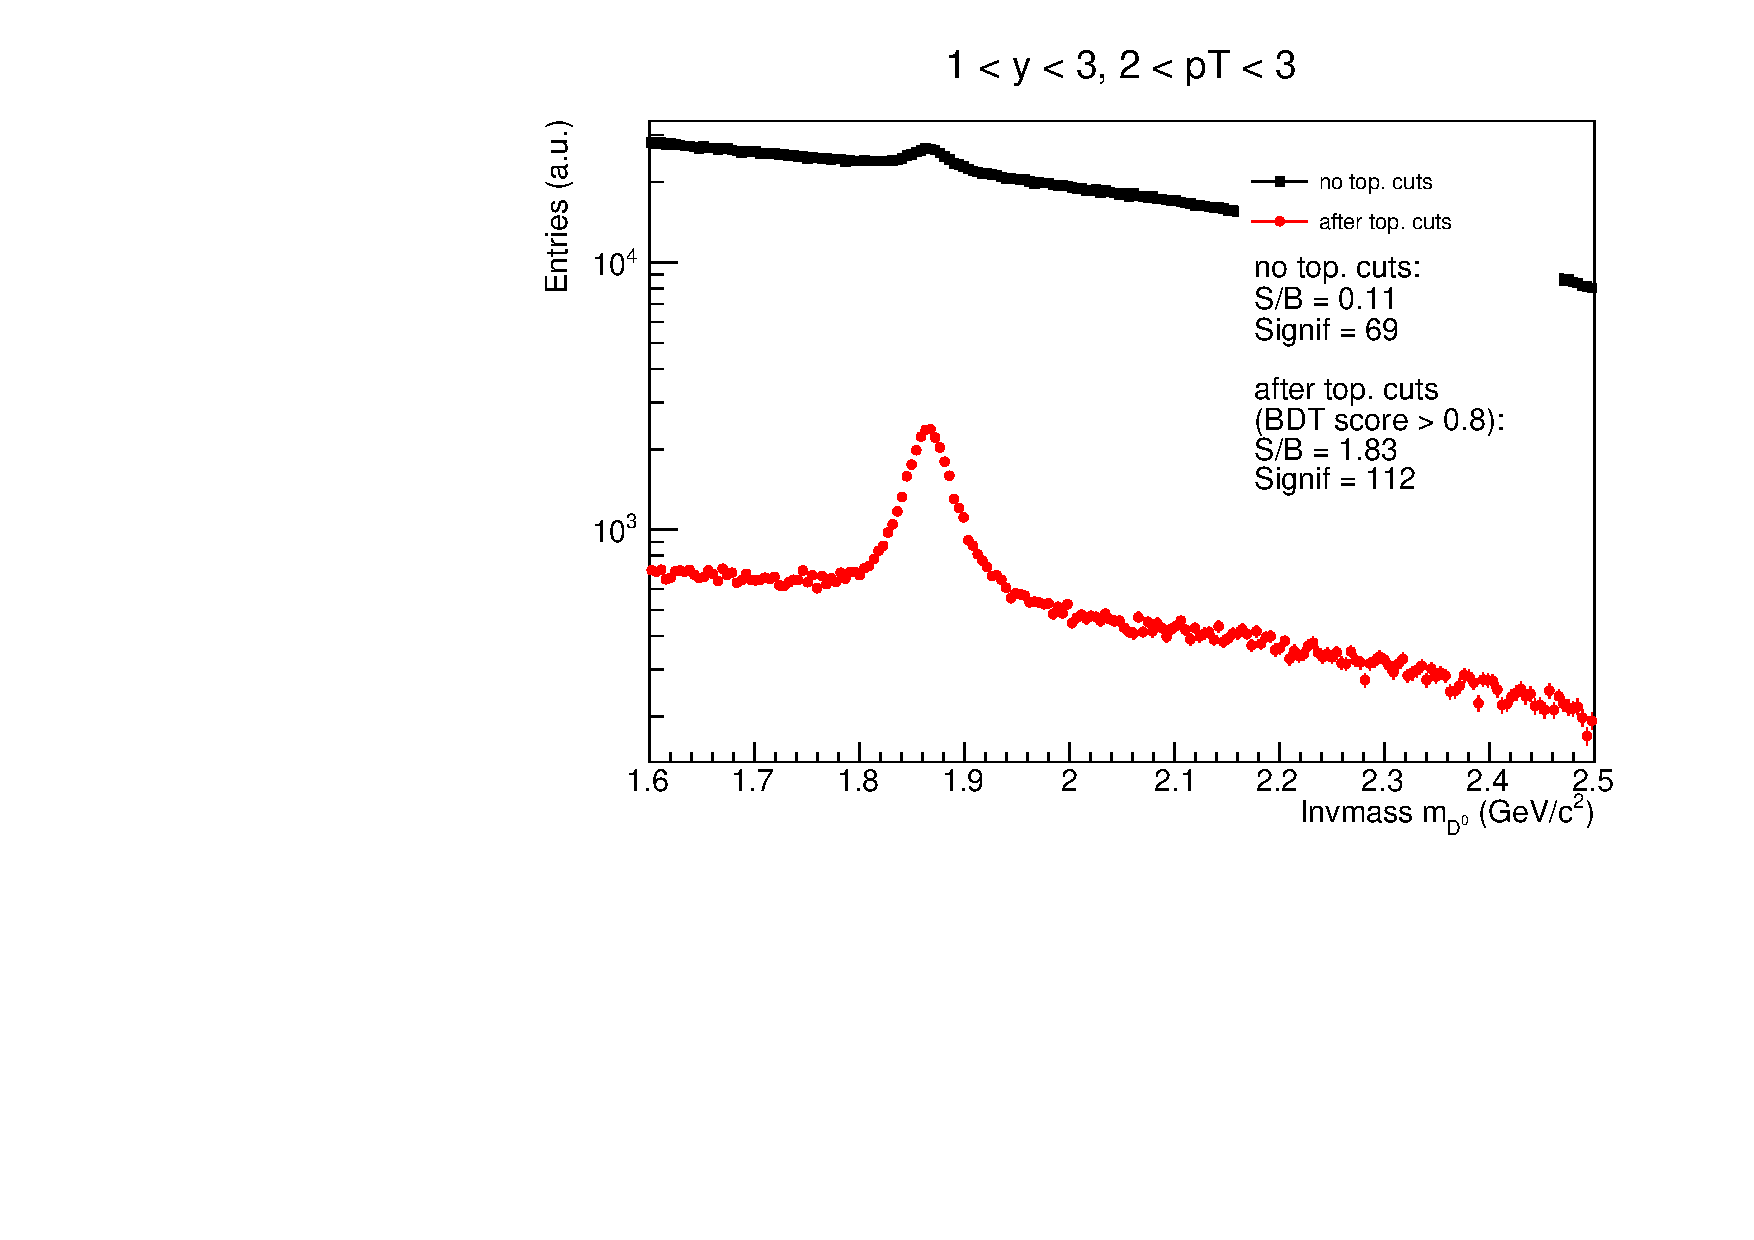
\includegraphics[width=0.7\linewidth]{gallery/appendix/inv_mass_before_and_after_ML_y_1.0_3.0_pt_2.0_3.0_bdt_0.8.pdf}
    \caption{Example $D^0$ invariant mass distributions of resampled candidates before BDT (black) and after BDT (red).}
    \label{f.inv_mass_ex}
\end{figure}
%

After performing the machine learning, we choose a BDT threshold $\hat{y}^*$ and obtain the corresponding efficiencies, $\epsilon_{\rm sig}(\hat{y}^*)$ and $\epsilon_{\rm bkg}(\hat{y}^*)$, which represent the fractions of signal and background candidates selected by the BDT. (The efficiencies are calculated using the raw data, but we generalize the results to the resampled data.) The numbers of resampled candidates after BDT are
\begin{align}
    \hat{N}^{BDT}_{\rm bkg} &= \hat{N}_{\rm bkg} \ \epsilon_{\rm bkg}(\hat{y}^*) \\
    \hat{N}^{BDT}_{\rm sig} &= \hat{N}_{\rm sig} \ \epsilon_{\rm sig}(\hat{y}^*)  \ ,
\end{align}
where $\hat{N}_{\rm bkg}$ and $\hat{N}_{\rm sig}$ are the numbers from Eq. \eqref{eqn.Nbkg} and \eqref{eqn.Nsig}.

To produce the red distribution for the data after BDT in Fig. \ref{f.inv_mass_ex}, we randomly sample $\hat{N}^{BDT}_{\rm sig}$ and $\hat{N}^{BDT}_{\rm bkg}$ candidates from the fitted signal and background distributions (the same ones from which we sampled the data before BDT). Finally, we calculate the S/B and Significance in the same manner as for the data before BDT.


%%%%%%%%%%%%%%%%%%%%%
% Optional glossary. May also be moved between the Table of Contents and the Text.
%%%%%%%%%%%%%%%%%%%%%
% \begin{glossary}
% \begin{description}
%     \item[\theauthor] A hard-working graduate student, nearing the end of this chapter of your education!
%     \item[\thedegree] \theauthor\ is about to earn this. Congratulations!
% \end{description}
% \end{glossary}

%%%%%%%%%%%%%%%%%%%%%%%%%%%%%%%%%%%%%%%%%%%%%%%%%%%%%%%%%%%%%%%%%%%%%%
% Generate the bibliography.					     %
%%%%%%%%%%%%%%%%%%%%%%%%%%%%%%%%%%%%%%%%%%%%%%%%%%%%%%%%%%%%%%%%%%%%%%
% \nocite{*}    % This command causes all items in the 		     %
                % bibliographic database to be added to 	     %
                % the bibliography, even if they are not 	     %
                % explicitly cited in the text. 		     %
\bibliographystyle{unsrtnat}  % Here the bibliography 		     %
\bibliography{references}        % is inserted.			     %
%%%%%%%%%%%%%%%%%%%%%%%%%%%%%%%%%%%%%%%%%%%%%%%%%%%%%%%%%%%%%%%%%%%%%%



%%%%%%%%%%%%%%%%%%%%%%%%%%%%%%%%%%%%%%%%%%%%%%%%%%%%%%%%%%%%%%%%%%%%%%
% Vita page.							     %
%%%%%%%%%%%%%%%%%%%%%%%%%%%%%%%%%%%%%%%%%%%%%%%%%%%%%%%%%%%%%%%%%%%%%%

% \begin{vita}

% \theauthor\ is going to graduate soon!
% \end{vita}
